\FloatBarrier

\section{Abstract}\label{abstract}

Which observations drive variance concentration in Transformer representations, and what can be read from the remaining variation? We examine point distributions within texts and evaluate shared principal components fixed on training articles. In both short texts and an article collection, the prominent long axis and its association with hidden-state norm at GPT-2's middle layer depended strongly on the first token. After that token was excluded from the analysis, a shared PCA basis retained position correlations on separate articles. Confirmatory tests also found positive median increments in current-token surprisal readout beyond a token-ID baseline, including comparisons among occurrences of the same token ID within an article. With a within-group training objective, four of six model--extraction-point conditions met the prespecified criteria, while two were inconclusive. Exploratory analyses located additional surprisal associations in PC2--8 and in vector direction after accounting for position and vector norm. They also showed that PC-versus-random rankings changed with training configuration and that positive median gains could coexist with severe losses on individual articles. Together, these results separate the observations responsible for conspicuous variance concentration from the variation supporting transferable readout, and show why both typical gains and article-level failures matter when interpreting principal components.

\textbf{Keywords:} Transformer, principal component analysis, norm, variance concentration, probing, within-token-ID variation, preregistration

\FloatBarrier

\clearpage
\section{1. Background and central claim}\label{background-and-central-claim}

A language model's hidden state is a vector representing a token after it has been processed. Projecting these vectors into a low-dimensional PCA space can reveal an elongated configuration and variation around it. When much of the variance lies along that long axis, which observations produce the concentration, and what can be read from the other components? Connecting a distant point to a dense cloud in token order can itself create a long line. Examining the observed point distribution is therefore the starting point for interpreting the shape.

Our central claim is that \textbf{the prominent variance concentration at GPT-2's middle layer depends strongly on the first token, while shared PCs fitted after excluding that token retain incremental current-token surprisal readout on separate articles beyond the specified lexical controls}. The latter result concerns median improvements across articles, including comparisons within article × token-ID groups containing repeated occurrences. We examine first-token sensitivity through point distributions and within-text measurements, and transferable readout through a basis and predictor fixed on training articles. A separate evaluation tests transfer of position correlations. Throughout, we distinguish coordinates fitted locally within a text from PCs shared across articles.

The study makes three contributions.

\begin{enumerate}
\def\labelenumi{\arabic{enumi}.}
\tightlist
\item
  \textbf{We identify the observations that drive concentration.} Point distributions in short texts and sensitivity measurements across articles show that the treatment of the first token strongly affects PC1 variance concentration and its association with the norm at GPT-2's middle layer. We also describe feature associations in local residuals and condition-dependent curve fits after final normalization.
\item
  \textbf{We establish incremental surprisal readout within recurring token IDs on separate articles.} Shared PCs improve on a fixed token-ID baseline and on random directions of the same dimensionality in the prespecified GPT-2 middle-layer comparison. The subsequent multi-model test evaluates a within-group training objective and reports both supported and inconclusive conditions.
\item
  \textbf{We characterize the sensitivity of readout evaluation.} Exploratory diagnostics identify component groups that support additional readout, examine the roles of vector length and direction, and reveal both changes in ranking across training configurations and the coexistence of typical improvements with large losses on a few articles.
\end{enumerate}

The study provides empirical diagnostics for assessing what can be concluded from visualizations and probes of hidden representations. We first present short-text geometry (Section 3), then confirmatory evaluations on separate articles (Section 4), followed by secondary comparisons and exploratory diagnostics (Sections 5 and 6). Section 7 discusses the implications, and Section 8 brings together the limitations and unresolved questions. Appendices A--C contain the main methods, supplementary summaries, inputs, and verification scope. Comprehensive tables and saved data are organized in the accompanying \href{../references/README.md}{reference materials}.

\FloatBarrier

\subsection{1.1 Relation to prior work}\label{relation-to-prior-work}

Ethayarajh {[}1{]} systematically examined anisotropy in contextualized representations. Luo et al.~{[}2{]} studied the relationship between outlier neurons and positional information in BERT and RoBERTa, while Sun et al.~{[}3{]} analyzed massive activations and their functions in LLMs. These findings motivate our examination of how a small number of coordinates or observations can strongly influence the global geometry of representation space.

For hidden-state visualization, Ning et al.~{[}4{]} considered high norms at the first position in GPT-2 and LLaMa, normalization to unit length, and the application of a fitted PCA transform to other states. Version 1 of that study describes an uncentered method that preserves the origin. We use centered PCA and separately measure occupancy, gaps between points, the contribution of the first token, and improvement from a linear to a quadratic fit. These measurements quantify which configurations of observations are summarized by concentrated variance.

We use linear probes {[}5{]} for feature readout and draw on control designs that account for a probe's capacity to memorize {[}6{]}. We extend these comparisons by fixing a token-ID baseline, shared coordinates, and readout coefficients on training articles, then evaluating surprisal increments on separate articles and within recurring article × ID groups. Random directions matched in dimensionality provide a further comparator. We also carry a training configuration identified through exploration into a subsequent evaluation on new articles, reporting median gains alongside individual failures.

The empirical contribution is to show that \textbf{strong first-token sensitivity of variance concentration can coexist with transferable surprisal readout beyond lexical mean differences}. The experiments further show that the PC-versus-random comparison depends on readout training configuration, and that positive median gains can conceal severe article-level losses. These findings connect geometric visualization to controlled readout evaluation while keeping local coordinates and shared PCs distinct.

\FloatBarrier

\section{2. Study design and measurements}\label{study-design-and-measurements}

\FloatBarrier

\subsection{2.1 Progression of the questions and levels of evidence}\label{progression-of-the-questions-and-levels-of-evidence}

The article experiments moved from sensitivity of concentration to transfer of feature associations and then to surprisal increments beyond lexical controls. Two exploratory steps informed later confirmations: the token-ID control was selected using P2 data and fixed for P3; within-group training was examined using the known P3 evaluation data and fixed for new training and evaluation articles in P4. We later explored article point distributions and added the short-text study. The presentation follows a conceptual path from geometry to readout, with Table 1 preserving the order and role of each stage.

For confirmatory experiments P1--P4, we fixed the targets, primary quantities, exclusions, comparisons, and decision rules in local protocol cards before collecting observations. EDA-0001--0004 are exploratory analyses of saved data informed by known results. For the short-text geometry study, P5, we explicitly treated the three inputs as known at design time and fixed the extraction points, measurements, and decision rules before new forward passes. We report P5 as geometric validation on known inputs and the primary hypotheses of P1--P4 as article-level confirmatory evaluations. Table 1 lists the roles and samples of each stage; Appendix A maps the full conditions to their fixed specifications.

\Needspace{6\baselineskip}\begingroup
\fontsize{9.3}{12}\selectfont\setlength{\tabcolsep}{3.3pt}
{
\begin{longtable}[]{@{}
  >{\raggedright\arraybackslash}p{(\linewidth - 6\tabcolsep) * \real{0.1000}}
  >{\raggedright\arraybackslash}p{(\linewidth - 6\tabcolsep) * \real{0.3000}}
  >{\raggedright\arraybackslash}p{(\linewidth - 6\tabcolsep) * \real{0.3600}}
  >{\raggedright\arraybackslash}p{(\linewidth - 6\tabcolsep) * \real{0.2400}}@{}}
\caption*{\textbf{Table 1. Study stages and evaluation targets.} Article counts indicate the role of each sample. Additional analyses reuse existing articles.}\\
\toprule\noalign{}
\begin{minipage}[b]{\linewidth}\raggedright
Stage
\end{minipage} & \begin{minipage}[b]{\linewidth}\raggedright
Question
\end{minipage} & \begin{minipage}[b]{\linewidth}\raggedright
Training and evaluation
\end{minipage} & \begin{minipage}[b]{\linewidth}\raggedright
Main level of evidence
\end{minipage} \\
\midrule\noalign{}
\endfirsthead
\caption*{\textbf{Table 1 (continued).}}\\
\toprule\noalign{}
\begin{minipage}[b]{\linewidth}\raggedright
Stage
\end{minipage} & \begin{minipage}[b]{\linewidth}\raggedright
Question
\end{minipage} & \begin{minipage}[b]{\linewidth}\raggedright
Training and evaluation
\end{minipage} & \begin{minipage}[b]{\linewidth}\raggedright
Main level of evidence
\end{minipage} \\
\midrule\noalign{}
\endhead
\bottomrule\noalign{}
\endlastfoot
P1 & How much do the PC1--norm association and variance concentration depend on the first token and high-norm points? & GPT-2; 64 articles; 4 extraction points & 2 confirmatory hypotheses at the middle layer \\*
P2 & Can directions and readouts fixed during training transfer to separate articles? & GPT-2; 128 new articles split into 64 training and 64 evaluation articles & 2 confirmatory hypotheses for middle-layer C1 \\*
EDA-0001 & Does incremental value remain with controls incorporating token ID and nonlinear features? & Reuses P2 training and evaluation articles & Exploratory \\*
P3 & Does incremental value over a fixed ID control persist on new articles and within the same ID? & Predictors fixed on P2 training articles; 64 new evaluation articles & 2 confirmatory hypotheses for middle-layer C1 \\*
EDA-0002 & Does the reversal at the final layer in P3 depend on the readout configuration? & P2 training articles; known P3 evaluation articles & Exploratory \\*
P4 & Does incremental value persist across models when a within-group objective is fixed in advance? & 128 new articles shared across 3 models; 64 training and 64 evaluation articles & Confirmatory composite criteria for 6 model--extraction-point conditions \\*
EDA-0003 & What emerges when PC1/PC2--8, length/direction, and article/token imbalances are separated? & Reuses P4 training and evaluation articles & Exploratory \\*
EDA-0004 & How do point distributions, curve fits, and features in residual coordinates relate? & 64 P4 evaluation articles × 3 models × 2 extraction points × 3 treatments & Exploratory \\*
P5 & Which observations produce elongated short-text configurations, and what remains around them? & GPT-2; 3 known texts; 4 extraction points; 3 treatments; CPU/GPU & Prespecified geometric validation and secondary descriptions \\*
\end{longtable}
}
\endgroup

\FloatBarrier

\subsection{2.2 Data and hidden states}\label{data-and-hidden-states}

The article experiments used the train split of WikiText-2 raw {[}7{]}. The training/evaluation distinction here refers to representation analysis and readout predictors. An ``article'' is a document unit identified from corpus headings; we analyze its opening passage, comprising 512 tokens in P1--P3 and a common text string of 256--512 tokens per model in P4. We fixed IDs, text, token sequences, and splits, and excluded previously used articles and prespecified exact or near duplicates from later collections. Appendix A.1 gives the extraction and selection rules.

We first studied sensitivity and cross-article transfer in GPT-2, then added the base versions of OPT-1.3B and Qwen2.5-1.5B. The models received identical article text strings, with the text beginning at the position origin. Article extraction focused on the middle layer and the state after final normalization. For GPT-2, the primary article point was after block 6 of 12. The short-text study retained three known inputs and block 7 as its prespecified primary condition; block 6 was also collected to permit a same-layer comparison. We identify the extraction point when reporting each series. Appendix A.1 gives layer positions, input lengths, added-token settings, and numerical configurations.

We fixed model revisions, tokenizers, input hashes, and extraction locations, and saved raw states, features, predictions, and logs in Colab. All planned articles were recovered in P1--P4, and every article was eligible for the primary quantities. Appendix A.1 describes input selection and acquisition, and C.6 describes verification after receipt. A token is a piece of text processed by a model; its ID is its index in that model's vocabulary.

\FloatBarrier

\subsection{2.3 Variance concentration and target features}\label{variance-concentration-and-target-features}

We measured principal component geometry in terms of both variance concentration and the association between a component direction and hidden-state length. Let \(h_t\) be the hidden state at token \(t\) and \(r_t=\|h_t\|_2\) its norm. PCA is computed after subtracting the mean, with PC1, PC2, and subsequent components ordered by the spread of the centered observations. The PC1 variance ratio \(V_1\) is the largest eigenvalue divided by total centered variance. The norm association \(R_1\) is the absolute Pearson correlation between the PC1 score and \(r_t\).

For sensitivity measurements, we applied the following treatments to the saved states of the same article and re-estimated the mean and PCA. This allowed us to compare how concentration changes with the treatment of the first token, high-norm points, and vector length.

\Needspace{6\baselineskip}\begingroup
\fontsize{9.3}{12}\selectfont\setlength{\tabcolsep}{3.3pt}
{
\begin{longtable}[]{@{}
  >{\raggedright\arraybackslash}p{(\linewidth - 2\tabcolsep) * \real{0.1400}}
  >{\raggedright\arraybackslash}p{(\linewidth - 2\tabcolsep) * \real{0.8600}}@{}}
\toprule\noalign{}
\begin{minipage}[b]{\linewidth}\raggedright
Condition
\end{minipage} & \begin{minipage}[b]{\linewidth}\raggedright
Treatment
\end{minipage} \\
\midrule\noalign{}
\endhead
\bottomrule\noalign{}
\endlastfoot
C0 & Use all tokens \\*
C1 & Exclude the first token of the text from the analysis \\*
C2 & Exclude the top 1\% of points by original norm, rounding the count upward; 6 points in P1 \\*
C3 & Exclude the same number of points as C2 at random; average over 20 repetitions \\*
C4 & Normalize each state to unit length before PCA \\*
\end{longtable}
}
\endgroup

Excluding the first token changes which saved states are analyzed; the input text remains the same. In the sensitivity analysis, R1 uses norms after treatment and is undefined for C4. Correlations with the original norm, additionally reported in the geometry study, are a separate quantity.

We distinguish the following coordinate systems.

\Needspace{6\baselineskip}\begingroup
\fontsize{9.3}{12}\selectfont\setlength{\tabcolsep}{3.3pt}
{
\begin{longtable}[]{@{}
  >{\raggedright\arraybackslash}p{(\linewidth - 4\tabcolsep) * \real{0.2000}}
  >{\raggedright\arraybackslash}p{(\linewidth - 4\tabcolsep) * \real{0.4500}}
  >{\raggedright\arraybackslash}p{(\linewidth - 4\tabcolsep) * \real{0.3500}}@{}}
\toprule\noalign{}
\begin{minipage}[b]{\linewidth}\raggedright
Coordinates
\end{minipage} & \begin{minipage}[b]{\linewidth}\raggedright
Construction
\end{minipage} & \begin{minipage}[b]{\linewidth}\raggedright
Question addressed
\end{minipage} \\
\midrule\noalign{}
\endhead
\bottomrule\noalign{}
\endlastfoot
Within-text PCA and local residuals & Fit PCA separately for each text; subtract a quadratic function of that text's PC1 score from PC2--8 & What is the shape within that text, and which feature associations occur around it? \\*
Fixed shared PCs & Fit one center and the top 8 directions on pooled training articles; apply them unchanged to separate articles & Can associations be read on separate articles when both coordinates and readout are reused? \\*
\end{longtable}
}
\endgroup

The later component analysis compares PC1 with PC2--8 of the shared basis. Their correspondence to the local residuals examined earlier remains untested, as discussed in Section 8.5. Appendices A.2--A.4 specify the data used to estimate means, scales, random bases, and readouts.

The target features are position in the text and the unexpectedness of the current token. For position, we select a PC and its sign on training articles and apply that choice unchanged to evaluation articles. We measure unexpectedness using surprisal,

\[
y_t=-\log p(x_t\mid x_{<t}).
\]

This quantity is computed from the logits at time \(t-1\), immediately before the current token is processed. The explanatory state \(h_t\), in contrast, is obtained after processing \(x_t\). In this paper, ``readout'' means fitting a separate regression to that state to estimate how unexpected the token was before it appeared. This temporal alignment was fixed across all stages.

\FloatBarrier

\subsection{2.4 Lexical controls and comparisons within article × token-ID groups}\label{lexical-controls-and-comparisons-within-article-token-id-groups}

Evaluating the incremental value of PCs requires specifying what the baseline alone can read. The baseline included position, decoded character count, UTF-8 length, training frequency, and hidden-state norm, with ridge regression as the readout. Appendix A.3 gives the polynomial position terms and feature transformations. We measured improvement after adding PC scores to this baseline and compared it with improvement from adding random orthogonal directions of the same dimensionality.

To account more fully for differences between token identities, we explored comparison models that added shrinkage effects for each token ID and nonlinear features. The selected ID model was then applied to separate articles with its basis, standardization, and coefficients fixed. We also evaluated predictions within recurring IDs in each article by subtracting each group's mean from both targets and predictions. For example, if an ID occurred 3 times in an article, we subtracted the mean of those 3 occurrences and compared their deviations. This within-group evaluation targets variation after removing the fixed mean difference associated with each token identity.

We further distinguished the training tokens and objectives as follows. W was used for the primary multi-model confirmation.

\Needspace{6\baselineskip}\begingroup
\fontsize{9.3}{12}\selectfont\setlength{\tabcolsep}{3.3pt}
{
\begin{longtable}[]{@{}
  >{\raggedright\arraybackslash}p{(\linewidth - 4\tabcolsep) * \real{0.1500}}
  >{\raggedright\arraybackslash}p{(\linewidth - 4\tabcolsep) * \real{0.4500}}
  >{\raggedright\arraybackslash}p{(\linewidth - 4\tabcolsep) * \real{0.4000}}@{}}
\toprule\noalign{}
\begin{minipage}[b]{\linewidth}\raggedright
Configuration
\end{minipage} & \begin{minipage}[b]{\linewidth}\raggedright
Training tokens
\end{minipage} & \begin{minipage}[b]{\linewidth}\raggedright
Training target
\end{minipage} \\
\midrule\noalign{}
\endhead
\bottomrule\noalign{}
\endlastfoot
O & All C1 tokens & Ordinary surprisal, with ID intercepts \\*
R & Tokens whose ID recurs within the same article & The same ordinary objective and penalties as O \\*
W & The same tokens as R & Deviations from the mean within each article × ID group \\*
\end{longtable}
}
\endgroup

ID effects, decoded lengths, and fixed frequencies are constant within each article × ID group and disappear under centering. W therefore uses position terms and log(1 + hidden-state norm) as its baseline. In P4, the PCA basis and standardization parameters are estimated from all C1 training tokens and shared by O, R, and W; the regression losses for R and W use only recurring-ID tokens. Baseline and added-PC coefficients are estimated jointly, with penalties selected by training-set cross-validation. Appendices A.3 and A.4 give the objectives and selection procedures.

For each article, we define the increment over baseline as

\[
\Delta R^2_{\mathrm{PC}}
=\frac{\mathrm{SSE}_{\mathrm{base}}-\mathrm{SSE}_{\mathrm{PC}}}{\mathrm{SS}_{y}},
\]

and the advantage over random directions as

\[
A_{\mathrm{PC}}
=\Delta R^2_{\mathrm{PC}}
-\frac{1}{20}\sum_{j=1}^{20}\Delta R^2_{\mathrm{random},j}.
\]

For within-group evaluation, \(\mathrm{SS}_{y}\) is the sum of squared targets after within-group centering. Random-direction performance is calculated by averaging the errors of the individual random sets. Positive increments indicate improvement; negative increments indicate deterioration. A within-group {\(\Delta\)R\textsuperscript{2}} of .01 is a one-percentage-point improvement relative to the within-group target sum of squares. Its denominator differs from that of a proportional reduction in baseline residual error. Eligibility criteria are given in Appendix A.3.

\FloatBarrier

\subsection{2.5 Article-level aggregation and decisions}\label{article-level-aggregation-and-decisions}

We first computed paired differences between conditions for each article, then used their median as the primary summary. Tokens from the same article were thus treated as observations grouped within an article. Confirmatory decisions used prespecified minimum effects and article-bootstrap intervals. Table 2 gives the interval levels, and Tables 6--8 and Appendix A.5 give the support criteria.

\Needspace{6\baselineskip}\begingroup
\fontsize{9.3}{12}\selectfont\setlength{\tabcolsep}{3.3pt}
{
\begin{longtable}[]{@{}
  >{\raggedright\arraybackslash}p{(\linewidth - 6\tabcolsep) * \real{0.1200}}
  >{\raggedleft\arraybackslash}p{(\linewidth - 6\tabcolsep) * \real{0.2800}}
  >{\raggedleft\arraybackslash}p{(\linewidth - 6\tabcolsep) * \real{0.2700}}
  >{\raggedleft\arraybackslash}p{(\linewidth - 6\tabcolsep) * \real{0.3300}}@{}}
\caption*{\textbf{Table 2. Intervals used for confirmatory decisions.} Each primary quantity in P1--P4 was evaluated on 64 articles.}\\
\toprule\noalign{}
\begin{minipage}[b]{\linewidth}\raggedright
Stage
\end{minipage} & \begin{minipage}[b]{\linewidth}\raggedleft
Number of primary quantities
\end{minipage} & \begin{minipage}[b]{\linewidth}\raggedleft
Bootstrap repetitions
\end{minipage} & \begin{minipage}[b]{\linewidth}\raggedleft
Interval level per quantity
\end{minipage} \\
\midrule\noalign{}
\endfirsthead
\caption*{\textbf{Table 2 (continued).}}\\
\toprule\noalign{}
\begin{minipage}[b]{\linewidth}\raggedright
Stage
\end{minipage} & \begin{minipage}[b]{\linewidth}\raggedleft
Number of primary quantities
\end{minipage} & \begin{minipage}[b]{\linewidth}\raggedleft
Bootstrap repetitions
\end{minipage} & \begin{minipage}[b]{\linewidth}\raggedleft
Interval level per quantity
\end{minipage} \\
\midrule\noalign{}
\endhead
\bottomrule\noalign{}
\endlastfoot
P1 & 3 & 10,000 & 98.333333\% \\*
P2 & 4 & 10,000 & 98.75\% \\*
P3 & 4 & 10,000 & 98.75\% \\*
P4 & 12 & 20,000 & 99.583333\% \\*
\end{longtable}
}
\endgroup

Confirmatory interval levels used a Bonferroni-style allocation within each stage. Prespecified secondary quantities are reported descriptively, and additional analyses use unadjusted descriptive intervals. Appendix A.5 explains the sample size, thresholds, and decision rules. Thresholds are treated as effect-size criteria fixed at design time. Exploratory analyses of article and token contributions also report article means to preserve additivity across categories.

\FloatBarrier

\subsection{2.6 Point distributions and curve fits in short texts}\label{point-distributions-and-curve-fits-in-short-texts}

To examine geometry directly, we supplied GPT-2 with the full text of a narrative passage, a technical passage, and a repetitive passage. The primary condition was after block 7 on CPU under C0. Prespecified comparisons included the state after block 6, the states immediately before and after the final LayerNorm, C1/C4, and a GPU check using the same inputs and weights. Appendix C.1 gives the full inputs; A.1 describes extraction and execution settings.

For each text, extraction point, and treatment, we centered the observations and computed PCA, comparing scatterplots of points alone with plots that also connected points in token order. We measured occupancy in 20 equal-width bins spanning PC1, the largest gap between adjacent points divided by the full PC1 range, and the shares of the PC1 sum of squares attributable to the largest contributor and the first token. PCA was recomputed after excluding the first token or normalizing states to unit length.

For curve fitting, we standardized the PC1 score to a coordinate \(z\) and fitted a line using \([1,z]\) and a quadratic curve using \([1,z,z^2]\) by least squares. We partitioned token positions into 5 contiguous folds, holding out one block at a time, and evaluated the fit estimated on the remaining blocks using \(Q=1-\mathrm{SSE}/\mathrm{TSS}\). TSS was the sum of squared deviations of all included points in the same text from their mean, calculated separately in the full space and in the 2D/3D PCA projections. The PCA coordinates themselves were estimated from all included points as part of a descriptive diagnostic. Q includes reconstruction of PC1 itself and therefore reflects variance concentration. We used quadratic Q minus linear Q on the same folds to assess improvement from curvature, and occupancy and gaps to assess the spread of observations. Appendix A.7 gives the equations and estimation scope.

Our operational criterion for a one-dimensional graph approximation populated across its full range required occupancy, maximum gap, single-point contribution, and curve Q to satisfy their thresholds jointly. We also defined a criterion that additionally required improvement over a line. The distribution-and-fit criterion required occupancy {\(\geq\).8,} maximum gap {\(\leq\).1,} maximum point contribution {\(\leq\).5,} and quadratic Q {\(\geq\).9;} the additional curvature criterion required quadratic Q minus linear Q {\(\geq\).01.} This separates closeness to a curve from the extent to which sampled points populate it. Section 6.6 reports exploratory measurements of saved articles using the same quantities.

We examined features in seven local residual coordinates obtained by subtracting a quadratic function of PC1 from each PC2--8 score. For short texts, we described every coordinate's Pearson correlations with position, log1p original norm, log1p decoded character length, and current-token surprisal. In the saved-article exploration, these coordinates operationally defined ``thickness.'' We tested their readout increment over the PC1 polynomial and control features on held-out contiguous blocks, using coordinates constructed from all states in the article.

\FloatBarrier

\section{3. Short-text geometry: observations that create the long axis and variation around it}\label{short-text-geometry-observations-that-create-the-long-axis-and-variation-around-it}

This section reports P5, for which conditions were fixed before new forward passes on three known texts. We first present the primary point distributions and their sensitivity, then the residual features and extraction-point comparisons specified at the same time.

\FloatBarrier

\subsection{3.1 An elongated configuration arises from the first token and the remaining point cloud}\label{an-elongated-configuration-arises-from-the-first-token-and-the-remaining-point-cloud}

After block 7, most centered variance lay along PC1 in all three texts. Connecting points in token order produced a long trajectory in each case. Displaying points alone at the same coordinates, however, showed that most of the long axis lay between a distant first-token state and a dense cloud of the remaining states (Figure 1).

\begin{figure}[!htbp]
\centering
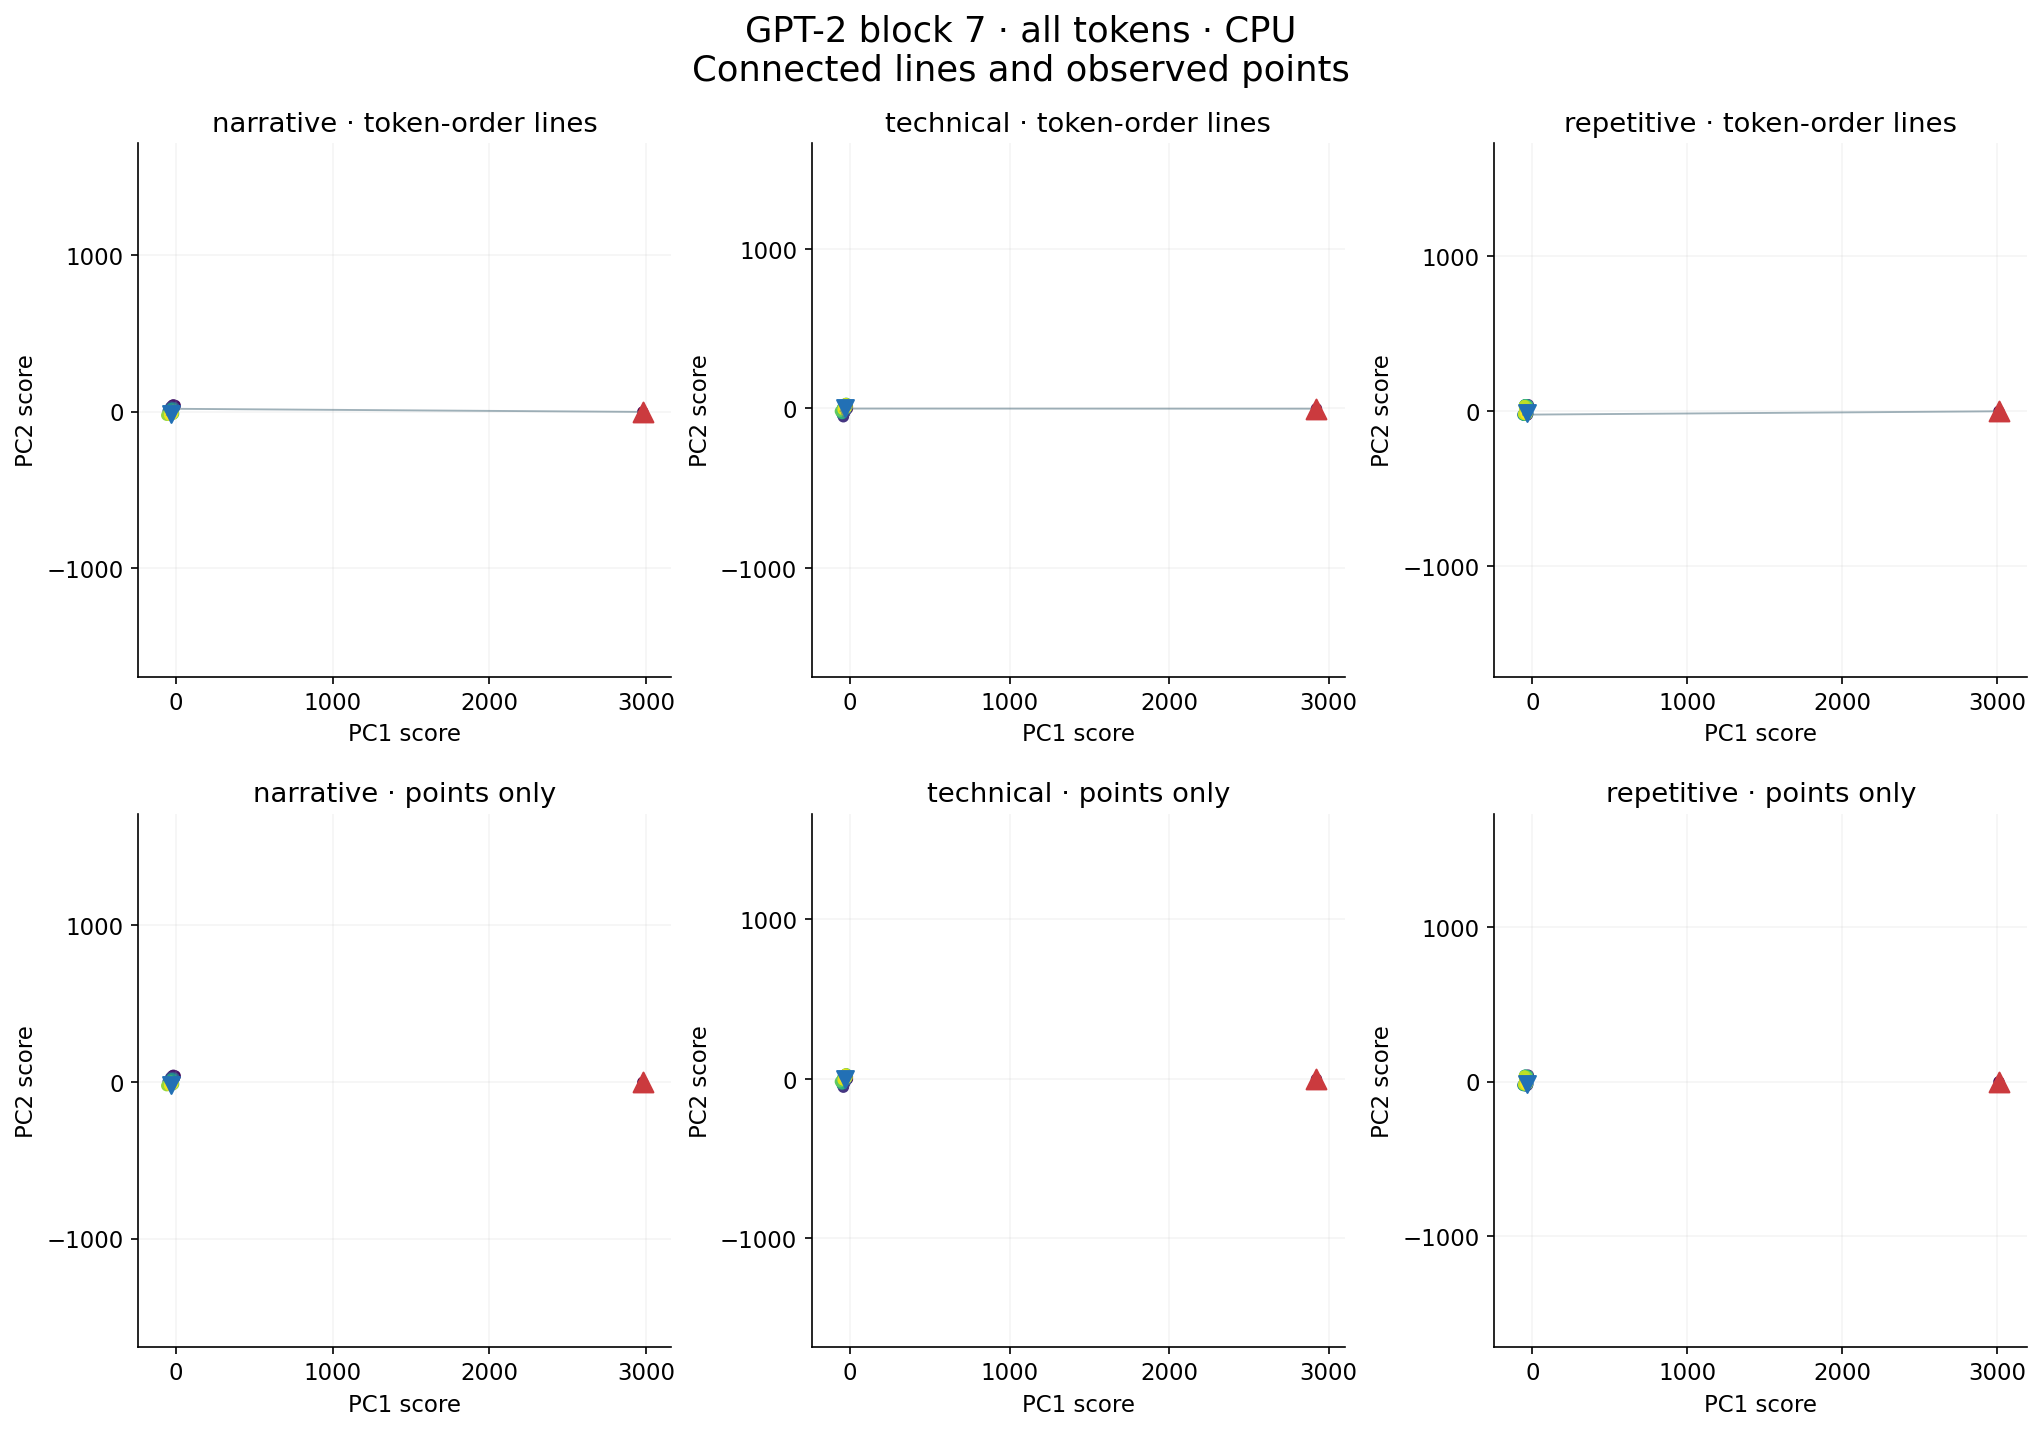
\includegraphics[width=\linewidth,height=0.73\textheight,keepaspectratio]{figures/01_short_text_points.png}
\captionof*{figure}{Figure 1. GPT-2 after block 7, CPU, all tokens. The top row connects adjacent tokens; the bottom row shows only the points at the same coordinates. Axes use equal scaling within each panel. Color indicates token order (purple to yellow); the red upward triangle marks the first token and the blue downward triangle the last. Lines are visual connections between observed points.}
\end{figure}

Point-distribution measurements supported this interpretation. The first token accounted for almost the entire PC1 sum of squares, with a large gap across the full PC1 range (Table 3). The strong association with the norm likewise arose in a configuration containing this distant point (Table C1). None of the three texts in the primary condition met the operational distribution-and-fit criterion defined in Section 2.6.

\Needspace{6\baselineskip}\begingroup
\fontsize{8.5}{11.2}\selectfont\setlength{\tabcolsep}{3pt}
{
\begin{longtable}[]{@{}
  >{\raggedright\arraybackslash}p{(\linewidth - 12\tabcolsep) * \real{0.1400}}
  >{\raggedleft\arraybackslash}p{(\linewidth - 12\tabcolsep) * \real{0.1300}}
  >{\raggedleft\arraybackslash}p{(\linewidth - 12\tabcolsep) * \real{0.1700}}
  >{\raggedleft\arraybackslash}p{(\linewidth - 12\tabcolsep) * \real{0.1300}}
  >{\raggedleft\arraybackslash}p{(\linewidth - 12\tabcolsep) * \real{0.1300}}
  >{\raggedleft\arraybackslash}p{(\linewidth - 12\tabcolsep) * \real{0.1500}}
  >{\raggedleft\arraybackslash}p{(\linewidth - 12\tabcolsep) * \real{0.1500}}@{}}
\caption*{\textbf{Table 3. Primary short-text conditions and sensitivity to the first token and norm.} CPU, after block 7. First-token PC1 contribution is its share of the centered PC1 sum of squares; maximum gap is relative to the full PC1 range. PCA was re-estimated for C1/C4.}\\
\toprule\noalign{}
\begin{minipage}[b]{\linewidth}\raggedright
Text
\end{minipage} & \begin{minipage}[b]{\linewidth}\raggedleft
All-point PC1 (\%)
\end{minipage} & \begin{minipage}[b]{\linewidth}\raggedleft
First-token PC1 contribution (\%)
\end{minipage} & \begin{minipage}[b]{\linewidth}\raggedleft
Maximum gap (\%)
\end{minipage} & \begin{minipage}[b]{\linewidth}\raggedleft
Occupied bins
\end{minipage} & \begin{minipage}[b]{\linewidth}\raggedleft
PC1 under C1 (\%)
\end{minipage} & \begin{minipage}[b]{\linewidth}\raggedleft
PC1 under C4 (\%)
\end{minipage} \\
\midrule\noalign{}
\endfirsthead
\caption*{\textbf{Table 3 (continued).}}\\
\toprule\noalign{}
\begin{minipage}[b]{\linewidth}\raggedright
Text
\end{minipage} & \begin{minipage}[b]{\linewidth}\raggedleft
All-point PC1 (\%)
\end{minipage} & \begin{minipage}[b]{\linewidth}\raggedleft
First-token PC1 contribution (\%)
\end{minipage} & \begin{minipage}[b]{\linewidth}\raggedleft
Maximum gap (\%)
\end{minipage} & \begin{minipage}[b]{\linewidth}\raggedleft
Occupied bins
\end{minipage} & \begin{minipage}[b]{\linewidth}\raggedleft
PC1 under C1 (\%)
\end{minipage} & \begin{minipage}[b]{\linewidth}\raggedleft
PC1 under C4 (\%)
\end{minipage} \\
\midrule\noalign{}
\endhead
\bottomrule\noalign{}
\endlastfoot
Narrative & 96.062 & 98.938 & 98.224 & 2/20 & 6.957 & 6.354 \\*
Technical & 96.571 & 98.768 & 98.524 & 2/20 & 7.380 & 7.009 \\*
Repetitive & 97.644 & 98.567 & 98.857 & 2/20 & 17.103 & 16.257 \\*
\end{longtable}
}
\endgroup

\FloatBarrier

\subsection{3.2 Excluding the first token and normalizing to unit length reveal the remaining variance structure}\label{excluding-the-first-token-and-normalizing-to-unit-length-reveal-the-remaining-variance-structure}

Excluding the first token from the analysis sharply reduced the extreme concentration in PC1. Normalizing each state to unit length before PCA reduced it to similar levels. Magnifying the all-point coordinates revealed variation within the dense cloud; recomputing PCA after excluding the first token redirected the principal axis toward variation within that cloud (Figure 2). Presenting these views together distinguishes magnification of the display from a change in which observations dominate the geometry.

\begin{figure}[!htbp]
\centering
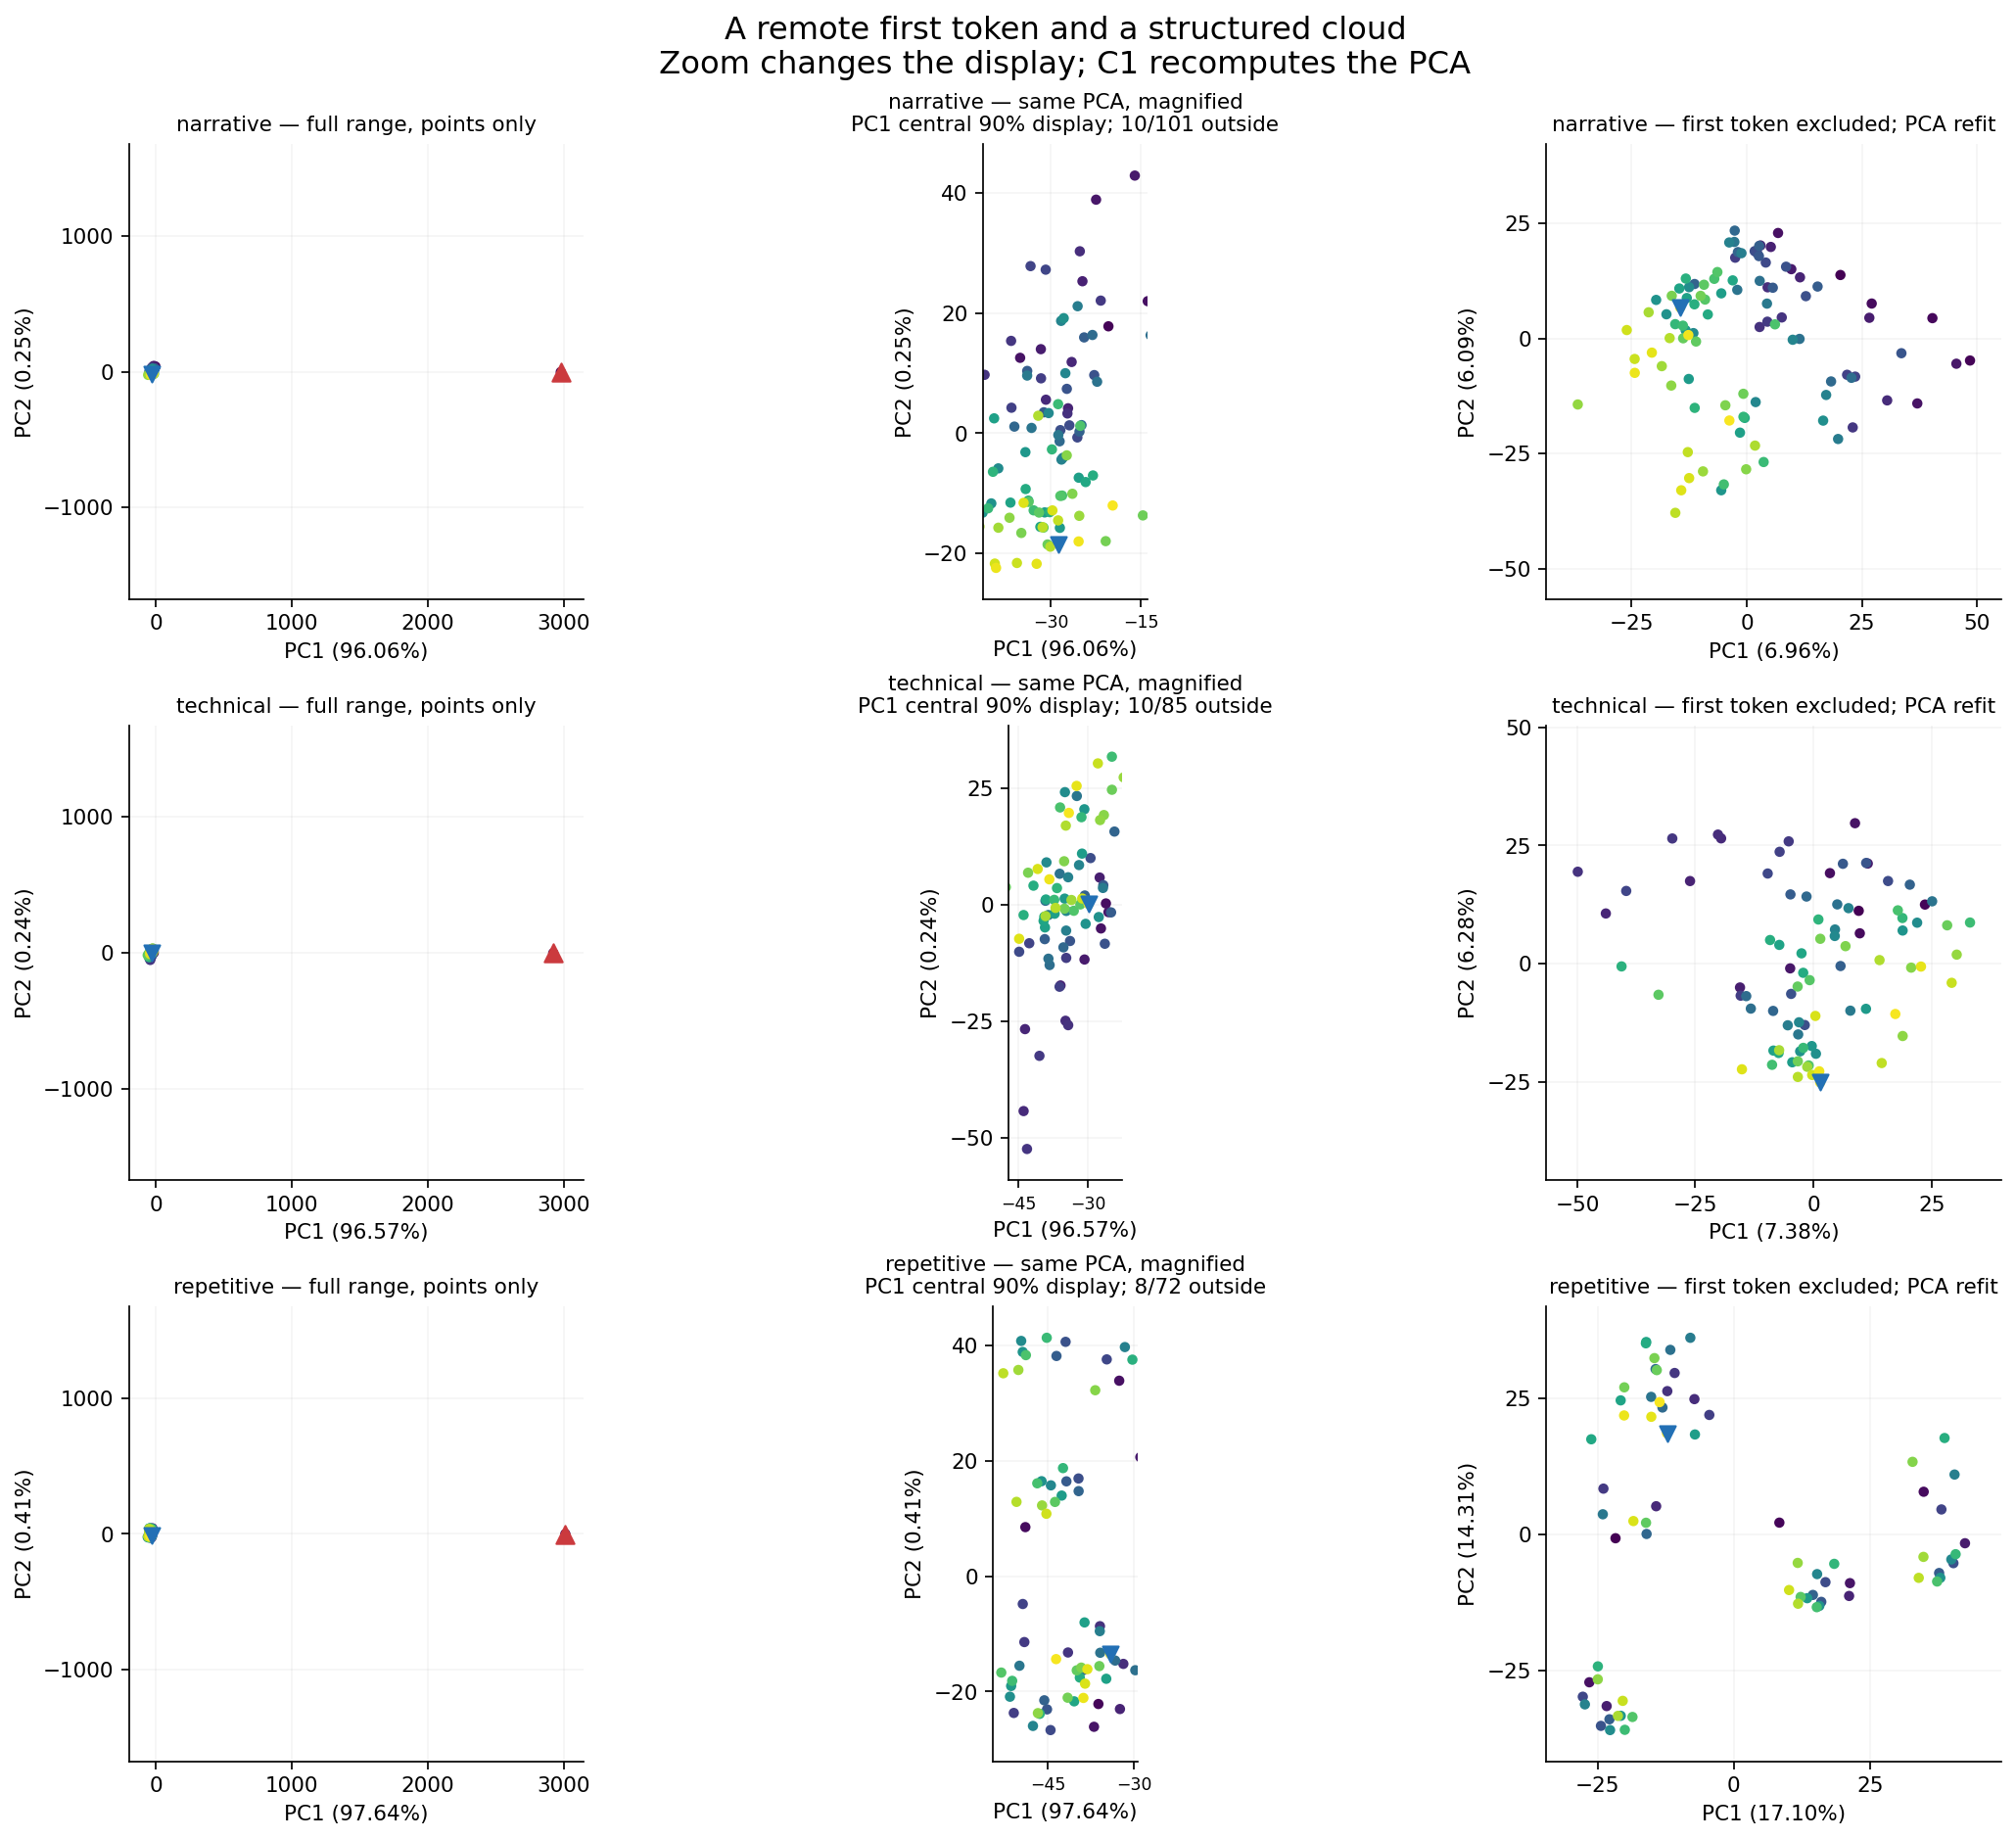
\includegraphics[width=\linewidth,height=0.73\textheight,keepaspectratio]{figures/02_short_text_sensitivity.png}
\captionof*{figure}{Figure 2. Full-range view of the primary condition (left), central 90\% of PC1 using the same PCA coordinates (center), and C1 with PCA re-estimated after excluding the first token (right). The center column leaves 10/101 narrative, 10/85 technical, and 8/72 repetitive points outside the displayed range; all points remain in the analysis. Axes use equal scaling within each panel.}
\end{figure}

A quadratic fitted to all points achieved high fit quality in the projected plane, but holding out contiguous blocks in position order produced large negative Q values (Table C1). Q has no finite lower bound: it is negative when the held-out squared error exceeds the total variation used as its denominator. Errors were concentrated at the first token. When the block containing that token was held out, the training points occupied a narrow range, and the fitted quadratic had to extrapolate to the distant first-token state. The large gap and unstable extrapolation show why a high all-point fit alone gives an incomplete description of the configuration.

\clearpage\begin{landscape}\thispagestyle{plain}
\subsection{3.3 Local residual coordinates contain feature associations that differ across texts}\label{local-residual-coordinates-contain-feature-associations-that-differ-across-texts}

Subtracting the quadratic mean trend along PC1 from PC2--8 in the primary condition left seven coordinates associated with position, decoded character length, and surprisal (Figure 3). The largest absolute position correlation occurred on residual PC2 in both the narrative and technical passages, and on residual PC5 in the repetitive passage. Token-level variation thus remained around the large axis dominated by the first token. These residual coordinates are defined separately for each text.
\vspace{5pt}

\centering
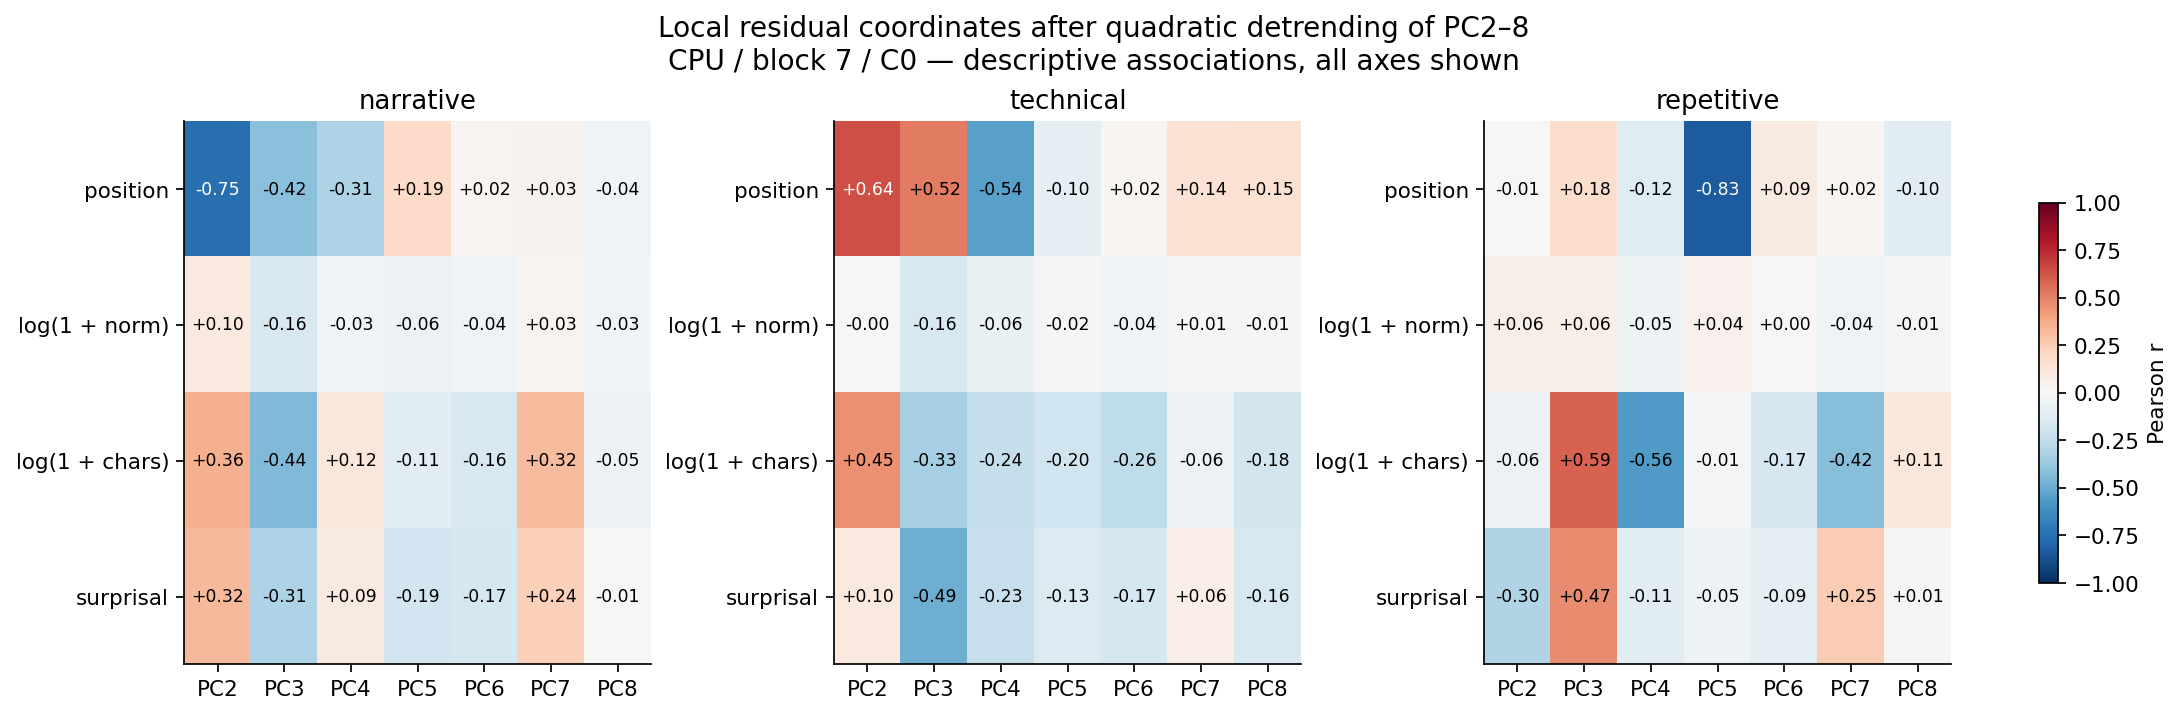
\includegraphics[width=\linewidth,height=0.74\textwidth,keepaspectratio]{figures/03_short_text_residuals.png}
\captionof*{figure}{Figure 3. Pearson correlations between seven local residual coordinates and four features in the primary condition. All axes and texts are shown. Norm and decoded character count are transformed as log(1 + value), as indicated by the row labels. The first position, where surprisal is undefined, is excluded from that correlation. Bases differ across texts; component indices and signs belong to each text's PCA.}
\end{landscape}

\FloatBarrier

\subsection{3.4 Curved configurations after final normalization depend on the input}\label{curved-configurations-after-final-normalization-depend-on-the-input}

For all three texts, PC1 concentration increased between the output of the final Transformer block and the state after the final LayerNorm. In the repetitive passage, adding a quadratic term yielded a larger improvement over a line on held-out blocks than in the narrative or technical passage, and the full-space fit was also strong (Table 4, Figure 4). The configuration therefore varied with both input and extraction point within the same model.

\Needspace{6\baselineskip}\begingroup
\fontsize{8.5}{11.2}\selectfont\setlength{\tabcolsep}{3pt}
{
\begin{longtable}[]{@{}
  >{\raggedright\arraybackslash}p{(\linewidth - 14\tabcolsep) * \real{0.1300}}
  >{\raggedleft\arraybackslash}p{(\linewidth - 14\tabcolsep) * \real{0.1300}}
  >{\raggedleft\arraybackslash}p{(\linewidth - 14\tabcolsep) * \real{0.1300}}
  >{\raggedleft\arraybackslash}p{(\linewidth - 14\tabcolsep) * \real{0.1200}}
  >{\raggedleft\arraybackslash}p{(\linewidth - 14\tabcolsep) * \real{0.1300}}
  >{\raggedleft\arraybackslash}p{(\linewidth - 14\tabcolsep) * \real{0.1400}}
  >{\raggedleft\arraybackslash}p{(\linewidth - 14\tabcolsep) * \real{0.1200}}
  >{\raggedleft\arraybackslash}p{(\linewidth - 14\tabcolsep) * \real{0.1000}}@{}}
\caption*{\textbf{Table 4. Variance concentration before and after final LayerNorm, and curve fits after it.} CPU, C0. Q uses 5 contiguous position-ordered folds. Gaps and occupancy are also measured after final LayerNorm.}\\
\toprule\noalign{}
\begin{minipage}[b]{\linewidth}\raggedright
Text
\end{minipage} & \begin{minipage}[b]{\linewidth}\raggedleft
PC1 before LN (\%)
\end{minipage} & \begin{minipage}[b]{\linewidth}\raggedleft
PC1 after LN (\%)
\end{minipage} & \begin{minipage}[b]{\linewidth}\raggedleft
Curve Q: 2D
\end{minipage} & \begin{minipage}[b]{\linewidth}\raggedleft
Curve Q: full space
\end{minipage} & \begin{minipage}[b]{\linewidth}\raggedleft
Curve − line Q: full space
\end{minipage} & \begin{minipage}[b]{\linewidth}\raggedleft
Maximum gap (\%)
\end{minipage} & \begin{minipage}[b]{\linewidth}\raggedleft
Occupied bins
\end{minipage} \\
\midrule\noalign{}
\endfirsthead
\caption*{\textbf{Table 4 (continued).}}\\
\toprule\noalign{}
\begin{minipage}[b]{\linewidth}\raggedright
Text
\end{minipage} & \begin{minipage}[b]{\linewidth}\raggedleft
PC1 before LN (\%)
\end{minipage} & \begin{minipage}[b]{\linewidth}\raggedleft
PC1 after LN (\%)
\end{minipage} & \begin{minipage}[b]{\linewidth}\raggedleft
Curve Q: 2D
\end{minipage} & \begin{minipage}[b]{\linewidth}\raggedleft
Curve Q: full space
\end{minipage} & \begin{minipage}[b]{\linewidth}\raggedleft
Curve − line Q: full space
\end{minipage} & \begin{minipage}[b]{\linewidth}\raggedleft
Maximum gap (\%)
\end{minipage} & \begin{minipage}[b]{\linewidth}\raggedleft
Occupied bins
\end{minipage} \\
\midrule\noalign{}
\endhead
\bottomrule\noalign{}
\endlastfoot
Narrative & 19.819 & 72.986 & 0.872 & 0.714 & +0.0043 & 14.618 & 16/20 \\*
Technical & 30.699 & 79.148 & 0.888 & 0.777 & +0.0041 & 18.698 & 17/20 \\*
Repetitive & 69.665 & 92.754 & 0.984 & 0.970 & +0.0517 & 21.525 & 13/20 \\*
\end{longtable}
}
\endgroup

\begin{figure}[!htbp]
\centering
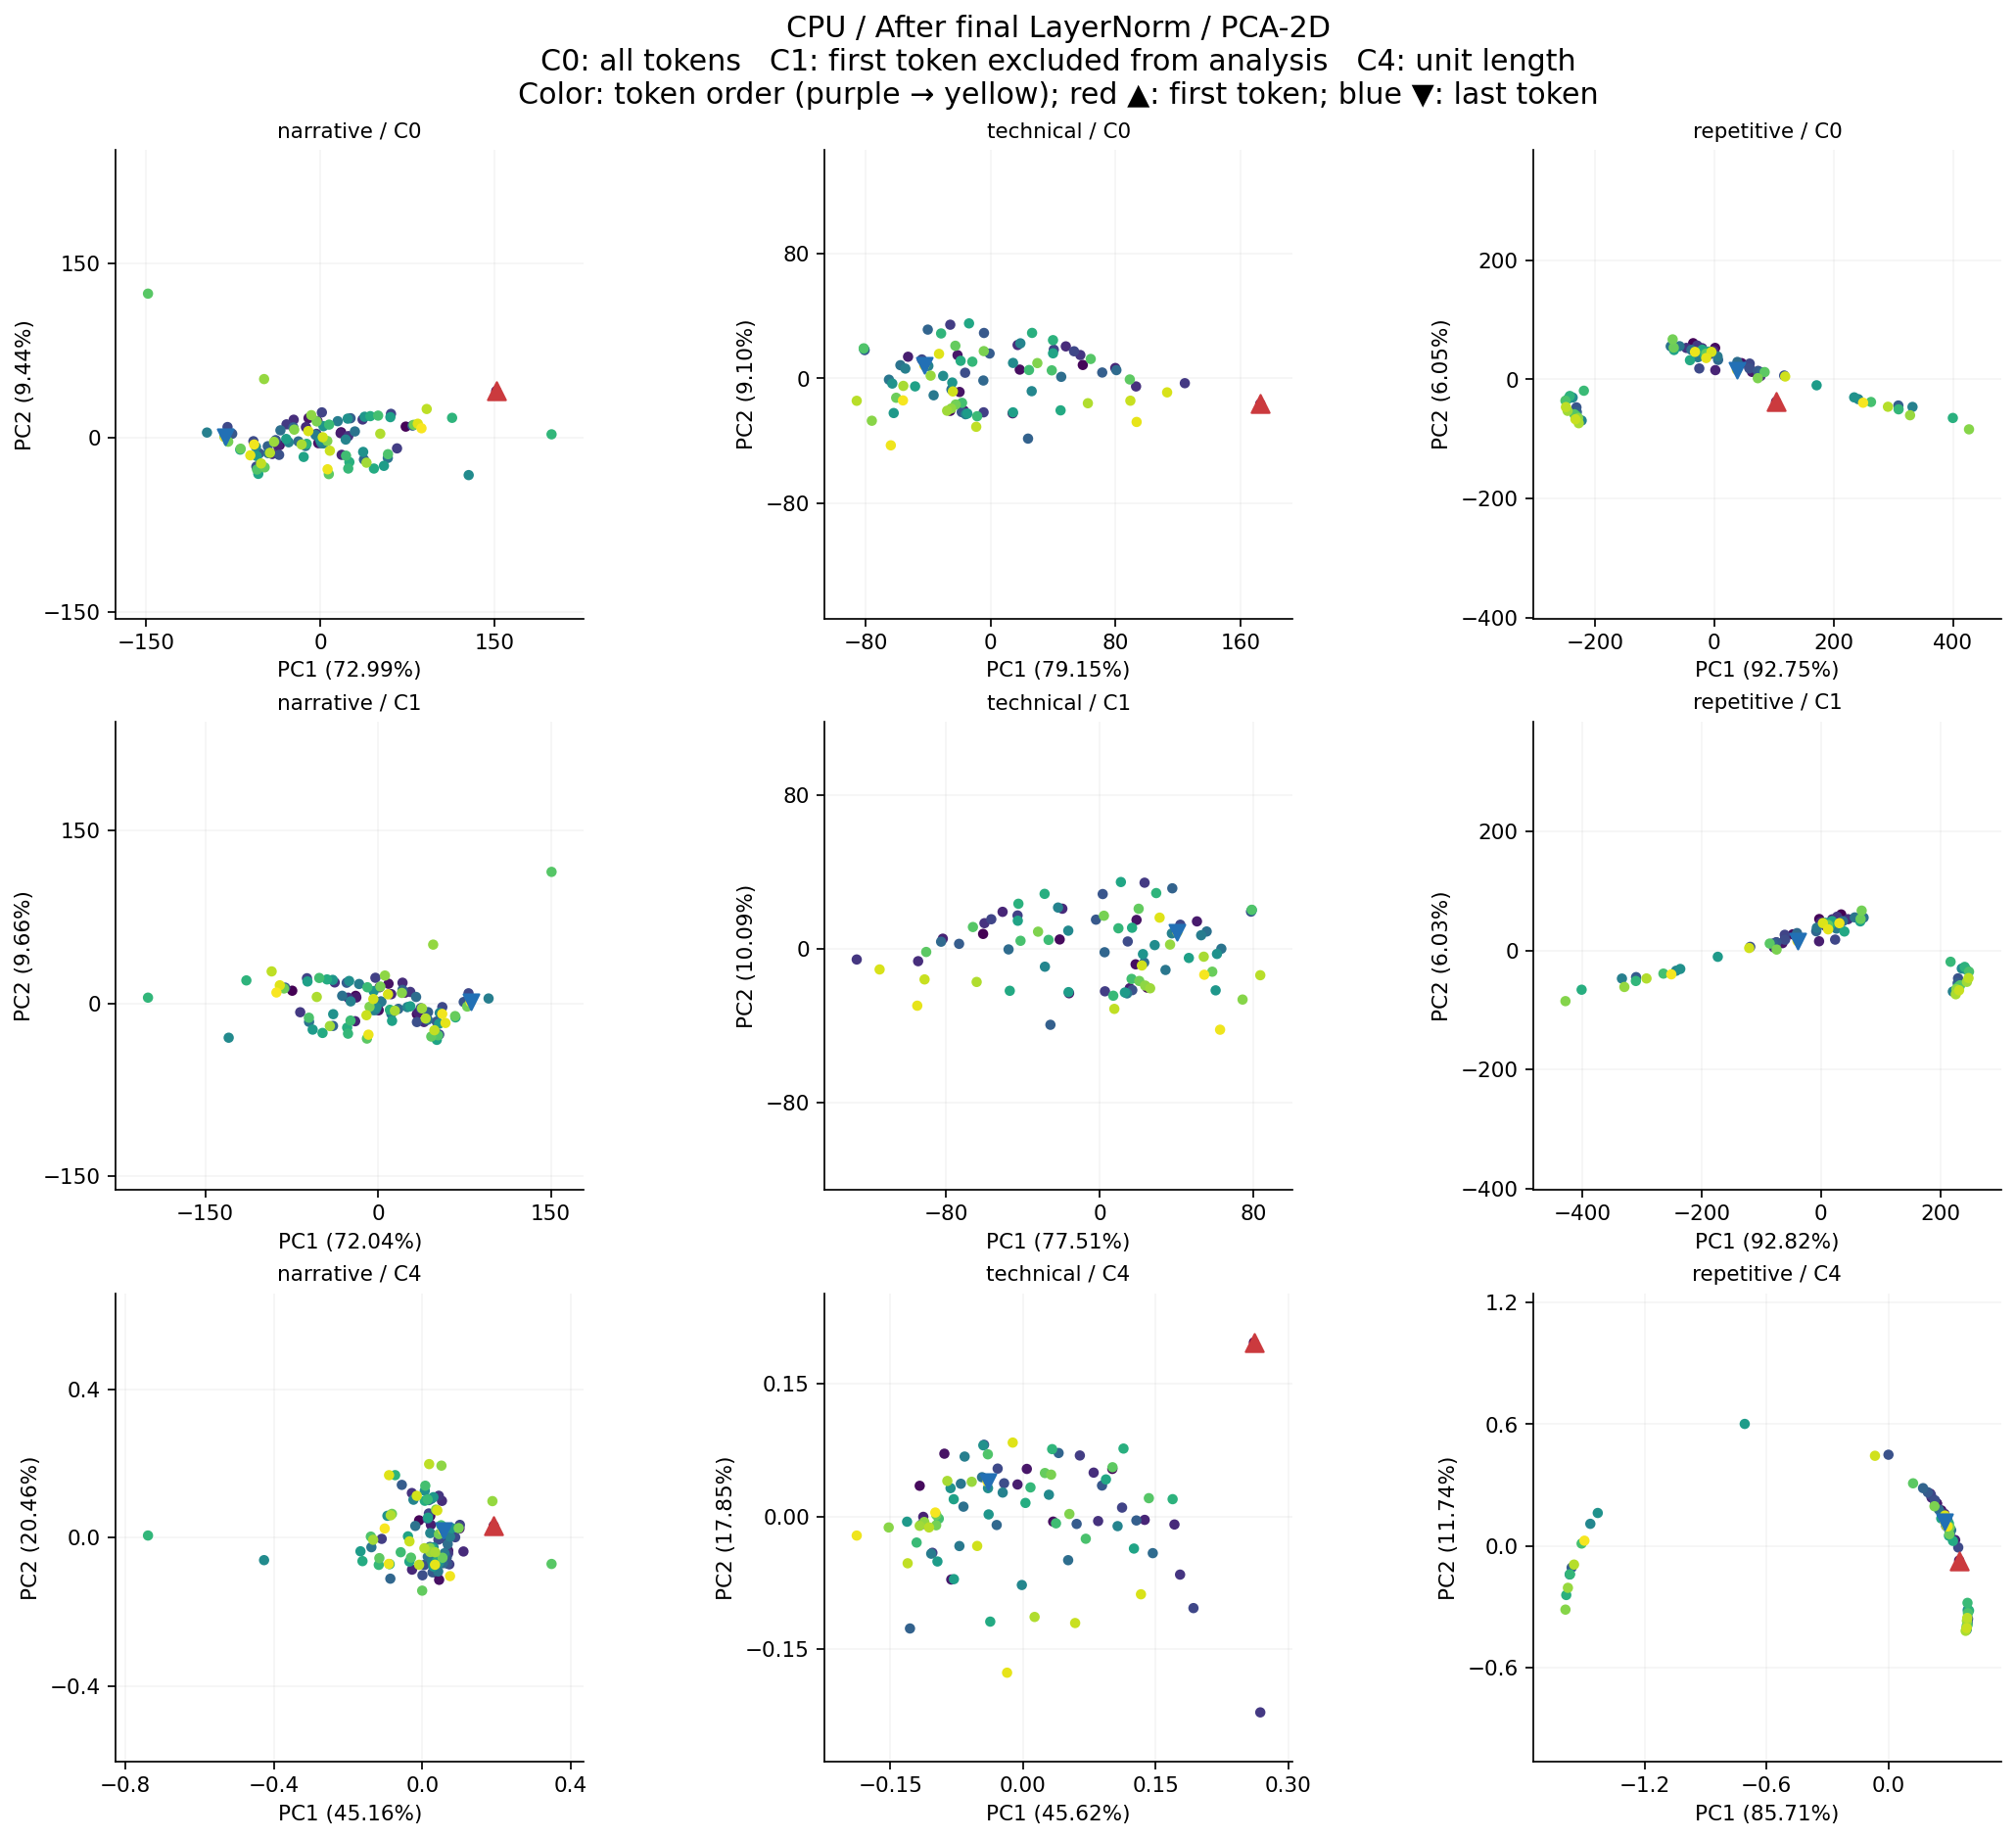
\includegraphics[width=\linewidth,height=0.73\textheight,keepaspectratio]{figures/04_short_text_final_ln.png}
\captionof*{figure}{Figure 4. GPT-2 after final LayerNorm, CPU. Columns show the narrative, technical, and repetitive passages; rows show C0/C1/C4. PCA is re-estimated for each condition, and all points use equal axis scaling. Color denotes token order (purple to yellow); the red upward triangle marks the first token and the blue downward triangle the last. C1 excludes the first token from analysis.}
\end{figure}

Although the repetitive passage had a good curve fit after final normalization, occupancy of 13/20 fell short of the 16/20 criterion, and its maximum gap of 21.525\% exceeded 10\%. Fit quality and the extent to which observations fill the full range are therefore distinct properties. The joint distribution-and-fit criterion was met in 0/3 primary conditions, 0/36 CPU conditions overall, and 0/36 GPU conditions. Section 6.6 presents the corresponding measurements for articles.

The results so far describe the observations that create each text's long axis and the feature associations found in its local residuals. Section 4 shifts the estimation scope to a training collection of articles, fixes the resulting shared basis and readout, and tests their incremental value on new articles.

\FloatBarrier

\section{4. Confirmatory results: from sensitivity of concentration to feature transfer}\label{confirmatory-results-from-sensitivity-of-concentration-to-feature-transfer}

\FloatBarrier

\subsection{4.1 The treatment of the first token strongly changes variance concentration}\label{the-treatment-of-the-first-token-strongly-changes-variance-concentration}

Our initial question was whether the strong PC1--norm correlation persisted as a pattern distributed throughout an article. At GPT-2's middle layer, excluding the first token sharply reduced both the norm correlation and the PC1 variance ratio. The first token had the largest norm in every article, and its treatment strongly affected the apparent geometry (Table 5, Figure 5; condition-specific levels appear in Table B1).

This result refuted the initial hypothesis that a high norm correlation would persist after excluding the first token. It also supported the hypothesis that excluding high-norm points would reduce concentration more than excluding the same number of points at random. Together, these findings establish sensitivity to high-norm points, including the first token, as central to interpreting the prominent middle-layer concentration.

\Needspace{6\baselineskip}\begingroup
\fontsize{9.3}{12}\selectfont\setlength{\tabcolsep}{3.3pt}
{
\begin{longtable}[]{@{}
  >{\raggedright\arraybackslash}p{(\linewidth - 4\tabcolsep) * \real{0.5100}}
  >{\raggedleft\arraybackslash}p{(\linewidth - 4\tabcolsep) * \real{0.1700}}
  >{\raggedright\arraybackslash}p{(\linewidth - 4\tabcolsep) * \real{0.3200}}@{}}
\caption*{\textbf{Table 5. Primary quantities in P1.} Each interval has level 98.333333\%. Differences in variance ratios are expressed as fractions.}\\
\toprule\noalign{}
\begin{minipage}[b]{\linewidth}\raggedright
Quantity
\end{minipage} & \begin{minipage}[b]{\linewidth}\raggedleft
Article median
\end{minipage} & \begin{minipage}[b]{\linewidth}\raggedright
Interval
\end{minipage} \\
\midrule\noalign{}
\endfirsthead
\caption*{\textbf{Table 5 (continued).}}\\
\toprule\noalign{}
\begin{minipage}[b]{\linewidth}\raggedright
Quantity
\end{minipage} & \begin{minipage}[b]{\linewidth}\raggedleft
Article median
\end{minipage} & \begin{minipage}[b]{\linewidth}\raggedright
Interval
\end{minipage} \\
\midrule\noalign{}
\endhead
\bottomrule\noalign{}
\endlastfoot
\(R_1\) after excluding the first token & 0.092305 & {[}0.075372, 0.142286{]} \\*
Paired difference in \(R_1\), C1−C0 & −0.905597 & {[}−0.922660, −0.855421{]} \\*
Paired difference in \(V_1\), C2−mean C3 & −0.753065 & {[}−0.755477, −0.749695{]} \\*
\end{longtable}
}
\endgroup

\clearpage\begin{landscape}\thispagestyle{plain}
\centering
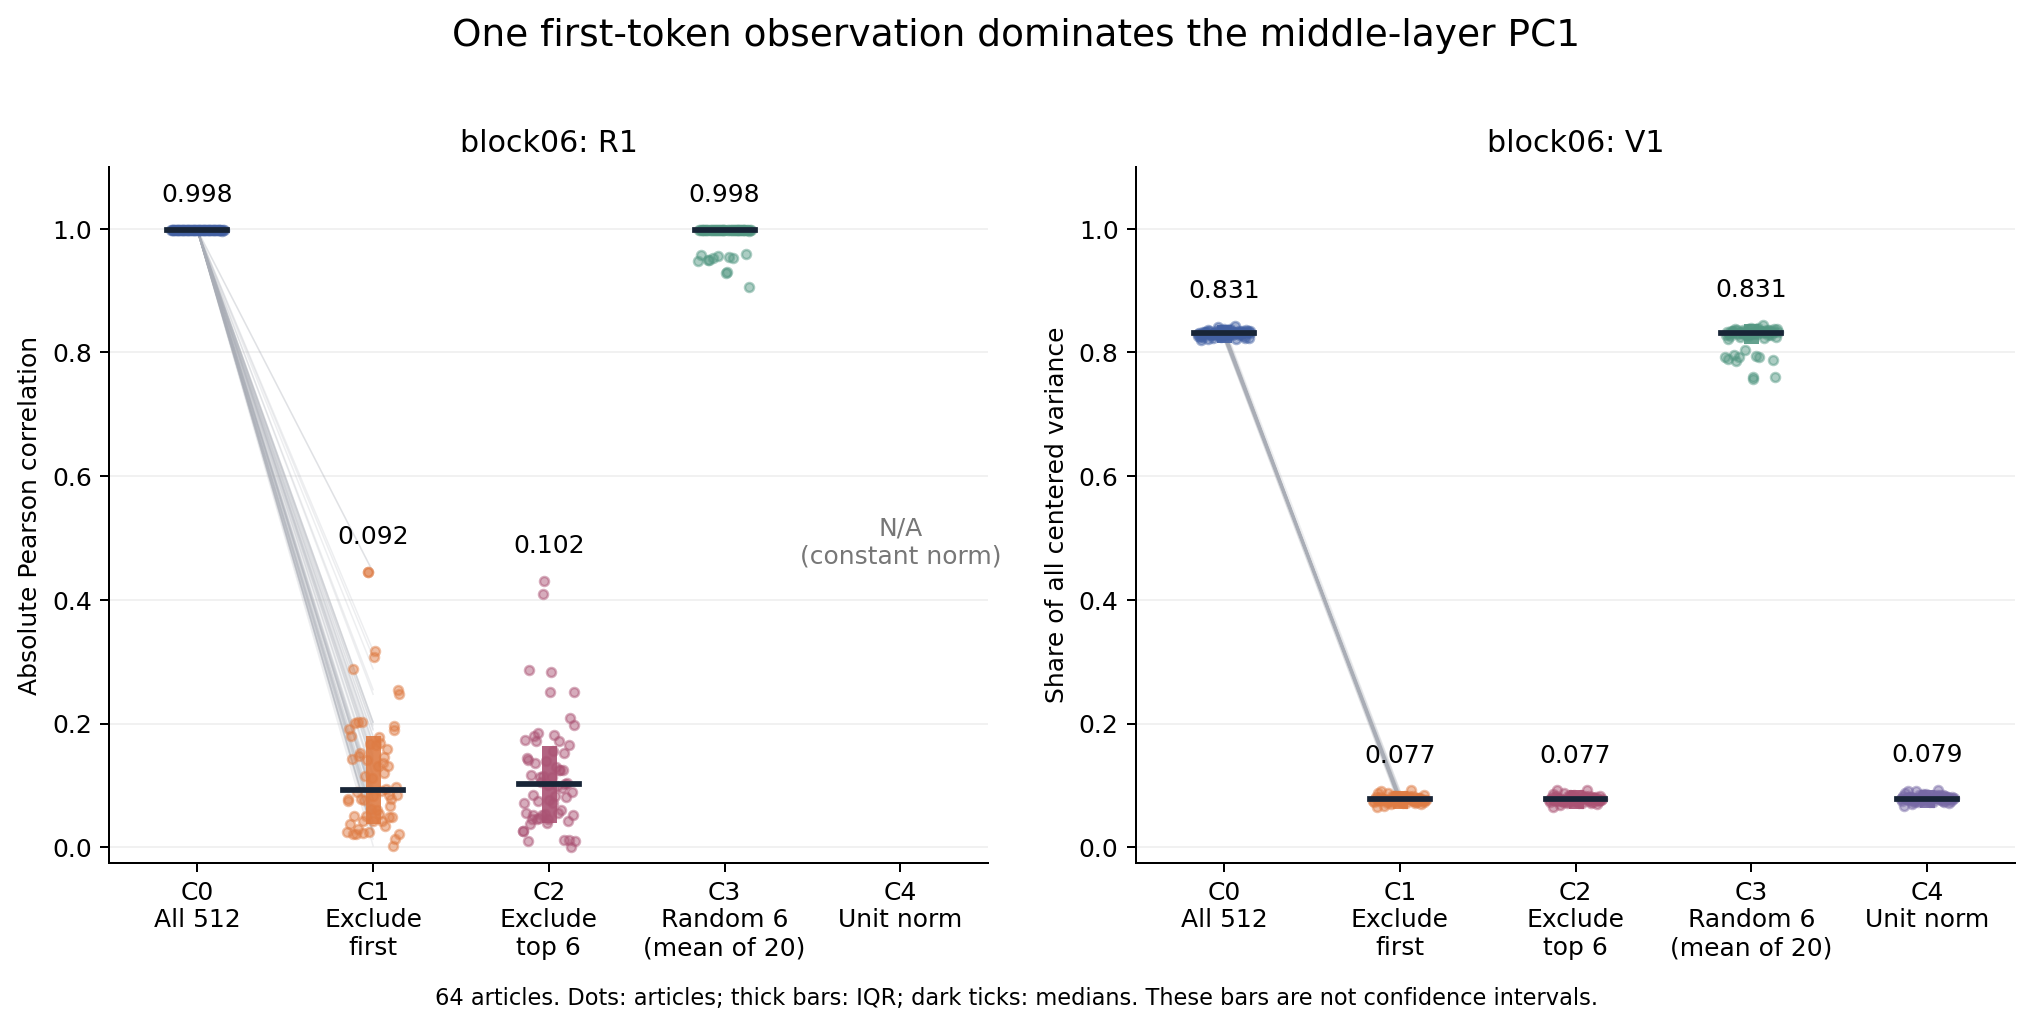
\includegraphics[width=\linewidth,height=0.74\textwidth,keepaspectratio]{figures/05_p1_first_token.png}
\captionof*{figure}{Figure 5. Conditions at the P1 middle layer. All 64 articles are shown; thick bars indicate interquartile ranges. C0--C3 comprise the comparisons for the primary hypotheses; C4 is a prespecified secondary description.}
\end{landscape}

\FloatBarrier

\subsection{4.2 Representations excluding the first token retain feature associations that transfer to separate articles}\label{representations-excluding-the-first-token-retain-feature-associations-that-transfer-to-separate-articles}

Given the dependence of concentration on the first token, we next examined which features could be read after excluding it. The center, basis, and readout were fixed on training articles and applied unchanged to separate articles.

The association with position persisted under transfer. Adding PCs to a baseline containing position, length, frequency, and norm also provided incremental readout of current-token surprisal. Both results met the prespecified criteria, including an advantage over random directions (Table 6). Thus, associations shared across articles remained after the first-token-sensitive concentration had weakened.

\Needspace{6\baselineskip}\begingroup
\fontsize{9.3}{12}\selectfont\setlength{\tabcolsep}{3.3pt}
{
\begin{longtable}[]{@{}
  >{\raggedright\arraybackslash}p{(\linewidth - 6\tabcolsep) * \real{0.4100}}
  >{\raggedleft\arraybackslash}p{(\linewidth - 6\tabcolsep) * \real{0.1600}}
  >{\raggedright\arraybackslash}p{(\linewidth - 6\tabcolsep) * \real{0.2500}}
  >{\raggedleft\arraybackslash}p{(\linewidth - 6\tabcolsep) * \real{0.1800}}@{}}
\caption*{\textbf{Table 6. Primary quantities for middle-layer C1 in P2.} Each interval has level 98.75\%.}\\
\toprule\noalign{}
\begin{minipage}[b]{\linewidth}\raggedright
Quantity
\end{minipage} & \begin{minipage}[b]{\linewidth}\raggedleft
Article median
\end{minipage} & \begin{minipage}[b]{\linewidth}\raggedright
Interval
\end{minipage} & \begin{minipage}[b]{\linewidth}\raggedleft
Lower bound required for support
\end{minipage} \\
\midrule\noalign{}
\endfirsthead
\caption*{\textbf{Table 6 (continued).}}\\
\toprule\noalign{}
\begin{minipage}[b]{\linewidth}\raggedright
Quantity
\end{minipage} & \begin{minipage}[b]{\linewidth}\raggedleft
Article median
\end{minipage} & \begin{minipage}[b]{\linewidth}\raggedright
Interval
\end{minipage} & \begin{minipage}[b]{\linewidth}\raggedleft
Lower bound required for support
\end{minipage} \\
\midrule\noalign{}
\endhead
\bottomrule\noalign{}
\endlastfoot
Position correlation with fixed sign & 0.786379 & {[}0.784334, 0.788167{]} & {\(\geq\)0.50} \\*
Position-correlation advantage over the random-set mean & 0.410946 & {[}0.405082, 0.417935{]} & {\(\geq\)0.10} \\*
PC increment for surprisal & 0.103522 & {[}0.088701, 0.114574{]} & {\(\geq\)0.02} \\*
Advantage over random directions for surprisal & 0.068226 & {[}0.057319, 0.081029{]} & {\(\geq\)0.01} \\*
\end{longtable}
}
\endgroup

\FloatBarrier

\subsection{4.3 Surprisal increments persist within recurring token IDs beyond lexical mean differences}\label{surprisal-increments-persist-within-recurring-token-ids-beyond-lexical-mean-differences}

Transfer to separate articles can still reflect average differences between token identities. We therefore fixed the lexical ID comparison model selected in an exploration of saved data and tested incremental value on new articles. In that exploration, the ID control was stronger than the nonlinear controls tested, and some PC increment remained after attenuation. Here we evaluate the conditions fixed in response to that comparison on articles not previously used in the study. Section 6.1 reports the full set of exploratory candidates.

At GPT-2's middle layer, the incremental value of PCs beyond the ID control persisted on separate articles. In a within-group evaluation comparing occurrences of the same ID in the same article, both the PC increment and the advantage over random directions also met the prespecified criteria (Table 7). Hidden states at individual occurrences thus supported readout of unexpectedness after removing mean differences between token identities. Table B3 gives article counts with positive and negative outcomes.

\Needspace{6\baselineskip}\begingroup
\fontsize{9.3}{12}\selectfont\setlength{\tabcolsep}{3.3pt}
{
\begin{longtable}[]{@{}
  >{\raggedright\arraybackslash}p{(\linewidth - 8\tabcolsep) * \real{0.1400}}
  >{\raggedright\arraybackslash}p{(\linewidth - 8\tabcolsep) * \real{0.2700}}
  >{\raggedleft\arraybackslash}p{(\linewidth - 8\tabcolsep) * \real{0.1400}}
  >{\raggedright\arraybackslash}p{(\linewidth - 8\tabcolsep) * \real{0.2700}}
  >{\raggedleft\arraybackslash}p{(\linewidth - 8\tabcolsep) * \real{0.1800}}@{}}
\caption*{\textbf{Table 7. Primary quantities for middle-layer C1 in P3.} Each interval has level 98.75\%.}\\
\toprule\noalign{}
\begin{minipage}[b]{\linewidth}\raggedright
Evaluation
\end{minipage} & \begin{minipage}[b]{\linewidth}\raggedright
Quantity
\end{minipage} & \begin{minipage}[b]{\linewidth}\raggedleft
Article median
\end{minipage} & \begin{minipage}[b]{\linewidth}\raggedright
Interval
\end{minipage} & \begin{minipage}[b]{\linewidth}\raggedleft
Lower bound required for support
\end{minipage} \\
\midrule\noalign{}
\endfirsthead
\caption*{\textbf{Table 7 (continued).}}\\
\toprule\noalign{}
\begin{minipage}[b]{\linewidth}\raggedright
Evaluation
\end{minipage} & \begin{minipage}[b]{\linewidth}\raggedright
Quantity
\end{minipage} & \begin{minipage}[b]{\linewidth}\raggedleft
Article median
\end{minipage} & \begin{minipage}[b]{\linewidth}\raggedright
Interval
\end{minipage} & \begin{minipage}[b]{\linewidth}\raggedleft
Lower bound required for support
\end{minipage} \\
\midrule\noalign{}
\endhead
\bottomrule\noalign{}
\endlastfoot
Ordinary & PC increment & 0.056019 & {[}0.049032, 0.061445{]} & {\(\geq\)0.02} \\*
Ordinary & Advantage over random directions & 0.028811 & {[}0.020351, 0.035687{]} & {\(\geq\)0.01} \\*
Within ID & PC increment & 0.033571 & {[}0.027323, 0.044717{]} & {\(\geq\)0.01} \\*
Within ID & Advantage over random directions & 0.015092 & {[}0.008209, 0.027739{]} & {\(\geq\)0.005} \\*
\end{longtable}
}
\endgroup

\FloatBarrier

\subsection{4.4 Support for within-group incremental value varies by model and extraction point}\label{support-for-within-group-incremental-value-varies-by-model-and-extraction-point}

Having found incremental surprisal readout within recurring token IDs, we extended the evaluation to multiple models using W, which directly learns within-group differences. On the known articles, restricting ordinary training to recurring IDs had already reversed the final-layer PC-versus-random ranking; within-group training increased the advantage further (Section 6.2). We fixed W and evaluated it using new training and evaluation articles.

The prespecified criteria were met after GPT-2's final normalization, at OPT's middle layer, and at both Qwen extraction points. GPT-2's middle layer and OPT's final normalized state were inconclusive because intervals crossed a minimum-effect threshold (Table 8, Figure 6). The training configuration changed from O in P3 to W in P4, and the training articles, evaluation articles, and interval levels also differed. For GPT-2's middle layer in P4, the PC increment met its criterion, but the lower bound of the advantage over random directions did not, resulting in an inconclusive outcome. Overall, four conditions met both support criteria and two were inconclusive; the criterion requiring support across all 6 conditions was not met. These decisions concern whether each condition meets its specified minimum effects. Table 8b reports absolute performance. Evaluation included tokens belonging to IDs that recur within the same article: for GPT-2, for example, this comprised 20,522 of the 31,017 C1 tokens across all 64 articles.

\Needspace{6\baselineskip}\begingroup
\fontsize{9.3}{12}\selectfont\setlength{\tabcolsep}{3.3pt}
{
\begin{longtable}[]{@{}
  >{\raggedright\arraybackslash}p{(\linewidth - 6\tabcolsep) * \real{0.2500}}
  >{\raggedright\arraybackslash}p{(\linewidth - 6\tabcolsep) * \real{0.2900}}
  >{\raggedright\arraybackslash}p{(\linewidth - 6\tabcolsep) * \real{0.3000}}
  >{\raggedright\arraybackslash}p{(\linewidth - 6\tabcolsep) * \real{0.1600}}@{}}
\caption*{\textbf{Table 8. Confirmatory results in P4.} All conditions use C1 and within-group evaluation with W, with 64 articles each. Interval level: 99.583333\%. Support requires both a PC-increment lower bound \textgreater.01 and an advantage lower bound \textgreater.005.}\\
\toprule\noalign{}
\begin{minipage}[b]{\linewidth}\raggedright
Model and extraction point
\end{minipage} & \begin{minipage}[b]{\linewidth}\raggedright
PC increment {[}interval{]}
\end{minipage} & \begin{minipage}[b]{\linewidth}\raggedright
Advantage over random directions {[}interval{]}
\end{minipage} & \begin{minipage}[b]{\linewidth}\raggedright
Composite decision
\end{minipage} \\
\midrule\noalign{}
\endfirsthead
\caption*{\textbf{Table 8 (continued).}}\\
\toprule\noalign{}
\begin{minipage}[b]{\linewidth}\raggedright
Model and extraction point
\end{minipage} & \begin{minipage}[b]{\linewidth}\raggedright
PC increment {[}interval{]}
\end{minipage} & \begin{minipage}[b]{\linewidth}\raggedright
Advantage over random directions {[}interval{]}
\end{minipage} & \begin{minipage}[b]{\linewidth}\raggedright
Composite decision
\end{minipage} \\
\midrule\noalign{}
\endhead
\bottomrule\noalign{}
\endlastfoot
GPT-2 middle & 0.035549 {[}0.024553, 0.052815{]} & 0.014655 {[}0.000167, 0.028367{]} & Inconclusive \\*
GPT-2 after final LayerNorm & 0.097713 {[}0.083537, 0.121231{]} & 0.016303 {[}0.012567, 0.023536{]} & Supported \\*
OPT-1.3B middle & 0.049142 {[}0.033490, 0.062793{]} & 0.029996 {[}0.014675, 0.044107{]} & Supported \\*
OPT-1.3B after final LayerNorm & 0.015561 {[}0.008232, 0.022705{]} & 0.008795 {[}0.001584, 0.017265{]} & Inconclusive \\*
Qwen2.5-1.5B middle & 0.070771 {[}0.051705, 0.088018{]} & 0.040772 {[}0.028871, 0.052625{]} & Supported \\*
Qwen2.5-1.5B after final RMSNorm & 0.022240 {[}0.015933, 0.035083{]} & 0.011978 {[}0.005662, 0.026762{]} & Supported \\*
\end{longtable}
}
\endgroup

\Needspace{6\baselineskip}\begingroup
\fontsize{9.3}{12}\selectfont\setlength{\tabcolsep}{3.3pt}
{
\begin{longtable}[]{@{}
  >{\raggedright\arraybackslash}p{(\linewidth - 6\tabcolsep) * \real{0.4000}}
  >{\raggedleft\arraybackslash}p{(\linewidth - 6\tabcolsep) * \real{0.1800}}
  >{\raggedleft\arraybackslash}p{(\linewidth - 6\tabcolsep) * \real{0.1900}}
  >{\raggedleft\arraybackslash}p{(\linewidth - 6\tabcolsep) * \real{0.2300}}@{}}
\caption*{\textbf{Table 8b. Absolute {R\textsuperscript{2}} for W in P4.} All conditions use C1; values are medians across 64 articles. The random column is the median of each article's mean over 20 random sets. Differences between medians need not equal the median of article-level increments in Table 8.}\\
\toprule\noalign{}
\begin{minipage}[b]{\linewidth}\raggedright
Model and extraction point
\end{minipage} & \begin{minipage}[b]{\linewidth}\raggedleft
Baseline {R\textsuperscript{2}}
\end{minipage} & \begin{minipage}[b]{\linewidth}\raggedleft
{R\textsuperscript{2}} with PCs
\end{minipage} & \begin{minipage}[b]{\linewidth}\raggedleft
{R\textsuperscript{2}} with random directions
\end{minipage} \\
\midrule\noalign{}
\endfirsthead
\caption*{\textbf{Table 8b (continued).}}\\
\toprule\noalign{}
\begin{minipage}[b]{\linewidth}\raggedright
Model and extraction point
\end{minipage} & \begin{minipage}[b]{\linewidth}\raggedleft
Baseline {R\textsuperscript{2}}
\end{minipage} & \begin{minipage}[b]{\linewidth}\raggedleft
{R\textsuperscript{2}} with PCs
\end{minipage} & \begin{minipage}[b]{\linewidth}\raggedleft
{R\textsuperscript{2}} with random directions
\end{minipage} \\
\midrule\noalign{}
\endhead
\bottomrule\noalign{}
\endlastfoot
GPT-2 middle & 0.176547 & 0.213594 & 0.200651 \\*
GPT-2 after final normalization & 0.113743 & 0.216020 & 0.194298 \\*
OPT middle & 0.095358 & 0.142168 & 0.118050 \\*
OPT after final normalization & 0.107015 & 0.123989 & 0.116116 \\*
Qwen middle & 0.063325 & 0.135736 & 0.093081 \\*
Qwen after final normalization & 0.070855 & 0.098147 & 0.082759 \\*
\end{longtable}
}
\endgroup

These decisions concern increments for a typical article. Stability across all articles also requires examining the distribution. At Qwen's middle layer, a failure makes the mean article-level increment negative (Section 6.5).

\clearpage\begin{landscape}\thispagestyle{plain}
\centering
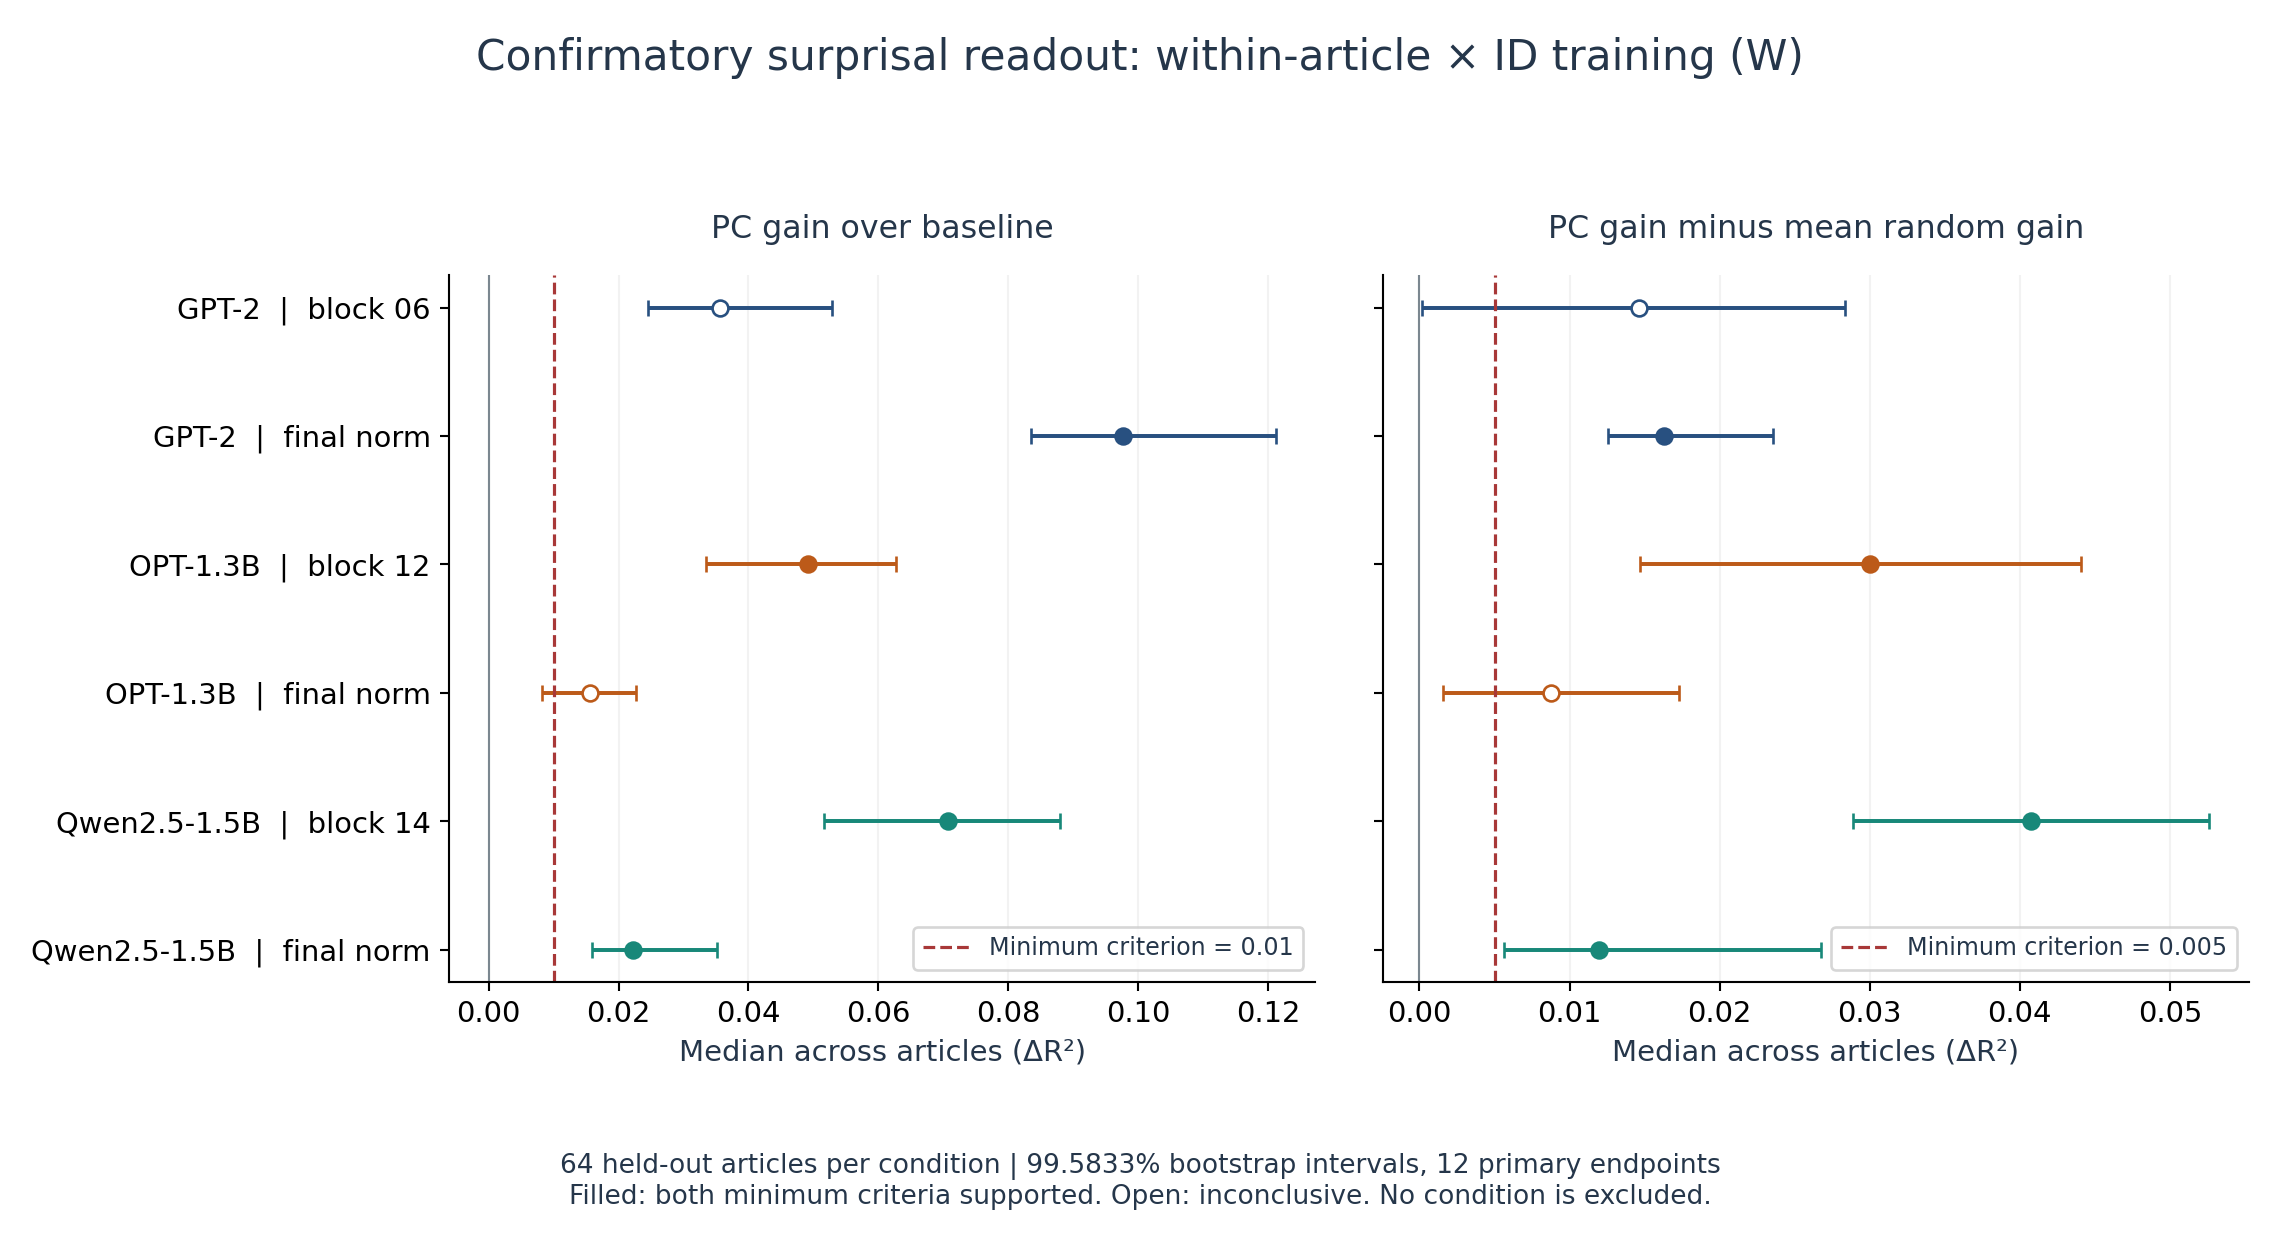
\includegraphics[width=\linewidth,height=0.74\textwidth,keepaspectratio]{figures/06_p4_confirmatory.png}
\captionof*{figure}{Figure 6. Confirmatory within-article × ID surprisal results in P4, using recurring IDs and W training. Points are medians across articles, bars are 99.583333\% intervals, and dashed lines are the prespecified minimum effects. Filled points denote conditions meeting both criteria; open points denote inconclusive conditions. All 6 conditions are shown.}
\end{landscape}

\FloatBarrier

\section{5. Prespecified secondary descriptions: concentration and readout need not follow the same pattern}\label{prespecified-secondary-descriptions-concentration-and-readout-need-not-follow-the-same-pattern}

\FloatBarrier

\subsection{5.1 First-token sensitivity and final-layer concentration show different patterns}\label{first-token-sensitivity-and-final-layer-concentration-show-different-patterns}

Examining the confirmatory results across extraction layers revealed that sensitivity to the first token was not uniform. After GPT-2's final LayerNorm, strong concentration persisted after excluding the first token and after normalization to unit length. The same model thus exhibited both substantial first-token dependence at the middle layer and persistent concentration at the final layer.

Across models, first-token sensitivity at the middle layer and concentration at the final layer appeared in different combinations. Excluding the first token sharply reduced the middle-layer variance ratio in GPT-2 and Qwen, whereas the change was smaller in OPT. The concentration remaining after final normalization also differed across models (Table B1). These observations show why both model and extraction layer must be specified when interpreting variance concentration.

\FloatBarrier

\subsection{5.2 The feature being read changes the assessment of the same geometry}\label{the-feature-being-read-changes-the-assessment-of-the-same-geometry}

At the middle layer, the association with position transferred to separate articles for bases fitted under different preprocessing conditions. PC2 was selected as the position-related direction when all points were used, whereas PC1 was selected after excluding the first token or normalizing states to unit length. After final LayerNorm, in contrast, transfer of the position direction was weak, while incremental surprisal readout was positive (Table B2). The assessment of the same extraction layer therefore depended on the target feature.

The choice of comparator also mattered. In the within-group evaluation after final LayerNorm using the fixed ID control, adding PCs improved performance but fell below the average performance of random directions (Table B3). This reversal motivated an examination of the relationship between the variation concentrated in PCs and what the predictor was trained to learn. The next section diagnoses these candidate explanations using saved data.

\FloatBarrier

\section{6. Exploratory analyses: where incremental value resides and how readout conditions matter}\label{exploratory-analyses-where-incremental-value-resides-and-how-readout-conditions-matter}

The preceding results showed that readout performance varied with lexical controls and extraction layers. Here we use saved data to examine candidate explanations for those differences. Computational conditions were recorded before each exploratory analysis, and all candidates and conditions were retained. Outcomes on the evaluation articles were already known; the intervals below are exploratory descriptive intervals.

\FloatBarrier

\subsection{6.1 Lexical controls attenuate the increment, while leaving a residual gain}\label{lexical-controls-attenuate-the-increment-while-leaving-a-residual-gain}

As a first step toward understanding the incremental value of PCs, we assessed how well the baseline captured lexical differences. We compared an ID model adding token-ID effects to the original features, an NL model adding nonlinear terms, interactions, and character-shape features, and a model combining both.

The ID model was the strongest comparator in both training-set cross-validation and baseline performance on evaluation articles. Introducing this control reduced the PC increment relative to the original comparison, but incremental value and an advantage over random directions remained (Table 9; intervals in Table B3). This motivated fixing the comparison model, including its coefficients, and testing it on new articles in the confirmation reported in Section 4.3.

\Needspace{6\baselineskip}\begingroup
\fontsize{9.3}{12}\selectfont\setlength{\tabcolsep}{3.3pt}
{
\begin{longtable}[]{@{}
  >{\raggedright\arraybackslash}p{(\linewidth - 8\tabcolsep) * \real{0.1900}}
  >{\raggedleft\arraybackslash}p{(\linewidth - 8\tabcolsep) * \real{0.1600}}
  >{\raggedleft\arraybackslash}p{(\linewidth - 8\tabcolsep) * \real{0.1800}}
  >{\raggedleft\arraybackslash}p{(\linewidth - 8\tabcolsep) * \real{0.2000}}
  >{\raggedleft\arraybackslash}p{(\linewidth - 8\tabcolsep) * \real{0.2700}}@{}}
\caption*{\textbf{Table 9. Exploratory strengthening of controls for middle-layer C1 in P2.} Medians across 64 articles.}\\
\toprule\noalign{}
\begin{minipage}[b]{\linewidth}\raggedright
Baseline model
\end{minipage} & \begin{minipage}[b]{\linewidth}\raggedleft
Baseline {R\textsuperscript{2}}
\end{minipage} & \begin{minipage}[b]{\linewidth}\raggedleft
{R\textsuperscript{2}} with PCs
\end{minipage} & \begin{minipage}[b]{\linewidth}\raggedleft
PC increment
\end{minipage} & \begin{minipage}[b]{\linewidth}\raggedleft
Advantage over random directions
\end{minipage} \\
\midrule\noalign{}
\endfirsthead
\caption*{\textbf{Table 9 (continued).}}\\
\toprule\noalign{}
\begin{minipage}[b]{\linewidth}\raggedright
Baseline model
\end{minipage} & \begin{minipage}[b]{\linewidth}\raggedleft
Baseline {R\textsuperscript{2}}
\end{minipage} & \begin{minipage}[b]{\linewidth}\raggedleft
{R\textsuperscript{2}} with PCs
\end{minipage} & \begin{minipage}[b]{\linewidth}\raggedleft
PC increment
\end{minipage} & \begin{minipage}[b]{\linewidth}\raggedleft
Advantage over random directions
\end{minipage} \\
\midrule\noalign{}
\endhead
\bottomrule\noalign{}
\endlastfoot
Original P2 & 0.144247 & 0.252093 & 0.103522 & 0.068226 \\*
ID & 0.280944 & 0.339169 & 0.050095 & 0.028559 \\*
NL & 0.093 & 0.171 & 0.0658 & 0.0295 \\*
NL ID & 0.172 & 0.232 & 0.0579 & 0.0165 \\*
\end{longtable}
}
\endgroup

Models with many nonlinear features performed worse than the ID model, separating complexity from actual strength as a comparator.

\FloatBarrier

\subsection{6.2 The final-layer reversal changes with the readout training configuration}\label{the-final-layer-reversal-changes-with-the-readout-training-configuration}

We examined the final-layer reversal by changing the training population and then the objective. Starting from the original predictor O, we compared ordinary training restricted to recurring IDs (R), training on within-group deviations with the same tokens and penalties (W fixed), and within-group training with its own penalty selection (W CV).

Restricting ordinary training to recurring IDs already reversed the median PC-versus-random ranking. Training on within-group deviations increased the advantage further, including with penalties fixed, and favored PCs on most articles (Table 10; article counts in Table B3). The shared top 8 components captured most within-group state variation. In this comparison, the value of that concentrated variation for readout depended on both the training tokens and the objective.

\Needspace{6\baselineskip}\begingroup
\fontsize{9.3}{12}\selectfont\setlength{\tabcolsep}{3.3pt}
{
\begin{longtable}[]{@{}
  >{\raggedright\arraybackslash}p{(\linewidth - 4\tabcolsep) * \real{0.4000}}
  >{\raggedleft\arraybackslash}p{(\linewidth - 4\tabcolsep) * \real{0.1900}}
  >{\raggedright\arraybackslash}p{(\linewidth - 4\tabcolsep) * \real{0.4100}}@{}}
\caption*{\textbf{Table 10. Within-group evaluation after GPT-2's final LayerNorm.} Exploratory; 64 articles per configuration. Advantages include descriptive 95\% intervals.}\\
\toprule\noalign{}
\begin{minipage}[b]{\linewidth}\raggedright
Configuration
\end{minipage} & \begin{minipage}[b]{\linewidth}\raggedleft
PC increment
\end{minipage} & \begin{minipage}[b]{\linewidth}\raggedright
Advantage over random directions {[}95\% interval{]}
\end{minipage} \\
\midrule\noalign{}
\endfirsthead
\caption*{\textbf{Table 10 (continued).}}\\
\toprule\noalign{}
\begin{minipage}[b]{\linewidth}\raggedright
Configuration
\end{minipage} & \begin{minipage}[b]{\linewidth}\raggedleft
PC increment
\end{minipage} & \begin{minipage}[b]{\linewidth}\raggedright
Advantage over random directions {[}95\% interval{]}
\end{minipage} \\
\midrule\noalign{}
\endhead
\bottomrule\noalign{}
\endlastfoot
O: original fixed predictor & 0.082171 & −0.009382 {[}−0.017125, −0.006356{]} \\*
R: ordinary training on recurring IDs & 0.098983 & 0.006024 {[}0.002833, 0.008507{]} \\*
W fixed: within-group training, fixed penalties & 0.119838 & 0.017109 {[}0.012541, 0.020310{]} \\*
W CV: within-group training, training-set tuning & 0.122506 & 0.018916 {[}0.014456, 0.020597{]} \\*
\end{longtable}
}
\endgroup

We carried the within-group objective into the subsequent confirmation. The result after GPT-2's final normalization in Section 4.4 shows that this configuration, selected through exploration, met its fixed criteria on new articles.

\FloatBarrier

\subsection{6.3 Much of the incremental value after controlling for position and vector norm resides in PC2--8}\label{much-of-the-incremental-value-after-controlling-for-position-and-vector-norm-resides-in-pc28}

We next examined which components support useful readout. We split the shared basis into PC1, PC2--8, and all 8 components and added each subset to a baseline accounting for position and log1p norm. Each subset was paired with a random control of the same dimensionality.

PC2--8 provided incremental value and an advantage over random directions in every condition examined. PC1 alone contributed little in many conditions, with a clearer increment at OPT's middle layer (Table 11; supplementary values in Table B3). For readouts already accounting for position and vector norm, PC2--8 formed a useful group of components for reading additional associations.

\Needspace{6\baselineskip}\begingroup
\fontsize{9.3}{12}\selectfont\setlength{\tabcolsep}{3.3pt}
{
\begin{longtable}[]{@{}
  >{\raggedright\arraybackslash}p{(\linewidth - 8\tabcolsep) * \real{0.1900}}
  >{\raggedleft\arraybackslash}p{(\linewidth - 8\tabcolsep) * \real{0.1200}}
  >{\raggedright\arraybackslash}p{(\linewidth - 8\tabcolsep) * \real{0.2700}}
  >{\raggedright\arraybackslash}p{(\linewidth - 8\tabcolsep) * \real{0.2900}}
  >{\raggedleft\arraybackslash}p{(\linewidth - 8\tabcolsep) * \real{0.1300}}@{}}
\caption*{\textbf{Table 11. Exploratory increments and control comparisons for PC subsets.} Medians across 64 articles. The PC2--8 increment and its advantage over random directions include unadjusted descriptive 95\% intervals. The comparator for the advantage is the mean over 20 sets of random orthogonal directions matched at 7 dimensions.}\\
\toprule\noalign{}
\begin{minipage}[b]{\linewidth}\raggedright
Condition
\end{minipage} & \begin{minipage}[b]{\linewidth}\raggedleft
PC1 increment
\end{minipage} & \begin{minipage}[b]{\linewidth}\raggedright
PC2--8 increment {[}95\% interval{]}
\end{minipage} & \begin{minipage}[b]{\linewidth}\raggedright
PC2--8 advantage over random directions {[}95\% interval{]}
\end{minipage} & \begin{minipage}[b]{\linewidth}\raggedleft
PC1--8 increment
\end{minipage} \\
\midrule\noalign{}
\endfirsthead
\caption*{\textbf{Table 11 (continued).}}\\
\toprule\noalign{}
\begin{minipage}[b]{\linewidth}\raggedright
Condition
\end{minipage} & \begin{minipage}[b]{\linewidth}\raggedleft
PC1 increment
\end{minipage} & \begin{minipage}[b]{\linewidth}\raggedright
PC2--8 increment {[}95\% interval{]}
\end{minipage} & \begin{minipage}[b]{\linewidth}\raggedright
PC2--8 advantage over random directions {[}95\% interval{]}
\end{minipage} & \begin{minipage}[b]{\linewidth}\raggedleft
PC1--8 increment
\end{minipage} \\
\midrule\noalign{}
\endhead
\bottomrule\noalign{}
\endlastfoot
GPT-2 middle & 0.00003 & 0.03703 {[}0.02829, 0.04742{]} & 0.01863 {[}0.00546, 0.03043{]} & 0.03555 \\*
GPT-2 final & 0.00139 & 0.09878 {[}0.08863, 0.11508{]} & 0.02074 {[}0.01677, 0.02541{]} & 0.09771 \\*
OPT middle & 0.01080 & 0.04093 {[}0.03085, 0.04948{]} & 0.02605 {[}0.01534, 0.03393{]} & 0.04914 \\*
OPT final & 0.00001 & 0.01497 {[}0.00936, 0.02100{]} & 0.00916 {[}0.00522, 0.01542{]} & 0.01556 \\*
Qwen middle & 0.00322 & 0.06130 {[}0.04769, 0.07877{]} & 0.03766 {[}0.02319, 0.04950{]} & 0.07077 \\*
Qwen final & 0.00041 & 0.02214 {[}0.01648, 0.02853{]} & 0.01464 {[}0.00979, 0.02430{]} & 0.02224 \\*
\end{longtable}
}
\endgroup

Adding PC1 to PC2--8 produced a clear improvement at both Qwen extraction points. For GPT-2 and OPT, intervals for the difference crossed zero (Figure 7, Table B3). Reporting the effect of additionally including PC1 alongside the broadly readable associations in PC2--8 characterizes how readout depends on the combination of components.

\clearpage\begin{landscape}\thispagestyle{plain}
\centering
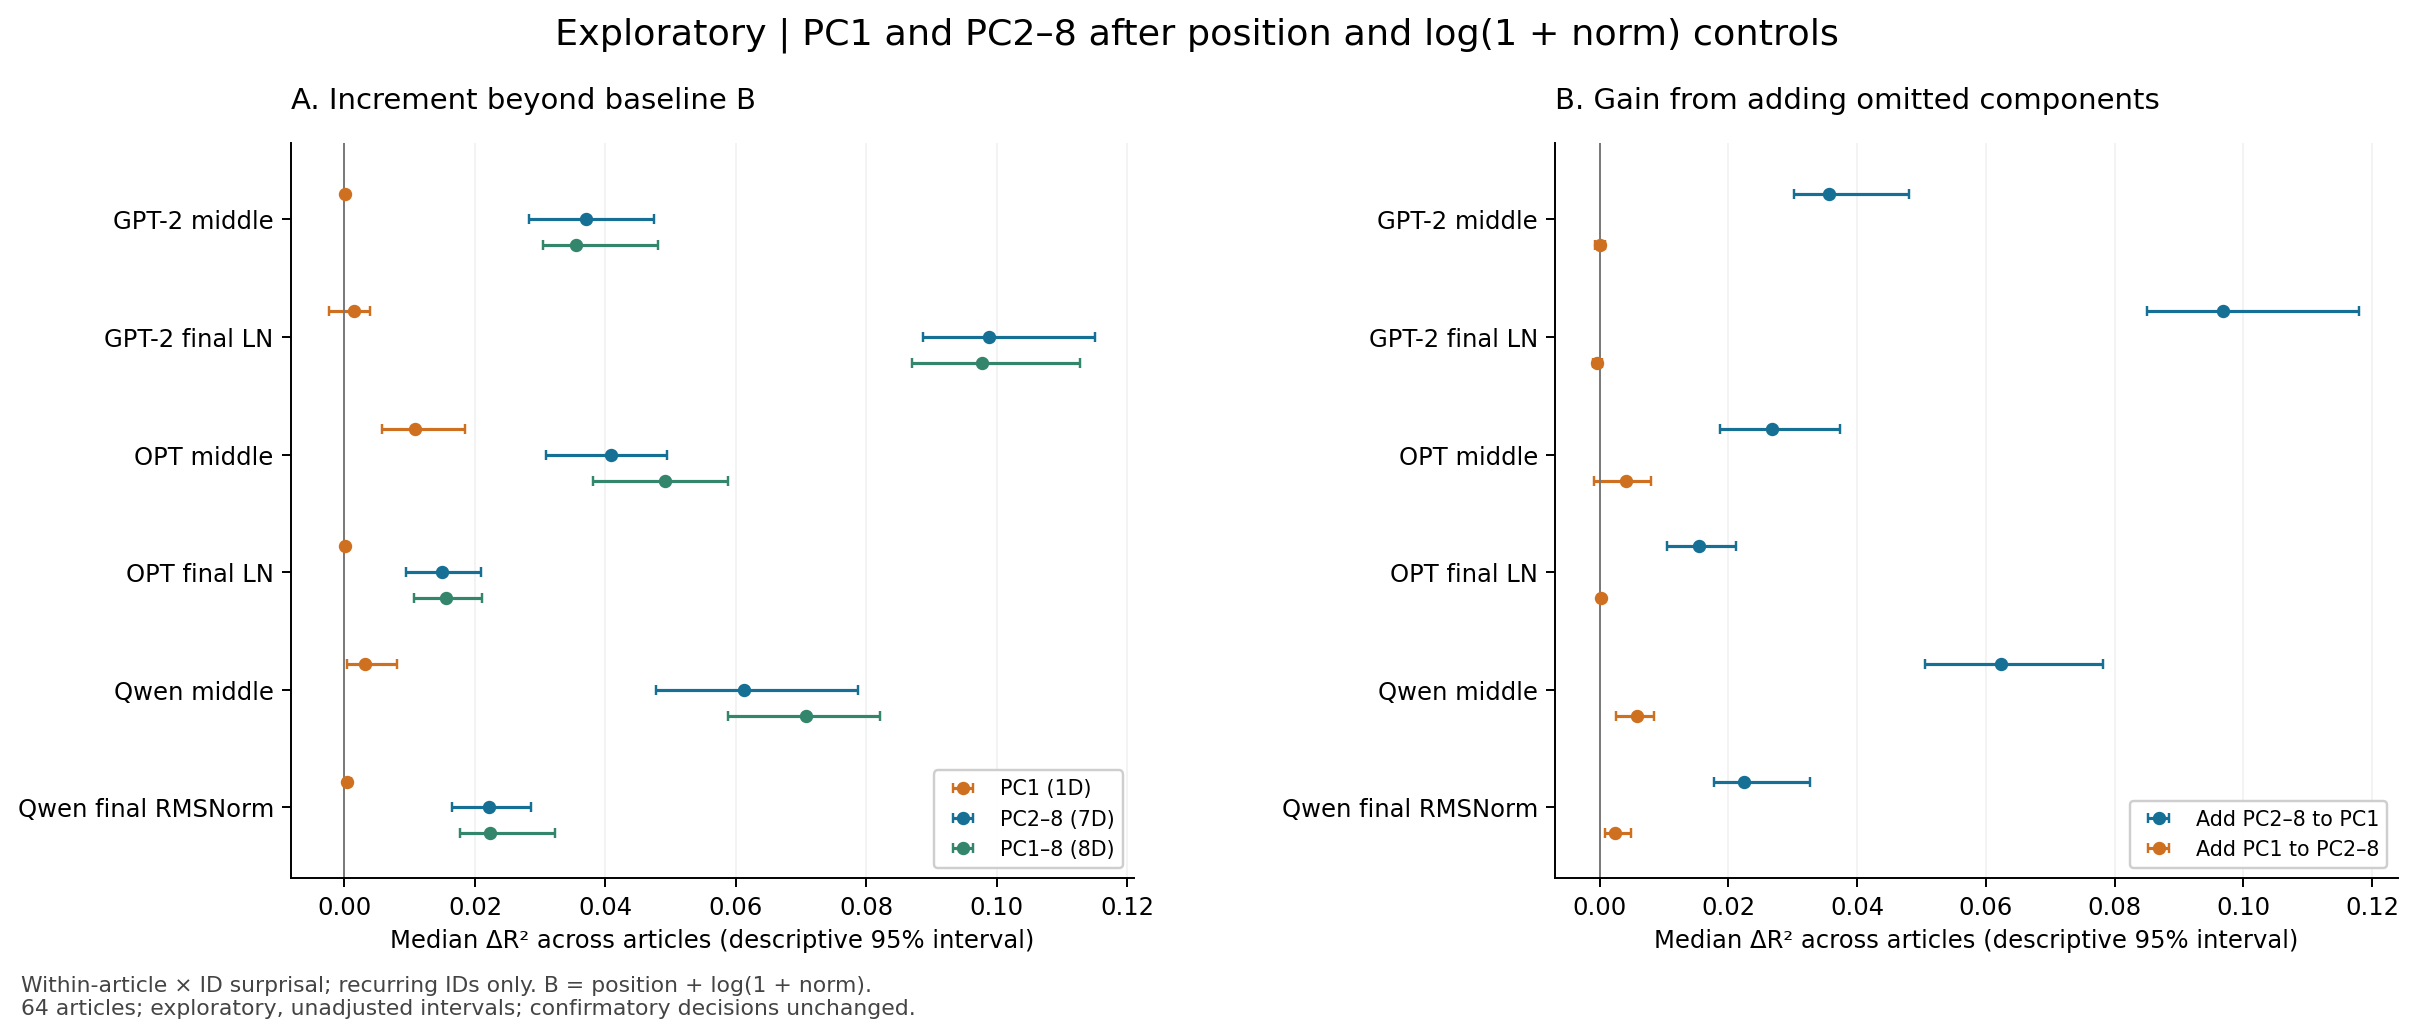
\includegraphics[width=\linewidth,height=0.74\textwidth,keepaspectratio]{figures/07_eda_components.png}
\captionof*{figure}{Figure 7. Exploratory within-article × ID surprisal readout on recurring IDs. The baseline B contains position terms and log1p hidden-state norm. Left: increments from PC subsets over B. Right: paired gains from adding the omitted components. Points and bars are medians across articles and unadjusted descriptive 95\% intervals.}
\end{landscape}

\FloatBarrier

\subsection{6.4 Direction supports readout after accounting for overlap with length}\label{direction-supports-readout-after-accounting-for-overlap-with-length}

PC scores depend on both the norm and direction of a hidden-state vector. We therefore compared the top eight PCs of raw states (raw PC1--8) with eight PCs fitted to unit-length states (U8), after adding a flexible norm control to the baseline. Writing \(r=\|h\|\) and \(u=h/r\), this control, N, adds five hinge functions of log(1 + r). U8 and its random controls both project the same centered unit-length states. Appendix A.6 specifies the knots, standardization, and regression.

Even after flexible modeling of length, the increment from U8 was positive in every condition examined. Its advantage over random directions was near zero at OPT's middle layer, while the other conditions had positive descriptive intervals (Table 12). Direction-related features therefore supported additional readout after the specified length associations were included in the baseline.

\Needspace{6\baselineskip}\begingroup
\fontsize{9.3}{12}\selectfont\setlength{\tabcolsep}{3.3pt}
{
\begin{longtable}[]{@{}
  >{\raggedright\arraybackslash}p{(\linewidth - 6\tabcolsep) * \real{0.2000}}
  >{\raggedleft\arraybackslash}p{(\linewidth - 6\tabcolsep) * \real{0.1800}}
  >{\raggedright\arraybackslash}p{(\linewidth - 6\tabcolsep) * \real{0.3000}}
  >{\raggedright\arraybackslash}p{(\linewidth - 6\tabcolsep) * \real{0.3200}}@{}}
\caption*{\textbf{Table 12. Exploratory readout beyond the flexible length control N.} Medians across 64 articles. U8 columns include descriptive 95\% intervals.}\\
\toprule\noalign{}
\begin{minipage}[b]{\linewidth}\raggedright
Condition
\end{minipage} & \begin{minipage}[b]{\linewidth}\raggedleft
Raw PC1--8 increment over N
\end{minipage} & \begin{minipage}[b]{\linewidth}\raggedright
U8 increment over N {[}95\% interval{]}
\end{minipage} & \begin{minipage}[b]{\linewidth}\raggedright
U8 advantage over random directions {[}95\% interval{]}
\end{minipage} \\
\midrule\noalign{}
\endfirsthead
\caption*{\textbf{Table 12 (continued).}}\\
\toprule\noalign{}
\begin{minipage}[b]{\linewidth}\raggedright
Condition
\end{minipage} & \begin{minipage}[b]{\linewidth}\raggedleft
Raw PC1--8 increment over N
\end{minipage} & \begin{minipage}[b]{\linewidth}\raggedright
U8 increment over N {[}95\% interval{]}
\end{minipage} & \begin{minipage}[b]{\linewidth}\raggedright
U8 advantage over random directions {[}95\% interval{]}
\end{minipage} \\
\midrule\noalign{}
\endhead
\bottomrule\noalign{}
\endlastfoot
GPT-2 middle & 0.03313 & 0.04254 {[}0.03149, 0.05527{]} & 0.02341 {[}0.01259, 0.03215{]} \\*
GPT-2 final & 0.07778 & 0.08748 {[}0.08083, 0.09674{]} & 0.01858 {[}0.01654, 0.02721{]} \\*
OPT middle & 0.03055 & 0.01386 {[}0.00734, 0.01783{]} & 0.00016 {[}−0.00650, 0.00379{]} \\*
OPT final & 0.01383 & 0.01402 {[}0.01061, 0.01973{]} & 0.00726 {[}0.00435, 0.01384{]} \\*
Qwen middle & 0.07180 & 0.06761 {[}0.05332, 0.07637{]} & 0.04139 {[}0.02722, 0.04626{]} \\*
Qwen final & 0.02452 & 0.02082 {[}0.01581, 0.02611{]} & 0.01093 {[}0.00738, 0.02030{]} \\*
\end{longtable}
}
\endgroup

Strengthening the length control reduced the raw-PC increment particularly at GPT-2's final layer and OPT's middle layer. In these conditions, some associations readable from raw PCs overlapped with nonlinear associations involving length. Changes in the other conditions were small or positive, indicating that the degree of overlap also varied across models and layers (Figure 8, Table B3).

\clearpage\begin{landscape}\thispagestyle{plain}
\centering
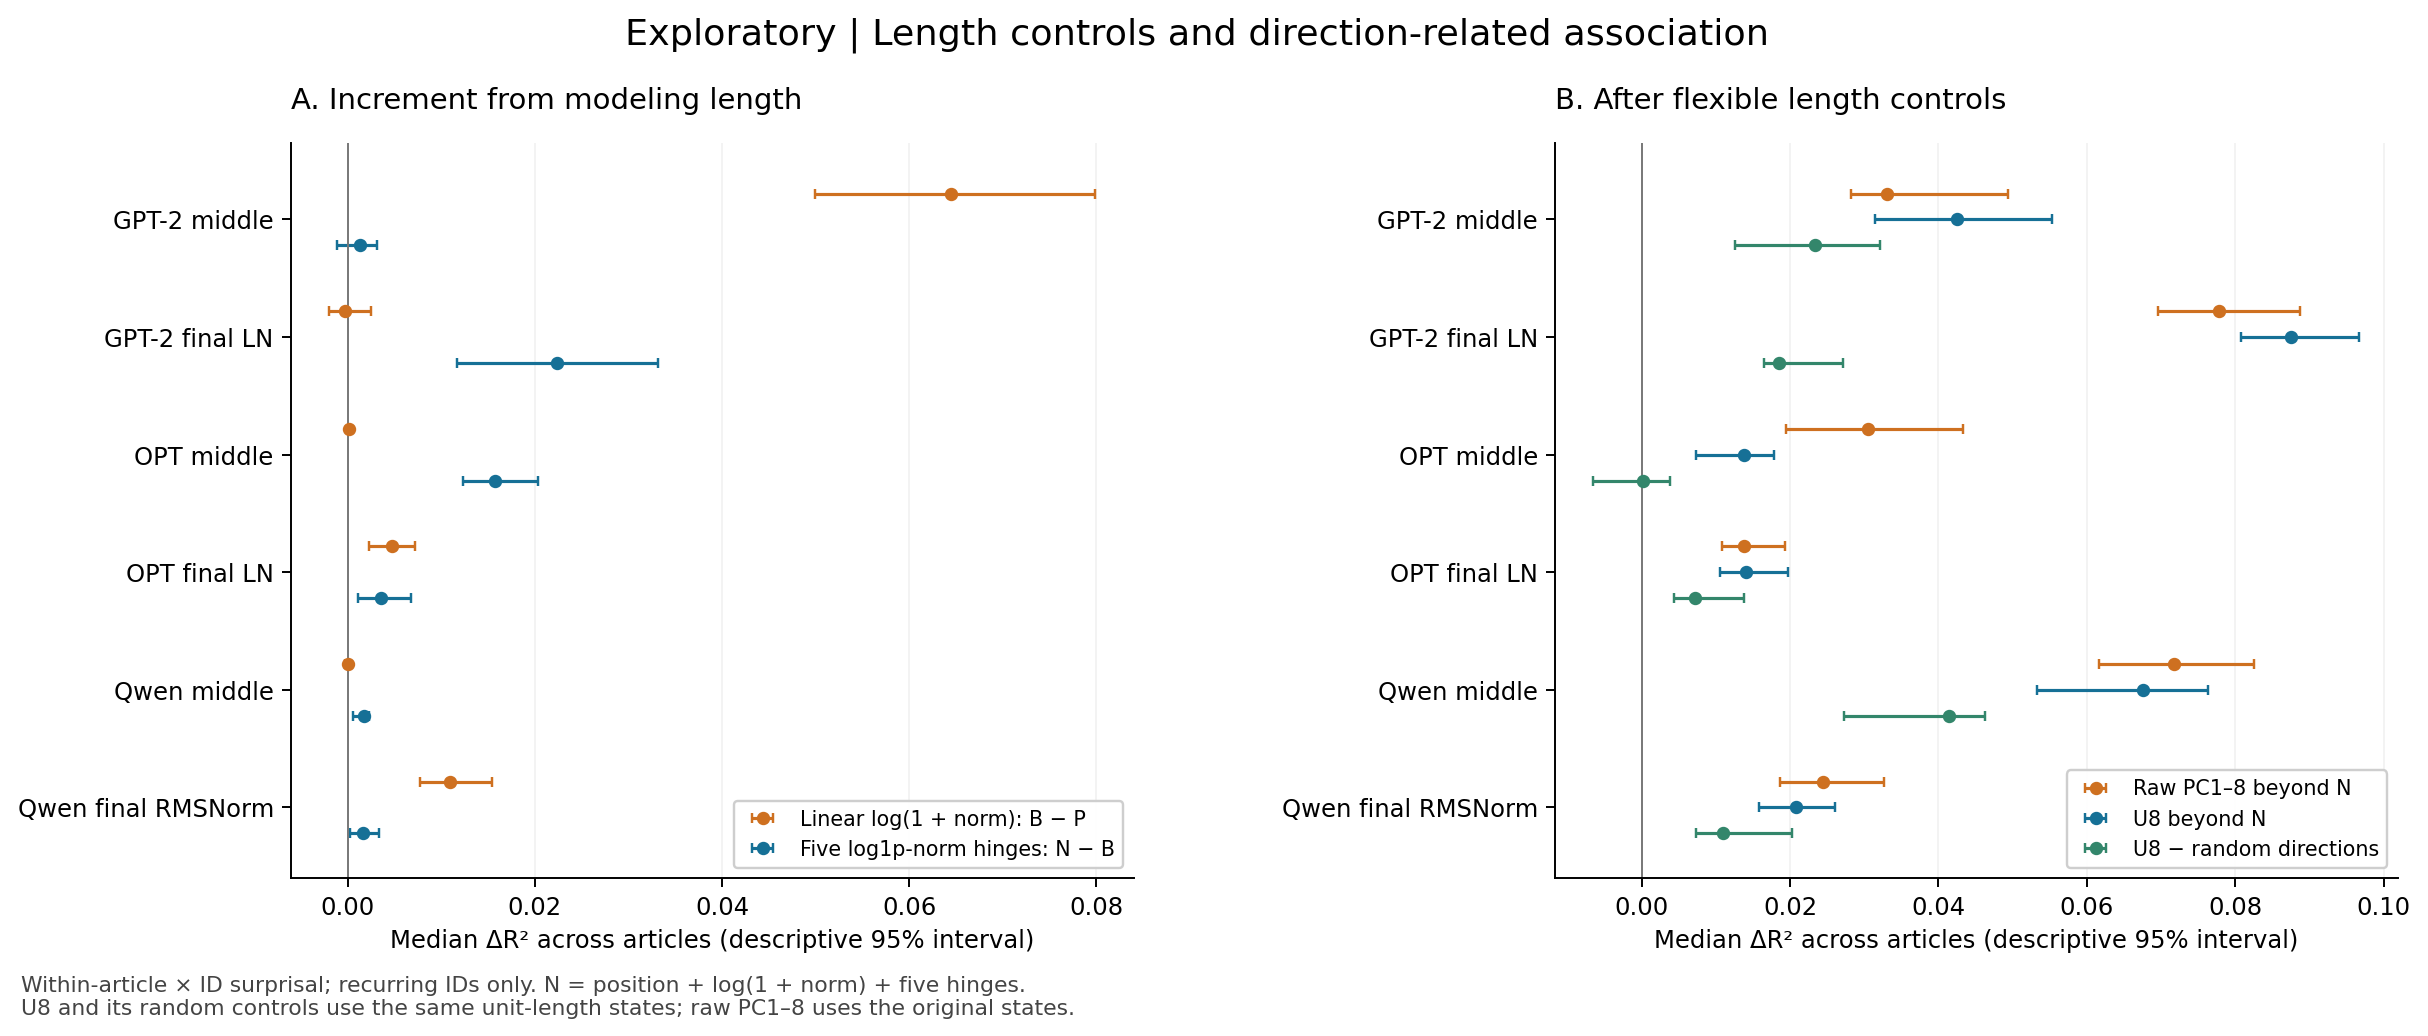
\includegraphics[width=\linewidth,height=0.74\textwidth,keepaspectratio]{figures/08_eda_radius_direction.png}
\captionof*{figure}{Figure 8. Exploratory within-article × ID surprisal readout on recurring IDs. Left: gains from adding log1p norm to the position-only baseline P (giving B), then 5 hinges of log1p norm (giving N). Right: increments over N from raw PC1--8 and unit-state PCs U8, and U8's advantage over random directions applied to the same unit states. Points and bars are medians across articles and unadjusted descriptive 95\% intervals.}
\end{landscape}

\FloatBarrier

\subsection{6.5 Typical improvements coexist with large losses concentrated in a few articles}\label{typical-improvements-coexist-with-large-losses-concentrated-in-a-few-articles}

We then examined how aggregate improvements related to imbalances across articles and tokens. Reweighting evaluation to give recurring IDs equal weight left positive median increments for raw PCs and U8 in every condition. At Qwen's middle layer, however, improvement on many articles coexisted with a large deterioration on one article.

Adding raw PCs produced a large readout failure on \nolinkurl{wt2_train_27981} (2nd Battalion 9th Marines), making the mean article-level increment negative despite a positive median. Its {\(\Delta\)R\textsuperscript{2}} of about −24 means that the augmented model's SSE exceeded the baseline SSE by about 24 times that article's within-group target sum of squares. The loss was smaller with N + U8 (Table 13, Figure 9). The two columns differ in both baseline and representation; using the same baseline N yielded increments of −30.578826 for raw PC1--8 and −0.265742 for U8 on this article. Table B3 gives intervals and absolute performance.

\Needspace{6\baselineskip}\begingroup
\fontsize{9.3}{12}\selectfont\setlength{\tabcolsep}{3.3pt}
{
\begin{longtable}[]{@{}
  >{\raggedright\arraybackslash}p{(\linewidth - 4\tabcolsep) * \real{0.3900}}
  >{\raggedleft\arraybackslash}p{(\linewidth - 4\tabcolsep) * \real{0.3200}}
  >{\raggedleft\arraybackslash}p{(\linewidth - 4\tabcolsep) * \real{0.2900}}@{}}
\caption*{\textbf{Table 13. Aggregate quantities and the failure article at Qwen's middle layer.} Exploratory description retaining all 64 articles. Both the baseline and the added representation differ between columns.}\\
\toprule\noalign{}
\begin{minipage}[b]{\linewidth}\raggedright
Quantity
\end{minipage} & \begin{minipage}[b]{\linewidth}\raggedleft
Raw PC1--8 / position-and-log1p-norm baseline
\end{minipage} & \begin{minipage}[b]{\linewidth}\raggedleft
U8 / flexible length baseline N
\end{minipage} \\
\midrule\noalign{}
\endfirsthead
\caption*{\textbf{Table 13 (continued).}}\\
\toprule\noalign{}
\begin{minipage}[b]{\linewidth}\raggedright
Quantity
\end{minipage} & \begin{minipage}[b]{\linewidth}\raggedleft
Raw PC1--8 / position-and-log1p-norm baseline
\end{minipage} & \begin{minipage}[b]{\linewidth}\raggedleft
U8 / flexible length baseline N
\end{minipage} \\
\midrule\noalign{}
\endhead
\bottomrule\noalign{}
\endlastfoot
Median article-level increment & 0.07077 & 0.06761 \\*
Mean article-level increment & −0.31019 & 0.06005 \\*
Increment on the failure article above & −24.22476 & −0.26574 \\*
\end{longtable}
}
\endgroup

The failure persisted when the fixed predictions were reconstructed through a separate computational route and when recurring IDs received equal scoring weight. We also summed token-level squared-error improvements, divided by each article's target sum of squares, within categories. Negative mean contributions were large for tokens containing letters, low-frequency tokens, and the opening portion of articles. These additive totals describe where losses accumulated; category counts and exposure differ. Appendix A.6 defines the categories, and \href{../references/tables/appendix_J.md}{Detailed Table Set J} reports all contributions, token shares, and article counts.

This diagnostic captures both the gain for a typical article and the influence of articles where losses are concentrated. Assessing the readout value of PCs requires considering representative performance alongside its distribution across articles.

\clearpage\begin{landscape}\thispagestyle{plain}
\centering
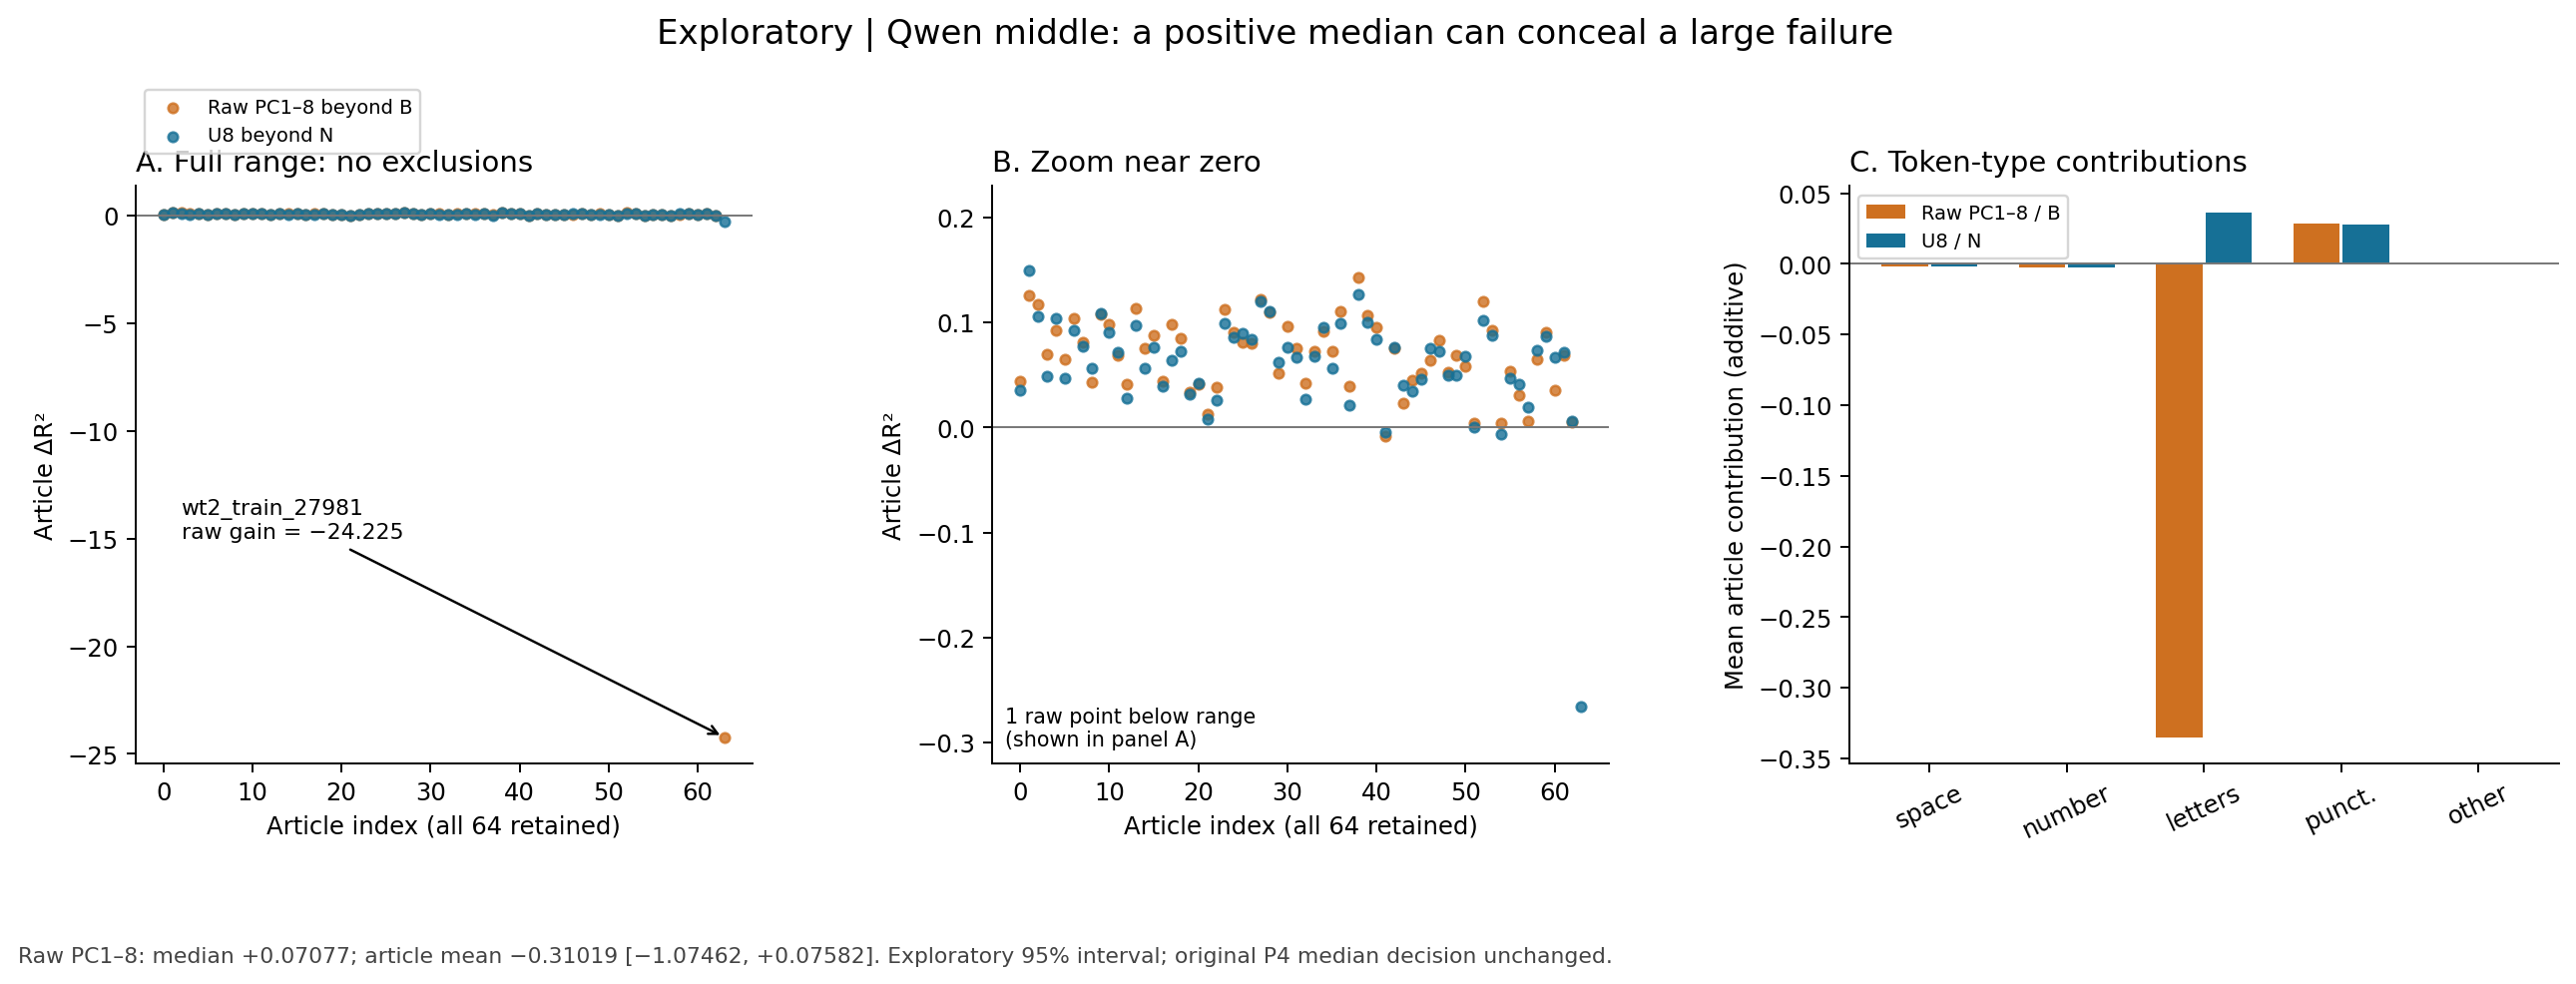
\includegraphics[width=\linewidth,height=0.74\textwidth,keepaspectratio]{figures/09_eda_article_bias.png}
\captionof*{figure}{Figure 9. All 64 articles at Qwen's middle layer, comparing B + raw PC1--8 with N + U8 in within-article × ID surprisal evaluation. Both baseline and added representation differ. Left: full range. Center: magnification near zero; the raw-PC1--8 point outside this range is retained in the left panel. Right: additive mean contributions by token type, showing where error improvements and losses accumulate.}
\end{landscape}

\FloatBarrier

\subsection{6.6 Geometry and residual features also combine differently across article conditions}\label{geometry-and-residual-features-also-combine-differently-across-article-conditions}

We explored the relationship between article point distributions and residual features using saved P4 states (EDA-0004). All 1,152 article conditions were retained, covering every model, extraction point, and C0/C1/C4 treatment. After defining measurements in this exploration, we planned the short-text geometry study reported in Section 3.

At the middle layers of GPT-2 and Qwen, the all-point long axis arose from a distant, highly influential point and a dense cloud. Concentration at OPT's middle layer was weaker. After GPT-2's final normalization, by contrast, the points formed an elongated band with appreciable width and curvature (Figure 10). Fit quality in a projected plane differed from the extent to which a single curve approximated the full hidden state, as did the number of articles meeting the criteria (Table 14). Table C2 reports all 18 conditions, including the sensitivity treatments.

\Needspace{6\baselineskip}\begingroup
\fontsize{9.3}{12}\selectfont\setlength{\tabcolsep}{3.3pt}
{
\begin{longtable}[]{@{}
  >{\raggedright\arraybackslash}p{(\linewidth - 10\tabcolsep) * \real{0.2900}}
  >{\raggedleft\arraybackslash}p{(\linewidth - 10\tabcolsep) * \real{0.1400}}
  >{\raggedleft\arraybackslash}p{(\linewidth - 10\tabcolsep) * \real{0.1600}}
  >{\raggedleft\arraybackslash}p{(\linewidth - 10\tabcolsep) * \real{0.1500}}
  >{\raggedleft\arraybackslash}p{(\linewidth - 10\tabcolsep) * \real{0.1100}}
  >{\raggedleft\arraybackslash}p{(\linewidth - 10\tabcolsep) * \real{0.1500}}@{}}
\caption*{\textbf{Table 14. Exploratory geometry measurements on saved articles.} C0; 64 articles per condition. Q is the article median. ``2D distribution criterion'' is the joint occupancy, gap, single-point contribution, and curve-Q criterion; ``also curved'' counts those additionally meeting the improvement-over-line criterion. The full-space column evaluates Q on the complete state.}\\
\toprule\noalign{}
\begin{minipage}[b]{\linewidth}\raggedright
Model and extraction point (C0)
\end{minipage} & \begin{minipage}[b]{\linewidth}\raggedleft
Curve Q: 2D
\end{minipage} & \begin{minipage}[b]{\linewidth}\raggedleft
Curve Q: full space
\end{minipage} & \begin{minipage}[b]{\linewidth}\raggedleft
2D distribution criterion
\end{minipage} & \begin{minipage}[b]{\linewidth}\raggedleft
Also curved
\end{minipage} & \begin{minipage}[b]{\linewidth}\raggedleft
Full-space distribution criterion
\end{minipage} \\
\midrule\noalign{}
\endfirsthead
\caption*{\textbf{Table 14 (continued).}}\\
\toprule\noalign{}
\begin{minipage}[b]{\linewidth}\raggedright
Model and extraction point (C0)
\end{minipage} & \begin{minipage}[b]{\linewidth}\raggedleft
Curve Q: 2D
\end{minipage} & \begin{minipage}[b]{\linewidth}\raggedleft
Curve Q: full space
\end{minipage} & \begin{minipage}[b]{\linewidth}\raggedleft
2D distribution criterion
\end{minipage} & \begin{minipage}[b]{\linewidth}\raggedleft
Also curved
\end{minipage} & \begin{minipage}[b]{\linewidth}\raggedleft
Full-space distribution criterion
\end{minipage} \\
\midrule\noalign{}
\endhead
\bottomrule\noalign{}
\endlastfoot
GPT-2 middle & -796.1 & -2.803e+04 & 0/64 & 0/64 & 0/64 \\*
GPT-2 after final normalization & 0.9282 & 0.8605 & 39/64 & 19/64 & 5/64 \\*
OPT middle & 0.48 & -0.3569 & 0/64 & 0/64 & 0/64 \\*
OPT after final normalization & 0.5365 & 0.03684 & 0/64 & 0/64 & 0/64 \\*
Qwen middle & -1.105e+07 & -1.49e+08 & 0/64 & 0/64 & 0/64 \\*
Qwen after final normalization & 0.7039 & 0.2451 & 0/64 & 0/64 & 0/64 \\*
\end{longtable}
}
\endgroup

\begin{figure}[!htbp]
\centering
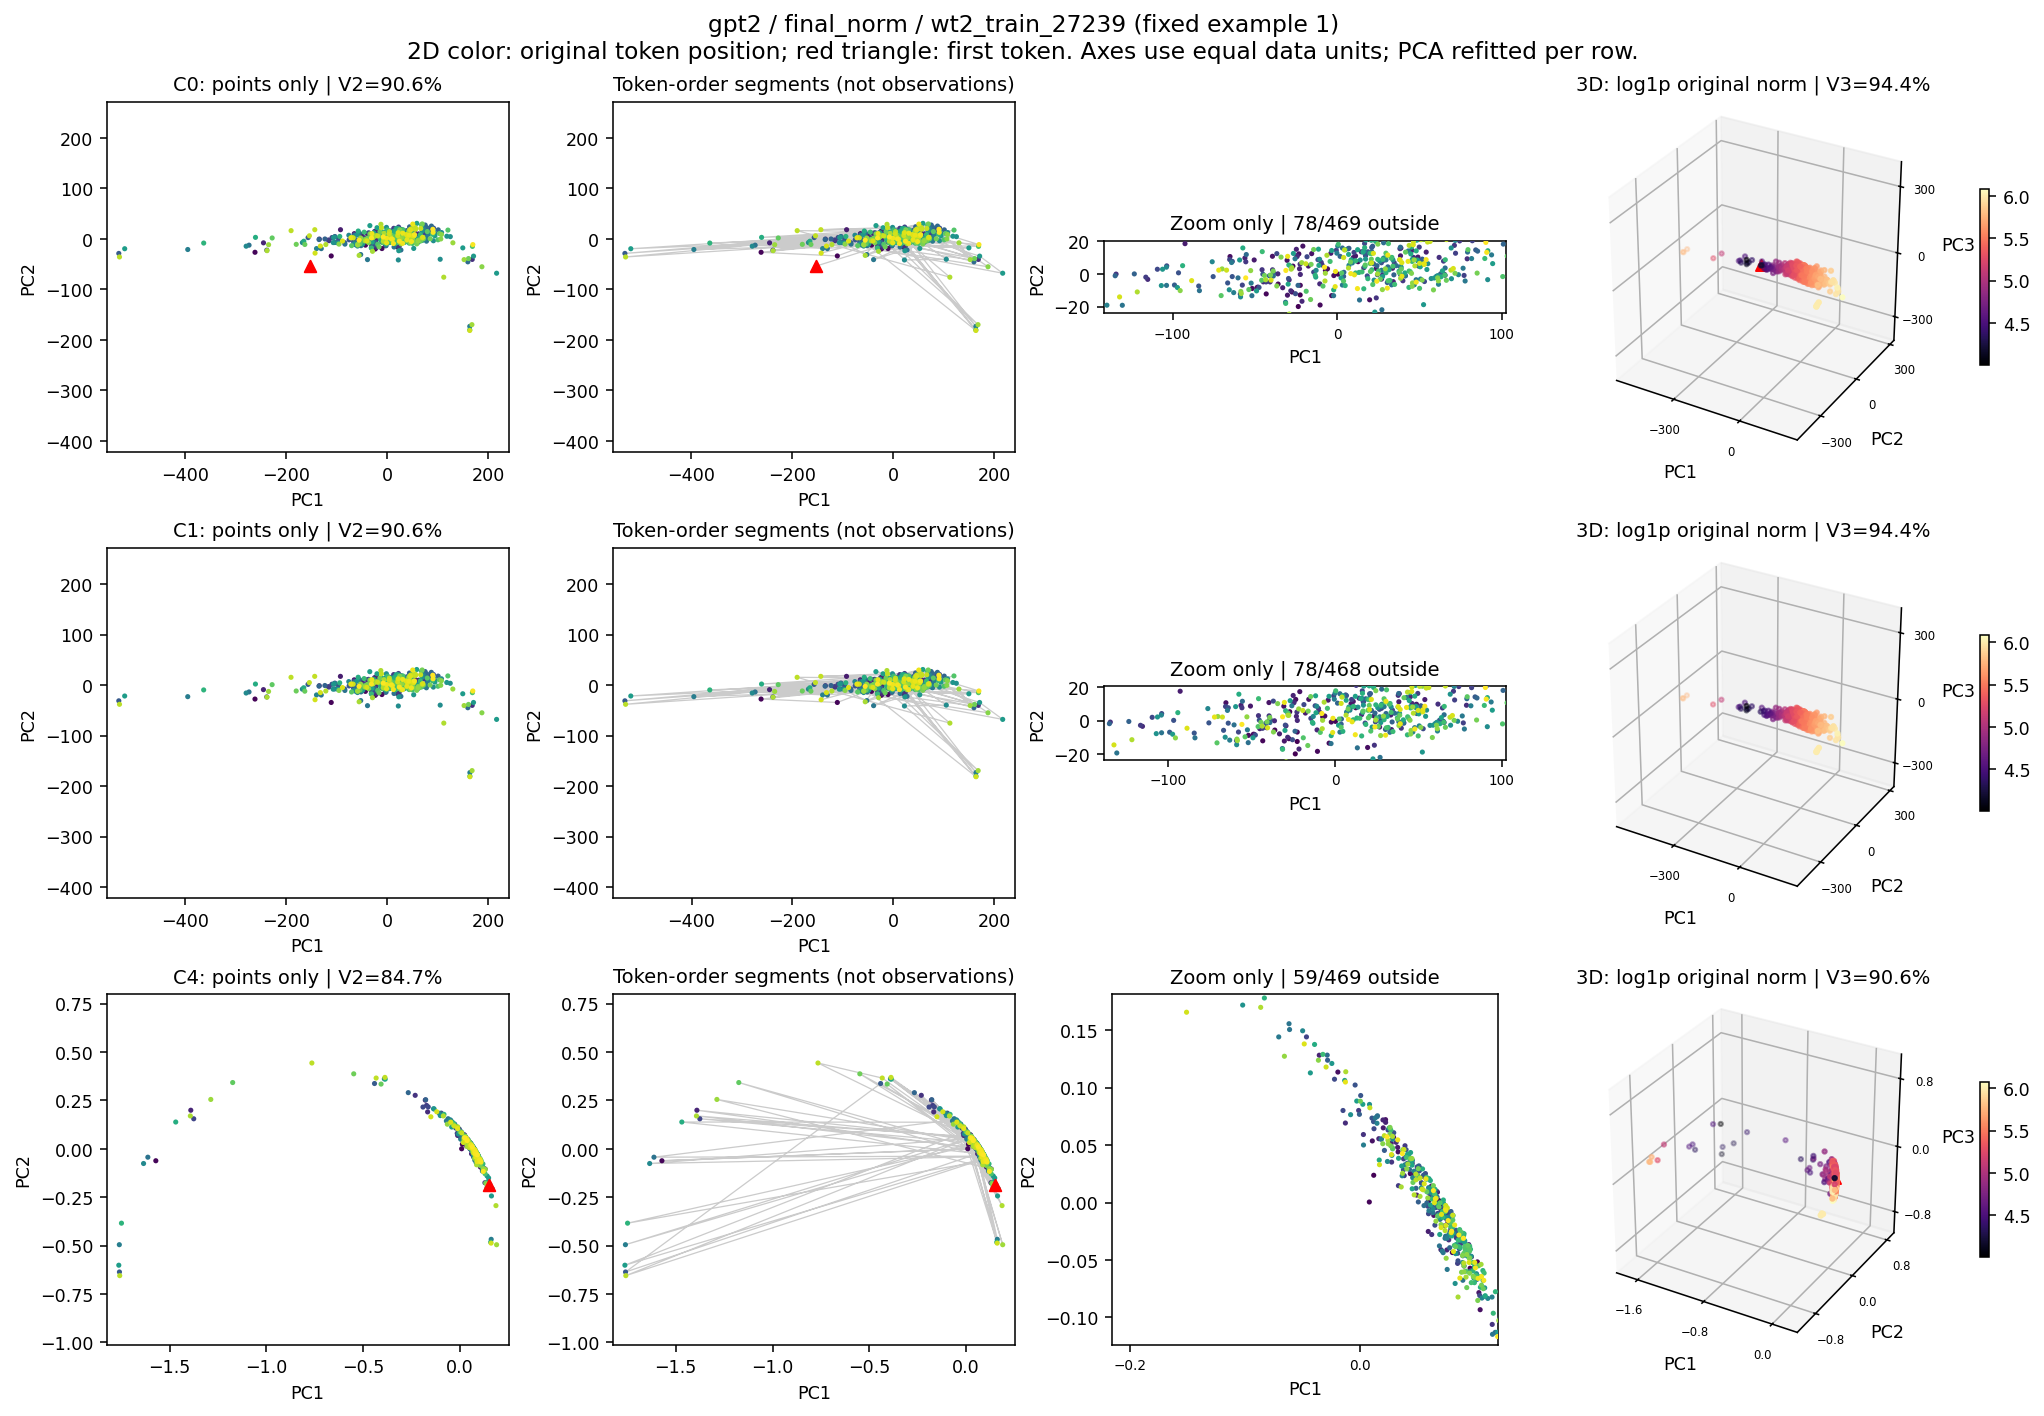
\includegraphics[width=\linewidth,height=0.73\textheight,keepaspectratio]{figures/10_article_shape.png}
\captionof*{figure}{Figure 10. GPT-2 after final normalization for example article wt2\_train\_27239, selected by an ID hash before analysis. V2/V3 denote cumulative variance ratios for the top 2/3 components. Compare C0 with C1 in the left column first, then C4 and the magnified column. Token-order lines and 3D views provide supplementary displays; 3D color denotes log1p original norm. Points outside the magnified range remain in every analysis. Tables 14 and C2 summarize all 64 articles.}
\end{figure}

Adding the seven local residual coordinates to the controlled surprisal readout produced positive descriptive intervals for the median increment in all 18 conditions (Appendix C.4). These are within-article readouts conditional on full-article coordinates: PCA and quadratic residualization use all included states, while the readout fit holds out each block's target labels. At Qwen's middle layer, one article incurred an enormous loss concentrated at a distant high-norm state, making the article mean strongly negative (Table C3). That state was at position 1 and remained after position 0 was excluded. Appendix C.4 gives its norm and the training-fold range, documenting the out-of-range observation associated with the error.

The local analysis describes which features accompany variation around each article's main axis. The shared-basis analysis in Section 4 tests whether coordinates and readouts fitted on training articles remain useful on other articles. Together, they describe residual variation and transferable readout while preserving the distinction between the two coordinate constructions.

\FloatBarrier

\section{7. General discussion}\label{general-discussion}

The results yield three empirical lessons for interpreting PCA visualizations and probes. First, a dominant PC can reflect a small number of influential observations. At GPT-2's middle layer, the distant first-token state accounts for much of the apparent long axis; the remaining points occupy a far less concentrated cloud. Point distributions, gaps, and PCA refitted after first-token exclusion explain what the high variance ratio summarizes.

Second, reducing this concentration leaves useful variation. Shared PCs support incremental current-token surprisal readout after the specified lexical controls, including deviations among occurrences of the same ID within an article. The PC-versus-random ranking changes with the training configuration, so the result must be interpreted together with the population, objective, and penalties used to fit the readout.

Third, a positive median gain describes the typical article without establishing stability across the sample. At Qwen's middle layer, one severe failure makes the article mean negative. Showing the full distribution reveals a property that the median alone misses.

These findings link the appearance of variance concentration to controlled readout and its distribution across articles. The local geometry and shared-basis experiments address different constructions; directly relating their subspaces remains an open question. The present results establish what each construction reveals and where its readout becomes unreliable.

\FloatBarrier

\section{8. Limitations and unresolved questions}\label{limitations-and-unresolved-questions}

This section consolidates the qualifications relevant to interpreting and generalizing the results.

\FloatBarrier

\subsection{8.1 Readable associations and causal mechanisms}\label{readable-associations-and-causal-mechanisms}

We measured associations that can be statistically read from hidden states. The results do not establish that a model causally uses those directions, that particular PCs constitute necessary circuits, or that PC2--8 are independent semantic factors. Orthogonality in PCA does not guarantee independence of linguistic functions.

The surprisal target is determined from logits before the current token is read, whereas the explanatory state is obtained after that token is processed. Performance therefore does not measure the ability to predict an unseen next token or an improvement in the language model itself. Centering targets and predictions within groups for evaluation likewise does not imply that the group mean of unknown labels can be predicted in deployment.

\FloatBarrier

\subsection{8.2 Scope of the controls and decompositions}\label{scope-of-the-controls-and-decompositions}

Within-ID comparisons remove mean differences specific to each ID, but do not remove every effect of position, context content, or uncontrolled nonlinear relationships. The NL model in EDA-0001 was weaker than the ID model, and the strongest conceivable lexical and nonlinear controls have not been exhausted. The roughly halved PC increment cannot be interpreted as showing that half of the effect is causally attributable to lexical identity.

PC subsets involve re-estimating penalties and coefficients, so their increments are not an additive decomposition of contributions. A small incremental value for PC1 is conditional on already accounting for position and norm; it does not imply that PC1 is uninformative in absolute terms.

Raw-state PC1--8 and unit-state U8 use different bases. Raw-state projections include a length-by-direction product, whereas N + U8 is an additive readout. Their performance difference cannot be converted into a pure contribution of length or an effect of information loss from normalization. An association beyond a finite control with 5 hinges also cannot be declared independent of every possible length association. Random controls match dimensionality and tuning opportunities, but not captured variance. An advantage over them is not evidence of semantic specificity.

\FloatBarrier

\subsection{8.3 Statistical uncertainty and exploration}\label{statistical-uncertainty-and-exploration}

Confirmatory adjustments were made within each stage. They do not jointly adjust for sequential hypothesis formation and model selection throughout the study. The local preregistrations have no public registry or third-party timestamp certification. Bootstrap intervals are finite-sample approximations and describe variation across articles conditional on the frozen training basis, coefficients, and controls.

Internal cross-validation from P2 onward includes conditional tuning that shares PCA bases or scales estimated from the full training set. It is not a fully nested cross-validation estimate of generalization performance. The intervals also exclude variation from resampling the training sample or choosing different model weights.

Evaluation articles in the additional analyses were already known, and the 95\% intervals are exploratory descriptions without adjustment for multiple comparisons. They do not change P4's 4 supported and 2 inconclusive outcomes into 6 supported outcomes. Inconclusive does not mean absence of an effect or experimental failure. Support in one condition and an inconclusive outcome in another also do not establish a difference between conditions or a model-by-layer interaction. Table 8 assesses criterion attainment separately by condition; it does not test a ranking of models. Changes across O/R/W involve the training population, objective, and penalties, so the full change cannot be attributed to a single factor.

\FloatBarrier

\subsection{8.4 Coverage and article-level failures}\label{coverage-and-article-level-failures}

The study covers selected models, English WikiText-2 passages of restricted length, and three fixed English short texts. The 3 models in P4 were purposively selected. Generalization to all LLMs, other languages, domains, or long documents remains untested. Articles unused in this study are not guaranteed to have been unseen during the language models' pretraining.

The P4 models also differ in tokenizer, their own surprisal targets, training data, size, and positional representations. Their comparison does not isolate a causal effect of LayerNorm versus RMSNorm. The common input setting without an added BOS token can also differ from model-recommended formats. Within-ID evaluation is restricted to recurring IDs and does not directly support conclusions about IDs occurring only once.

The large failure at Qwen's middle layer shows that favorable median performance does not guarantee favorable mean performance or stability on every article. Although the failure was smaller with N + U8, the directional basis, coefficients, and functional form also changed. This observation does not isolate normalization as the cause or identify norm anomalies, particular words, or extrapolation as the causal explanation. The original failure article was retained without exclusion, repair, or reselection of conditions.

\FloatBarrier

\subsection{8.5 Scope of geometric measurements and mechanisms that produce the geometry}\label{scope-of-geometric-measurements-and-mechanisms-that-produce-the-geometry}

Excluding the first token from an analysis of saved states is not an intervention that removes the token from the input and reruns the model. The circuitry producing the large first-token state and the reason concentration persists after final normalization remain unidentified.

The three texts in the short-text geometry study were known at design time and are not counted as a sample confirming generalization to unknown articles. The results apply to the chosen weight revision, dependency versions, attention implementation, and PCA via full SVD. A good curve fit in a short text provides limited grounds for claiming a shape common to arbitrary texts or all layers.

The operational arc criteria concern a quadratic graph parameterized by PC1 and the occupancy and gaps of sampled points. The thresholds are not tests calibrated under a noise model, and they do not exhaustively assess folds, multiple branches, higher-order curves, or true intrinsic dimensionality. We report failure to meet the criteria alongside good local or condition-dependent curve fits.

PCA in the geometry analysis uses all included points in an article, including held-out blocks. The block-held-out Q is therefore a descriptive diagnostic conditional on fixed coordinates, not predictive performance on unknown texts. Large negative Q values include extrapolation failures of the specified regression. Thickness, defined as seven residual coordinates, is not the shortest distance to a curve, and component indices within an article cannot be equated with indices in the shared basis. We have not directly tested the correspondence between local-residual and shared-PC subspaces, transfer of the same residual features to separate articles, or why local geometry might enable transfer. Nor have we separated geometric constraints associated with normalization from contributions of linguistic organization. These associations do not establish semantically dedicated axes or layers of discrete linguistic functions.

\FloatBarrier

\subsection{8.6 Verification scope and remaining questions}\label{verification-scope-and-remaining-questions}

Checks performed after the experiment outputs were received found agreement between saved results and calculations performed through separate computational routes. They were not independent replications using a separately implemented language-model forward pass. Generation and verification include self-audits by the same agent; independent replication by another researcher has not been performed.

The GPU used for the short-text check was an NVIDIA L4, differing from the candidate hardware in the execution plan. The primary CPU condition was retained, with inputs, weights, and numerical settings fixed. Of 12 CPU/GPU state pairs, 1 exceeded the fixed tolerance, although geometric decisions agreed for all 36 corresponding conditions. The excess occurred at 1 of 55,296 coordinates for the repetitive passage before final LayerNorm and was recorded without changing the tolerance (Table C4).

The main remaining questions concern (i) the computations producing first-token and final-layer concentration, (ii) the composition of associations readable within the same ID, (iii) the causal role of PC directions in the model's computations, and (iv) the conditions that produce large article-level losses. Resolving them requires evidence beyond the current readout comparisons.

\FloatBarrier

\section{9. Conclusion}\label{conclusion}

The first token strongly influences the prominent variance concentration at GPT-2's middle layer. After its exclusion from analysis, a training-fitted shared basis retains position correlations on separate articles, and shared-PC surprisal readouts show positive median increments beyond the specified lexical controls, including within recurring article × ID groups. The multi-model confirmation supports four of six conditions under within-group training. Exploratory diagnostics locate additional associations in PC2--8 and unit-state directions, while revealing sensitivity to training configuration and severe article-level failures. \textbf{Variance concentration, transferable readout, and stability across articles are distinct properties of Transformer representations.} Examining them together makes the interpretation of principal components more precise.

\FloatBarrier

\section{Data, code, and verification records}\label{data-code-and-verification-records}

Appendices A--C contain the main methods and supplementary results needed to assess the claims. Tables covering all conditions, articles, and random sets, along with original ZIP archives, fixed predictions, coefficients, inputs, code, and verification records, are accessible through the \href{../references/README.md}{reference-materials guide}. The \href{../references/FIGURE_TABLE_MAP.md}{figure and table map} links each result to its corresponding summaries and data. This version is for local distribution; a public repository and external download URLs have not yet been assigned. The \href{../references/MANIFEST.json}{SHA-256 manifest} identifies the manuscript, figures, and fixed reference materials.

\FloatBarrier

\section{Authorship and assistance}\label{authorship-and-assistance}

The author ran the experiments in Colab. An LLM agent assisted with design, code development, verification after receipt, analysis, and writing. Section 8.6 specifies the scope of verification.

\FloatBarrier

\section{References}\label{references}

{[}1{]} Kawin Ethayarajh. 2019. \emph{How Contextual are Contextualized Word Representations? Comparing the Geometry of BERT, ELMo, and GPT-2 Embeddings.} EMNLP-IJCNLP, 55--65. \href{https://aclanthology.org/D19-1006/}{Paper}

{[}2{]} Ziyang Luo, Artur Kulmizev, and Xiaoxi Mao. 2021. \emph{Positional Artefacts Propagate Through Masked Language Model Embeddings.} ACL-IJCNLP, 5312--5327. \href{https://aclanthology.org/2021.acl-long.413/}{Paper}

{[}3{]} Mingjie Sun, Xinlei Chen, J. Zico Kolter, and Zhuang Liu. 2024. \emph{Massive Activations in Large Language Models.} arXiv:2402.17762. \href{https://arxiv.org/html/2402.17762v2}{Paper, v2}

{[}4{]} Alex Ning, Vainateya Rangaraju, and Yen-Ling Kuo. 2025. \emph{Visualizing LLM Latent Space Geometry Through Dimensionality Reduction.} arXiv:2511.21594, v1. \href{https://arxiv.org/html/2511.21594v1}{Paper, v1}

{[}5{]} Guillaume Alain and Yoshua Bengio. 2016. \emph{Understanding intermediate layers using linear classifier probes.} arXiv:1610.01644. \href{https://arxiv.org/abs/1610.01644}{Paper}

{[}6{]} John Hewitt and Percy Liang. 2019. \emph{Designing and Interpreting Probes with Control Tasks.} EMNLP-IJCNLP. \href{https://aclanthology.org/D19-1275/}{Paper}

{[}7{]} Stephen Merity, Caiming Xiong, James Bradbury, and Richard Socher. 2016. \emph{Pointer Sentinel Mixture Models.} arXiv:1609.07843. \href{https://arxiv.org/abs/1609.07843}{Paper}



\FloatBarrier

\clearpage

\section{Appendix A. Core methods and decision rules}\label{appendix-a.-core-methods-and-decision-rules}

\FloatBarrier

\subsection{A.1 Inputs, extraction points, and numerical settings}\label{a.1-inputs-extraction-points-and-numerical-settings}

The article experiments used the original train split of Salesforce/wikitext, configuration \nolinkurl{wikitext-2-raw-v1}. An ``article'' is a document unit formed by splitting Parquet text rows at headings enclosed by single \nolinkurl{=} signs. Row indices are zero-based. Headings and body rows beginning with \nolinkurl{=} were excluded; nonempty rows were stripped and joined with two newlines. Titles were casefolded and whitespace sequences collapsed to a single space. We tokenized the first 8192 Unicode characters of each candidate body. P1--P3 used the first 512 tokens of candidates with at least 512 tokens. For duplicate normalized titles or identical leading token sequences, only the first occurrence was retained.

We rehashed each body SHA-256 with a stage-specific prefix and selected candidates in ascending hash order, breaking ties by article ID. P1 used 64 articles. P2 excluded P1 and selected 64 training and 64 evaluation articles; P3 excluded P1/P2 and selected 64 new evaluation articles; P4 excluded the 256 previously used articles and selected 64 new training and 64 new evaluation articles. From P2 onward, we also excluded token-prefix matches to preparatory short texts and near duplicates with GPT-2 token 5-gram set Jaccard similarity at least 0.5 to existing or already selected articles. Model outputs were not used for selection, and articles were not replaced after inspecting results.

P4 selected from 629 candidates. For each tokenizer, we identified the end of its 512th token, or its last token if fewer than 512, and used the earliest of these endpoints as a common upper bound. The same text string was cut at the preceding whitespace boundary. If retokenization exceeded 512 tokens, the text was shortened at whitespace boundaries. All models were required to receive 256--512 tokens. P5 used the three full texts in C.1, containing 101/85/72 tokens.

\Needspace{6\baselineskip}\begingroup
\fontsize{9.3}{12}\selectfont\setlength{\tabcolsep}{3.3pt}
{
\begin{longtable}[]{@{}
  >{\raggedright\arraybackslash}p{(\linewidth - 6\tabcolsep) * \real{0.2500}}
  >{\raggedright\arraybackslash}p{(\linewidth - 6\tabcolsep) * \real{0.3400}}
  >{\raggedleft\arraybackslash}p{(\linewidth - 6\tabcolsep) * \real{0.1000}}
  >{\raggedright\arraybackslash}p{(\linewidth - 6\tabcolsep) * \real{0.3100}}@{}}
\toprule\noalign{}
\begin{minipage}[b]{\linewidth}\raggedright
Model
\end{minipage} & \begin{minipage}[b]{\linewidth}\raggedright
Fixed weights and tokenizer revision
\end{minipage} & \begin{minipage}[b]{\linewidth}\raggedleft
Dimension
\end{minipage} & \begin{minipage}[b]{\linewidth}\raggedright
Middle / final article extraction point
\end{minipage} \\
\midrule\noalign{}
\endhead
\bottomrule\noalign{}
\endlastfoot
openai-community/gpt2 & \nolinkurl{607a30d783dfa663caf39e06633721c8d4cfcd7e} & 768 & After block 6 of 12 / after ln\_f \\*
facebook/opt-1.3b & \nolinkurl{3f5c25d0bc631cb57ac65913f76e22c2dfb61d62} & 2048 & After block 12 of 24 / after final\_layer\_norm \\*
Qwen/Qwen2.5-1.5B & \nolinkurl{8faed761d45a263340a0528343f099c05c9a4323} & 1536 & After block 14 of 28 / after final RMSNorm \\*
\end{longtable}
}
\endgroup

The corpus revision was \nolinkurl{b08601e04326c79dfdd32d625aee71d232d685c3} (CC-BY-SA-3.0 / GFDL). P1 collected GPT-2 states after blocks 1, 6, and 12 and after final LayerNorm; P2/P3 collected block 6 and the final normalized state. P5's primary condition was after block 7, with comparisons after blocks 6 and 12 and after final LayerNorm. Block numbering is one-based.

All models used eval mode, float32, eager attention, no quantization, TF32 disabled, and one text at a time. No BOS/EOS tokens, padding, or chat templates were added; the text began at position 0. P1--P4 used \nolinkurl{use_cache=False}; P5 used True. The reference environment was PyTorch 2.8.0+cu128, Transformers 4.57.6, and NumPy 2.2.6; post-acquisition analyses used float64. Input sets, exact extraction rules, seeds, and hashes are documented in the \href{../references/METHODS_AND_IDENTIFIERS.md}{methods and identifiers specification}.

\FloatBarrier

\subsection{A.2 PCA, preprocessing, and random controls}\label{a.2-pca-preprocessing-and-random-controls}

Let \(X_c\) be the state matrix \(X\) centered by the mean of included observations, and let \(\lambda_k\) be the eigenvalues of \(X_c^\top X_c/(n-1)\) in descending order. The PC1 variance ratio is \(V_1=\lambda_1/\sum_j\lambda_j\), the cumulative ratio of the top k components is \(\sum_{j\le k}\lambda_j/\sum_j\lambda_j\), and the norm association is \(R_1=|\operatorname{corr}(X_cu_1,\|h\|_2)|\). Signs are fixed by making the loading with the largest absolute value positive.

C0--C4 use the treatments in Section 2.3, retain original position indices, and re-estimate the mean and PCA for each condition. C2/C3 in P1 exclude 6 points; ties in norm rank follow original position order, and C3 averages 20 samples without replacement. P1/P5 used full SVD; the article-geometry exploration used Gram-matrix eigendecomposition. For P1 feature correlations, axes with eigenvalues {\(\leq\)} total variance × {10\textsuperscript{-}\textsuperscript{1}\textsuperscript{2}} were marked NA; correlations with post-treatment norm under C4 were also undefined.

The shared basis is estimated from one center and covariance matrix by concatenating included tokens from all 64 training articles with equal token weights. P2 estimates C0/C1/C4 separately; P3 reuses P2's C1 basis; P4 estimates a C1 basis. In P4, all C1 training tokens enter PCA and standardization, including tokens whose IDs occur only once in an article. O, R, and W share these estimates; their regression populations differ as specified in A.3. Evaluation articles use the training center and scales. P4 required the 8th eigenvalue \textgreater{} total variance × {10\textsuperscript{-}\textsuperscript{1}\textsuperscript{2}.} Eight was a fixed comparison dimensionality and was not optimized.

Random controls comprise 20 sets generated by reduced QR orthogonalization of standard normal matrices of hidden dimension \(D\times8\). PCG64 and fixed seeds were used, with the same sign convention, training-scale estimation, and tuning opportunities as for PCs. Errors were computed separately for each of the 20 sets within each article and then averaged; the best set was not selected. Component-subset comparisons use the corresponding first direction and remaining 7 directions of the same random bases.

\FloatBarrier

\subsection{A.3 Readouts, ID shrinkage, and within-group evaluation}\label{a.3-readouts-id-shrinkage-and-within-group-evaluation}

Let \(d\) index articles, \(t=0,\ldots,L_d-1\) index positions, and \(v\) denote a token ID. All logarithms are natural. The target \(y_t=-\log p(v_t\mid v_{<t})\) is computed from the logits at position \(t-1\) and is undefined at position 0. The explanatory state \(h_t\) is obtained after processing token \(t\). The ordinary baseline has 8 columns:

\[
B_t=\left[p,p^2,p^3,\frac{\log(1+t)}{\log L_d},
\log(1+c),\log(1+b),-\log\frac{f(v)+1}{N_{\rm train}+V},\log(1+r)\right].
\]

Here \(p=t/(L_d-1)\); \(c,b\) are the character and UTF-8 byte counts of the individually decoded token; and \(r=\|h_t\|_2\). The frequency \(f(v)\) counts the ID in all training inputs, including position 0, and \(V\) is the model's vocabulary size. The baseline uses the original norm even under C4. Numerical features and added scores are standardized using training means and population SDs; columns with SD {\(\leq\)10\textsuperscript{-}\textsuperscript{1}\textsuperscript{2}} are fixed to zero.

For standardized features \(\widetilde B_i\), added PC/random scores \(\widetilde S_i\), and ID intercepts \(a_{v_i}\), ordinary ID regression minimizes

\[
\min_{b_0,\beta,\theta,a}\sum_{i=1}^{n}(y_i-b_0-\widetilde B_i\beta-\widetilde S_i\theta-a_{v_i})^2
+n\alpha\|\beta\|_2^2+n\gamma\|\theta\|_2^2+\tau\sum_v a_v^2 .
\]

The intercept \(b_0\) is unpenalized, and ID columns are not standardized. The baseline-only model omits \(\theta\). Augmented models jointly re-estimate baseline, ID, and added-feature coefficients. Conditional on the other coefficients, the ID effect is a shrunken residual sum divided by \(n_v+\tau\); IDs absent from training receive effect zero.

O fits ordinary regression to all C1 tokens. R uses only tokens whose ID occurs at least twice within the same article and reuses O's penalties. For an article × ID group \(g\), define \(C_gq_i=q_i-|g|^{-1}\sum_{j\in g}q_j\). W minimizes

\[
\min_{\beta,\theta}\sum_i(C_gy_i-C_g\widetilde B_i\beta-C_g\widetilde S_i\theta)^2
+n\alpha\|\beta\|_2^2+n\gamma\|\theta\|_2^2 .
\]

W uses the same tokens as R and centers within groups after standardization. The intercept, ID effects, decoded lengths, and fixed frequencies disappear, leaving a baseline of 4 position columns and log1p norm, for 5 columns in total. Training loss weights tokens equally. Ordinary {R\textsuperscript{2}} uses the sum of squares around the article mean; within-group {R\textsuperscript{2}} uses \(\sum_i(C_gy_i)^2\) as its denominator. Within-group scoring of O/R centers their fixed predictions in the same groups; W is evaluated within groups.

Within-group eligibility requires at least 32 tokens in recurring IDs and at least 8 groups. Target SS must be \textgreater0 in P3/the reversal diagnostic and {\textgreater10\textsuperscript{-}\textsuperscript{1}\textsuperscript{2}} in P4/the component exploration. Negative {R\textsuperscript{2}} values and increments are retained. The equal-ID-weight sensitivity description rescores the same predictions with weights \(1/|g|\) without changing training.

\FloatBarrier

\subsection{A.4 Training-set selection and fixed evaluation}\label{a.4-training-set-selection-and-fixed-evaluation}

P2 used ID-free ridge with fixed \(\alpha=\gamma=.01\). The position direction is the single direction with the largest absolute median position correlation across training articles, with its sign set to make that median positive. At least 58 valid articles are required, and ties favor the lower component index. The same selection is applied within each set of 8 random directions. Secondary readout of character count removes character and byte counts from the baseline.

\Needspace{6\baselineskip}\begingroup
\fontsize{9.3}{12}\selectfont\setlength{\tabcolsep}{3.3pt}
{
\begin{longtable}[]{@{}
  >{\raggedright\arraybackslash}p{(\linewidth - 6\tabcolsep) * \real{0.3100}}
  >{\raggedright\arraybackslash}p{(\linewidth - 6\tabcolsep) * \real{0.2300}}
  >{\raggedright\arraybackslash}p{(\linewidth - 6\tabcolsep) * \real{0.1700}}
  >{\raggedright\arraybackslash}p{(\linewidth - 6\tabcolsep) * \real{0.2900}}@{}}
\toprule\noalign{}
\begin{minipage}[b]{\linewidth}\raggedright
Estimation
\end{minipage} & \begin{minipage}[b]{\linewidth}\raggedright
Baseline \(\alpha\)
\end{minipage} & \begin{minipage}[b]{\linewidth}\raggedright
ID \(\tau\)
\end{minipage} & \begin{minipage}[b]{\linewidth}\raggedright
Added-feature \(\gamma\)
\end{minipage} \\
\midrule\noalign{}
\endhead
\bottomrule\noalign{}
\endlastfoot
Lexical-control exploration & .0001, .001, .01, .1 & 1, 10, 100 & .0001, .001, .01, .1, 1 \\*
P3 & Fixed at .1 at both points & Middle: 1; final: 10 & PCs: .0001 at both points; previous selections also fixed for each random set \\*
Reversal diagnostic, W CV & .0001, .001, .01, .1, 1 & Eliminated within groups & Same 5 candidates \\*
P4 O/W & .0001, .001, .01, .1, 1 & O: .1, 1, 10, 100 & Same 5 candidates \\*
Component and length/direction exploration & Fixed to P4 W values; .0001 at all 6 points & Eliminated within groups & Same 5 candidates \\*
\end{longtable}
}
\endgroup

Tuning uses 4 folds of the 64 training articles, assigned by rank modulo 4 in a fixed article-ID hash order. Baseline penalties are selected first and then fixed; added-feature penalties are selected separately for PCs and each random set. Ties follow candidate enumeration order. Loss is total validation SSE divided by the number of eligible tokens. Each article in the lexical exploration has 511 points, making this weighting equivalent to the mean fold MSE.

The lexical exploration computes frequencies, nonlinear knots, and scales from each fold's training portion, but shares the PCA basis fitted on all P2 training articles. The reversal diagnostic also shares the original training scales and basis; P4 and the component exploration share full-training PCA, scales, and frequencies across folds. Evaluation articles are not used for these estimates. P2/P4 save, check, and seal training fits before evaluation forward passes. P3 applies the coefficients, center, basis, frequencies, and scales fixed on P2 training articles unchanged to 64 new articles.

\FloatBarrier

\subsection{A.5 Article-level estimation and support criteria}\label{a.5-article-level-estimation-and-support-criteria}

We compute increments and paired differences within each article before aggregating their medians. Intervals use article-level percentile bootstrap resampling, PCG64, and linear interpolation of endpoints. Table 2 gives confirmatory repetition counts and interval levels. Exploratory analyses use unadjusted descriptive 95\% intervals, with 10,000 repetitions for lexical controls, reversal diagnostics, and article geometry, and 20,000 for the component exploration. The 20 random-control sets are not added to the number of independent articles.

The fixed sample of 64 articles balances storage requirements with estimation of the article distribution. If fewer than 58 articles are valid, insufficient data takes precedence. Decision rules based on lower and upper interval bounds are as follows.

\Needspace{6\baselineskip}\begingroup
\fontsize{9.3}{12}\selectfont\setlength{\tabcolsep}{3.3pt}
{
\begin{longtable}[]{@{}
  >{\raggedright\arraybackslash}p{(\linewidth - 4\tabcolsep) * \real{0.2300}}
  >{\raggedright\arraybackslash}p{(\linewidth - 4\tabcolsep) * \real{0.3900}}
  >{\raggedright\arraybackslash}p{(\linewidth - 4\tabcolsep) * \real{0.3800}}@{}}
\toprule\noalign{}
\begin{minipage}[b]{\linewidth}\raggedright
Hypothesis
\end{minipage} & \begin{minipage}[b]{\linewidth}\raggedright
Support
\end{minipage} & \begin{minipage}[b]{\linewidth}\raggedright
Evidence of refutation or failure to meet the criterion
\end{minipage} \\
\midrule\noalign{}
\endhead
\bottomrule\noalign{}
\endlastfoot
P1 H1 & C1 R1 lower bound {\(\geq\).80} and C1−C0 lower bound {\(\geq\)−.10} & Either upper bound below its corresponding threshold \\*
P1 H2 & Upper bound for V1, C2−mean C3, {\(\leq\)−.05} & Corresponding lower bound \textgreater−.05 \\*
P2 H1 & Position-correlation lower bound {\(\geq\).50} and advantage lower bound {\(\geq\).10} & Either upper bound below its corresponding threshold \\*
P2 H2 / P3 H1 & PC-increment lower bound {\(\geq\).02} and advantage lower bound {\(\geq\).01} & Either upper bound below its corresponding threshold \\*
P3 H2 & Within-group PC-increment lower bound {\(\geq\).01} and advantage lower bound {\(\geq\).005} & Either upper bound below its corresponding threshold \\*
Each P4 model and extraction point & W PC-increment lower bound \textgreater.01 and advantage lower bound \textgreater.005 & Either upper bound at or below its corresponding threshold \\*
\end{longtable}
}
\endgroup

All other outcomes are inconclusive. Joint attainment across P4's 6 conditions requires support in every condition. The thresholds are \textbf{design effect-size criteria fixed in advance}. We also report each effect size and interval as continuous quantities; the thresholds were not calibrated as application-specific boundaries of practical usefulness. Section 8 consolidates the statistical qualifications.

\FloatBarrier

\subsection{A.6 Exploratory comparisons and diagnostics}\label{a.6-exploratory-comparisons-and-diagnostics}

The lexical-control exploration covers all 24 combinations of 4 families (original 8 features, ID, NL, and NL ID), middle/final extraction points, and C0/C1/C4. NL contains 200 columns: the original 8 columns, standardized linear terms and 25/50/75-percentile hinges for position, character count, byte count, rarity, and norm, the 4×4 products for 10 pairs of distinct variables, and 12 character-shape indicators. NL ID adds the same ID shrinkage. Results for all candidates are retained in \href{../references/tables/appendix_H.md}{Detailed Table Set H}.

The reversal diagnostic compares fixed O; R, ordinary training on recurring IDs; W fixed, changing to the within-group objective with the same tokens, scales, and penalties; and W CV, which also selects penalties. We split state and projection sums of squares into between-group and within-group components and calculated the fraction captured by the top 8 on the same observation set. Complement-space controls comprise 20 random bases with the top-8 projection removed, then re-orthogonalized by QR; they use the same training and tuning as W CV. For centered targets and predictions,

\[R^2=2\operatorname{cov}(y,\hat y)/\operatorname{var}(y)-\operatorname{var}(\hat y)/\operatorname{var}(y).\]

Table B4 summarizes correlations and prediction-SD/target-SD ratios. The \href{../references/tables/prediction_diagnostics.md}{prediction diagnostic table} includes both decomposition terms for every configuration. Substituting medians of these quantities into the identity does not recover the median {R\textsuperscript{2}.}

The component exploration uses C1 at all 6 P4 extraction points. P contains 4 position terms, B adds log1p norm, and N adds 5 hinge features. For all C1 tokens in the 64 training articles, define

\[\begin{aligned}
\ell_i&=\log(1+\|h_i\|_2),\qquad q_k=\operatorname{Quantile}_{k}(\{\ell_i\}_{\mathrm{train,C1}}),\\
H_{ik}&=\max(0,\ell_i-q_k),\qquad k\in\{.10,.25,.50,.75,.90\}.
\end{aligned}\]

Hinge scales and U8's center, basis, and score scales are estimated from all C1 training tokens. U8 projects centered unit-length states \(u=h/\|h\|\) onto their top 8 PCs; its random controls project the same transformed states onto the 20 random bases. Features are standardized before article × ID centering, and regression uses recurring-ID tokens. N's hinge penalty is selected by training-set cross-validation and retained when adding raw PC1--8 or U8. Each augmented model jointly estimates baseline and added coefficients and selects the added penalty from the 5 candidates in A.4. PC1/PC2--8/PC1--8 are matched with 1/7/8-dimensional controls.

Token contributions are the per-token SSE improvement divided by the article's within-group target SS, summed within categories and aggregated as article means. Frequency categories are 0, 1--9, 10--99, and at least 100; relative position is divided into four equal intervals. Token types are fixed as whitespace, numeric, letters containing a Unicode L character, punctuation/symbols, and other. Type precedence, Unicode rules, and values for all categories, equal-ID weighting, individual articles, and random sets are retained in the \href{../references/METHODS_AND_IDENTIFIERS.md}{detailed specification} and \href{../references/tables/appendix_J.md}{Detailed Table Set J}.

\FloatBarrier

\subsection{A.7 Geometry, curve fitting, and local residuals}\label{a.7-geometry-curve-fitting-and-local-residuals}

We use the PC1 score \(s_i\) divided by its population SD to obtain \(z_i\). Measurements comprise occupancy in 20 bins spanning the full range, the largest gap between sorted adjacent points divided by the full range, and each point's PC1 contribution \(s_i^2/\sum_js_j^2\). A line \(D_1=[1,z]\) and a quadratic curve \(D_2=[1,z,z^2]\) are fitted to centered states \(X_c\) by OLS. Included points are partitioned into 5 contiguous folds in original position order; coefficients are estimated on 4 blocks and scored on the remaining block. There is no guard gap. PCA, the center, and coordinates are estimated from all included points and shared across folds.

\[
Q_{\mathcal S}=1-
\frac{\sum_{\rm folds}\|(X_{c,\rm held}-D_{\rm held}\widehat W_{\rm train})P_{\mathcal S}\|_F^2}
{\|X_cP_{\mathcal S}\|_F^2}.
\]

Here \(P_{\mathcal S}\) projects into 2D, 3D, or the full space; the denominator is the TSS of all included points in the same text. SSE is summed over all folds rather than averaging fold-specific Q values. For a line fitted to all points, Q equals \(V_1\) in the full space and \(\lambda_1/(\lambda_1+\lambda_2)\) in 2D, so curvature is assessed using quadratic Q minus linear Q. Block-held-out Q also includes extrapolation error.

The distribution-and-fit criterion jointly requires occupancy {\(\geq\).8,} maximum gap {\(\leq\).1,} largest point contribution to PC1 {\(\leq\).5,} and quadratic Q {\(\geq\).9.} The curvature criterion additionally requires quadratic Q minus linear Q {\(\geq\).01.} Results are aggregated separately for 2D and the full space. P5 also includes 3D and retains 72 conditions: 3 texts × 4 extraction points × 3 treatments × 2 execution devices. The article-geometry exploration retains 1,152 conditions: 64 articles × 3 models × 2 extraction points × 3 treatments.

Local residuals \(E\) are the seven residual columns from fitting \(D_2\) to PC2--8 over all included points. P5 describes correlations on all axes with position, log1p original norm, log1p character count, and surprisal, excluding position 0 only for surprisal. The article-geometry exploration fixes \(E,z\) and, on common finite rows excluding position 0, fits only the feature readout in 5 contiguous folds. The baseline is \([z,z^2]\) and the added features are \(E\). For controlled surprisal, the baseline also includes relative position and its square, log1p original norm and its square, log1p character count, and log1p training ID frequency. Features are standardized on each fold's training portion; SD {\(\leq\)10\textsuperscript{-}\textsuperscript{1}\textsuperscript{2}} deactivates a column. Coefficients are estimated jointly by ridge with an unpenalized intercept and objective equal to mean squared error plus .01 times the squared coefficient norm. The denominator is the sum of squares around the mean of the text's finite rows.

Interval levels are stated in the main text and supplementary tables. In the detailed materials, IQR denotes the interquartile range and NA denotes a quantity undefined by the measurement definition. Medians and means, cumulative and single-component variance ratios, and ordinary and within-group evaluations should be distinguished. The reference-materials guide links to complete column dictionaries and selected configurations.



\FloatBarrier

\clearpage

\section{Appendix B. Supplementary comparisons and prediction diagnostics}\label{appendix-b.-supplementary-comparisons-and-prediction-diagnostics}

\Needspace{6\baselineskip}\begingroup
\fontsize{9.3}{12}\selectfont\setlength{\tabcolsep}{3.3pt}
{
\begin{longtable}[]{@{}
  >{\raggedright\arraybackslash}p{(\linewidth - 8\tabcolsep) * \real{0.3300}}
  >{\raggedright\arraybackslash}p{(\linewidth - 8\tabcolsep) * \real{0.1400}}
  >{\raggedright\arraybackslash}p{(\linewidth - 8\tabcolsep) * \real{0.1600}}
  >{\raggedright\arraybackslash}p{(\linewidth - 8\tabcolsep) * \real{0.2000}}
  >{\raggedright\arraybackslash}p{(\linewidth - 8\tabcolsep) * \real{0.1700}}@{}}
\caption*{\textbf{Table B1. Variance concentration by condition. Medians across 64 articles; prespecified descriptions.}}\\
\toprule\noalign{}
\begin{minipage}[b]{\linewidth}\raggedright
Analysis and extraction point
\end{minipage} & \begin{minipage}[b]{\linewidth}\raggedright
Quantity
\end{minipage} & \begin{minipage}[b]{\linewidth}\raggedright
All points C0
\end{minipage} & \begin{minipage}[b]{\linewidth}\raggedright
First token excluded C1
\end{minipage} & \begin{minipage}[b]{\linewidth}\raggedright
Unit length C4
\end{minipage} \\
\midrule\noalign{}
\endfirsthead
\caption*{\textbf{Table B1 (continued).}}\\
\toprule\noalign{}
\begin{minipage}[b]{\linewidth}\raggedright
Analysis and extraction point
\end{minipage} & \begin{minipage}[b]{\linewidth}\raggedright
Quantity
\end{minipage} & \begin{minipage}[b]{\linewidth}\raggedright
All points C0
\end{minipage} & \begin{minipage}[b]{\linewidth}\raggedright
First token excluded C1
\end{minipage} & \begin{minipage}[b]{\linewidth}\raggedright
Unit length C4
\end{minipage} \\
\midrule\noalign{}
\endhead
\bottomrule\noalign{}
\endlastfoot
P1 GPT-2 middle & R1 & 0.997968 & 0.092305 & --- \\*
P1 GPT-2 middle & V1 (\%) & 83.08 & 7.71 & --- \\*
P1 GPT-2 final & V1 (\%) & 84.92 & 84.93 & 75.07 \\*
P4 GPT-2 middle & V1 (\%) & 83.89 & 7.63 & --- \\*
P4 GPT-2 final & V1 (\%) & 85.09 & 85.07 & --- \\*
P4 OPT middle & V1 (\%) & 14.08 & 6.15 & --- \\*
P4 OPT final & V1 (\%) & 7.62 & 7.64 & --- \\*
P4 Qwen middle & V1 (\%) & 99.19 & 5.73 & --- \\*
P4 Qwen final & V1 (\%) & 26.83 & 26.73 & --- \\*
\end{longtable}
}
\endgroup

\Needspace{6\baselineskip}\begingroup
\fontsize{9.3}{12}\selectfont\setlength{\tabcolsep}{3.3pt}
{
\begin{longtable}[]{@{}
  >{\raggedright\arraybackslash}p{(\linewidth - 8\tabcolsep) * \real{0.2100}}
  >{\raggedright\arraybackslash}p{(\linewidth - 8\tabcolsep) * \real{0.1100}}
  >{\raggedright\arraybackslash}p{(\linewidth - 8\tabcolsep) * \real{0.2200}}
  >{\raggedright\arraybackslash}p{(\linewidth - 8\tabcolsep) * \real{0.2300}}
  >{\raggedright\arraybackslash}p{(\linewidth - 8\tabcolsep) * \real{0.2300}}@{}}
\caption*{\textbf{Table B2. Position directions and readout in P2. Medians across 64 articles. Middle-layer C1 is primary; the other conditions are prespecified secondary descriptions.}}\\
\toprule\noalign{}
\begin{minipage}[b]{\linewidth}\raggedright
Extraction point
\end{minipage} & \begin{minipage}[b]{\linewidth}\raggedright
Condition
\end{minipage} & \begin{minipage}[b]{\linewidth}\raggedright
Direction selected in training
\end{minipage} & \begin{minipage}[b]{\linewidth}\raggedright
Evaluation position correlation
\end{minipage} & \begin{minipage}[b]{\linewidth}\raggedright
PC increment for surprisal
\end{minipage} \\
\midrule\noalign{}
\endfirsthead
\caption*{\textbf{Table B2 (continued).}}\\
\toprule\noalign{}
\begin{minipage}[b]{\linewidth}\raggedright
Extraction point
\end{minipage} & \begin{minipage}[b]{\linewidth}\raggedright
Condition
\end{minipage} & \begin{minipage}[b]{\linewidth}\raggedright
Direction selected in training
\end{minipage} & \begin{minipage}[b]{\linewidth}\raggedright
Evaluation position correlation
\end{minipage} & \begin{minipage}[b]{\linewidth}\raggedright
PC increment for surprisal
\end{minipage} \\
\midrule\noalign{}
\endhead
\bottomrule\noalign{}
\endlastfoot
Middle & C0 & PC2 & 0.783500 & 0.106470 \\*
Middle & C1 & PC1 & 0.786379 & 0.103522 \\*
Middle & C4 & PC1 & 0.784621 & 0.106102 \\*
After final LayerNorm & C0 & PC3 & 0.068100 & 0.136727 \\*
After final LayerNorm & C1 & PC3 & 0.067311 & 0.136725 \\*
After final LayerNorm & C4 & PC3 & 0.046071 & 0.157545 \\*
\end{longtable}
}
\endgroup

\Needspace{6\baselineskip}\begingroup
\fontsize{9.3}{12}\selectfont\setlength{\tabcolsep}{3.3pt}
{
\begin{longtable}[]{@{}
  >{\raggedright\arraybackslash}p{(\linewidth - 6\tabcolsep) * \real{0.2400}}
  >{\raggedright\arraybackslash}p{(\linewidth - 6\tabcolsep) * \real{0.3600}}
  >{\raggedright\arraybackslash}p{(\linewidth - 6\tabcolsep) * \real{0.1500}}
  >{\raggedright\arraybackslash}p{(\linewidth - 6\tabcolsep) * \real{0.2500}}@{}}
\caption*{\textbf{Table B3. Supplementary secondary and exploratory quantities. Values are article medians unless the row specifies counts, means, or individual articles. Interval levels are given by row. The failure article is wt2\_train\_27981.}}\\
\toprule\noalign{}
\begin{minipage}[b]{\linewidth}\raggedright
Analysis and condition
\end{minipage} & \begin{minipage}[b]{\linewidth}\raggedright
Quantity
\end{minipage} & \begin{minipage}[b]{\linewidth}\raggedright
Value
\end{minipage} & \begin{minipage}[b]{\linewidth}\raggedright
Interval (level)
\end{minipage} \\
\midrule\noalign{}
\endfirsthead
\caption*{\textbf{Table B3 (continued).}}\\
\toprule\noalign{}
\begin{minipage}[b]{\linewidth}\raggedright
Analysis and condition
\end{minipage} & \begin{minipage}[b]{\linewidth}\raggedright
Quantity
\end{minipage} & \begin{minipage}[b]{\linewidth}\raggedright
Value
\end{minipage} & \begin{minipage}[b]{\linewidth}\raggedright
Interval (level)
\end{minipage} \\
\midrule\noalign{}
\endhead
\bottomrule\noalign{}
\endlastfoot
P3 middle & Articles with positive ordinary PC increments & 64/64 & --- \\
P3 middle & Articles with positive within-group PC increments & 56/64 & --- \\
P3 middle & Articles with positive within-group advantages over random directions & 49/64 & --- \\
P3 final, original O & Within-group PC increment & 0.082171 & {[}0.037663, 0.112080{]} (98.75\%) \\
P3 final, original O & Within-group advantage over random directions & −0.009382 & {[}−0.022670, −0.004164{]} (98.75\%) \\
P3 final, original O & Articles with negative within-group advantages over random directions & 45/64 & --- \\
EDA-0001 middle C1 ID & PC increment & 0.050095 & {[}0.045215, 0.062963{]} (95\%) \\
EDA-0001 middle C1 ID & Advantage over random directions & 0.028559 & {[}0.018441, 0.033625{]} (95\%) \\
EDA-0002 final W\_fixed & Articles with positive advantages over random directions & 61/64 & --- \\
EDA-0002 final W\_CV & Articles with positive advantages over random directions & 61/64 & --- \\
EDA-0002 final & Within-group state variation captured by top 8 (\%) & 98.18 & --- \\
EDA-0003 OPT middle & PC1-only increment & 0.010797 & {[}0.005702, 0.018454{]} (95\%) \\
EDA-0003 OPT middle & PC1-only advantage over random directions & 0.008793 & {[}0.002354, 0.016370{]} (95\%) \\
EDA-0003 Qwen middle & Paired difference from adding PC1 to PC2--8 & 0.005729 & {[}0.002475, 0.008386{]} (95\%) \\
EDA-0003 Qwen final & Paired difference from adding PC1 to PC2--8 & 0.002295 & {[}0.000866, 0.004810{]} (95\%) \\
EDA-0003 GPT-2 final & Baseline {R\textsuperscript{2}} increment from adding length hinges & 0.022376 & {[}0.011660, 0.033108{]} (95\%) \\
EDA-0003 GPT-2 final & Paired change in raw-PC1--8 increment after strengthening the length control & −0.017028 & {[}−0.030926, −0.004481{]} (95\%) \\
EDA-0003 OPT middle & Baseline {R\textsuperscript{2}} increment from adding length hinges & 0.015785 & {[}0.012289, 0.020276{]} (95\%) \\
EDA-0003 OPT middle & Paired change in raw-PC1--8 increment after strengthening the length control & −0.015769 & {[}−0.019433, −0.012464{]} (95\%) \\
EDA-0003 Qwen middle & Articles with positive raw-PC1--8 increments & 62/64 & --- \\*
EDA-0003 Qwen middle & Mean article-level raw-PC1--8 increment & −0.310188 & {[}−1.074619, 0.075816{]} (95\%) \\*
EDA-0003 Qwen middle, failure article & Baseline {R\textsuperscript{2}} & 0.032780 & --- \\*
EDA-0003 Qwen middle, failure article & {R\textsuperscript{2}} after adding PCs & −24.191982 & --- \\*
\end{longtable}
}
\endgroup

\Needspace{6\baselineskip}\begingroup
\fontsize{9.3}{12}\selectfont\setlength{\tabcolsep}{3.3pt}
{
\begin{longtable}[]{@{}
  >{\raggedright\arraybackslash}p{(\linewidth - 10\tabcolsep) * \real{0.2000}}
  >{\raggedright\arraybackslash}p{(\linewidth - 10\tabcolsep) * \real{0.1400}}
  >{\raggedleft\arraybackslash}p{(\linewidth - 10\tabcolsep) * \real{0.1600}}
  >{\raggedleft\arraybackslash}p{(\linewidth - 10\tabcolsep) * \real{0.1600}}
  >{\raggedleft\arraybackslash}p{(\linewidth - 10\tabcolsep) * \real{0.1700}}
  >{\raggedleft\arraybackslash}p{(\linewidth - 10\tabcolsep) * \real{0.1700}}@{}}
\caption*{\textbf{Table B4. Correlations and prediction-amplitude ratios in the reversal diagnostic.} Within-group evaluation; medians across 64 articles; exploratory descriptions. The amplitude ratio is prediction SD / target SD. Random columns summarize the within-article mean over 20 sets. All configurations and decomposition terms are retained in the reference prediction diagnostic table.}\\
\toprule\noalign{}
\begin{minipage}[b]{\linewidth}\raggedright
Extraction point
\end{minipage} & \begin{minipage}[b]{\linewidth}\raggedright
Configuration
\end{minipage} & \begin{minipage}[b]{\linewidth}\raggedleft
PC correlation
\end{minipage} & \begin{minipage}[b]{\linewidth}\raggedleft
Random correlation
\end{minipage} & \begin{minipage}[b]{\linewidth}\raggedleft
PC amplitude ratio
\end{minipage} & \begin{minipage}[b]{\linewidth}\raggedleft
Random amplitude ratio
\end{minipage} \\
\midrule\noalign{}
\endfirsthead
\caption*{\textbf{Table B4 (continued).}}\\
\toprule\noalign{}
\begin{minipage}[b]{\linewidth}\raggedright
Extraction point
\end{minipage} & \begin{minipage}[b]{\linewidth}\raggedright
Configuration
\end{minipage} & \begin{minipage}[b]{\linewidth}\raggedleft
PC correlation
\end{minipage} & \begin{minipage}[b]{\linewidth}\raggedleft
Random correlation
\end{minipage} & \begin{minipage}[b]{\linewidth}\raggedleft
PC amplitude ratio
\end{minipage} & \begin{minipage}[b]{\linewidth}\raggedleft
Random amplitude ratio
\end{minipage} \\
\midrule\noalign{}
\endhead
\bottomrule\noalign{}
\endlastfoot
Middle & O & 0.437648 & 0.403037 & 0.315706 & 0.309121 \\*
Middle & W fixed & 0.425229 & 0.402555 & 0.461331 & 0.402832 \\*
Middle & W CV & 0.451371 & 0.432326 & 0.502138 & 0.475392 \\*
After final LN & O & 0.392079 & 0.407802 & 0.497019 & 0.447447 \\*
After final LN & W fixed & 0.449343 & 0.434973 & 0.481713 & 0.468481 \\*
After final LN & W CV & 0.480649 & 0.455784 & 0.517770 & 0.507740 \\*
\end{longtable}
}
\endgroup

At the final layer under original O, the PC readout has a lower correlation and a larger amplitude ratio. Training with the within-group objective also changes the correlation ranking, limiting the evidence for an explanation based only on amplitude calibration. These are diagnostics of fixed predictions, not results obtained by adopting retuning on evaluation labels.



\FloatBarrier

\clearpage

\section{Appendix C. Short-text inputs and supplementary geometry results}\label{appendix-c.-short-text-inputs-and-supplementary-geometry-results}

\FloatBarrier

\subsection{C.1 Short-text inputs}\label{c.1-short-text-inputs}

The following strings were supplied in full as UTF-8 text using the fixed tokenizer in Appendix A.1. The repetitive passage includes one trailing space. The input strings and identifiers are also retained in the accompanying materials.

\Needspace{10\baselineskip}

\textbf{Narrative}

\begin{Verbatim}[breaklines=true,breakanywhere=false,breaksymbolleft={},breaksymbolright={},fontsize=\small,frame=single,rulecolor=\color{lightgray},framesep=8pt]
The old lighthouse keeper climbed the spiral staircase each evening, carrying a lantern that cast long shadows across the stone walls. He had performed this ritual for forty years, ever since the automated systems had failed during the great storm. The sea below crashed against the rocks with a rhythm that matched his breathing, and he found comfort in the predictability of waves and wind. Tonight, however, something was different. A strange light flickered on the horizon, pulsing with an irregular beat that made him uneasy.
\end{Verbatim}

\Needspace{10\baselineskip}

\textbf{Technical}

\begin{Verbatim}[breaklines=true,breakanywhere=false,breaksymbolleft={},breaksymbolright={},fontsize=\small,frame=single,rulecolor=\color{lightgray},framesep=8pt]
Transformer architectures process sequential input through layers of multi-head self-attention and feed-forward networks. Each attention head computes query, key, and value projections, producing a weighted sum over value vectors. The weights are determined by the softmax of scaled dot-product similarities between queries and keys. Residual connections and layer normalization stabilize training across many layers, enabling models with billions of parameters to converge.
\end{Verbatim}

\Needspace{10\baselineskip}

\textbf{Repetitive}

\begin{Verbatim}[breaklines=true,breakanywhere=false,breaksymbolleft={},breaksymbolright={},fontsize=\small,frame=single,rulecolor=\color{lightgray},framesep=8pt]
tick tock tick tock tick tock the clock goes round and round tick tock tick tock tick tock the pendulum swings back and forth tick tock tick tock tick tock time flows like a river tick tock tick tock tick tock the seconds become minutes tick tock tick tock tick tock and minutes become hours 
\end{Verbatim}

\FloatBarrier

\subsection{C.2 Curve diagnostics and supplementary quantities for the primary condition}\label{c.2-curve-diagnostics-and-supplementary-quantities-for-the-primary-condition}

\Needspace{6\baselineskip}\begingroup
\fontsize{9.3}{12}\selectfont\setlength{\tabcolsep}{3.3pt}
{
\begin{longtable}[]{@{}
  >{\raggedright\arraybackslash}p{(\linewidth - 10\tabcolsep) * \real{0.1700}}
  >{\raggedleft\arraybackslash}p{(\linewidth - 10\tabcolsep) * \real{0.1400}}
  >{\raggedleft\arraybackslash}p{(\linewidth - 10\tabcolsep) * \real{0.1600}}
  >{\raggedleft\arraybackslash}p{(\linewidth - 10\tabcolsep) * \real{0.1600}}
  >{\raggedleft\arraybackslash}p{(\linewidth - 10\tabcolsep) * \real{0.1800}}
  >{\raggedleft\arraybackslash}p{(\linewidth - 10\tabcolsep) * \real{0.1900}}@{}}
\caption*{\textbf{Table C1. Supplementary quantities for CPU, block 7, C0.} Q refers to quadratic fits. Both all-point and block-held-out fits are shown, using the TSS of the same included points. PC1--norm correlation is Pearson r with the original norm.}\\
\toprule\noalign{}
\begin{minipage}[b]{\linewidth}\raggedright
Text
\end{minipage} & \begin{minipage}[b]{\linewidth}\raggedleft
PC2 variance (\%)
\end{minipage} & \begin{minipage}[b]{\linewidth}\raggedleft
PC1--norm r
\end{minipage} & \begin{minipage}[b]{\linewidth}\raggedleft
All-point Q: 2D
\end{minipage} & \begin{minipage}[b]{\linewidth}\raggedleft
5-fold Q: 2D
\end{minipage} & \begin{minipage}[b]{\linewidth}\raggedleft
5-fold Q: full space
\end{minipage} \\
\midrule\noalign{}
\endfirsthead
\caption*{\textbf{Table C1 (continued).}}\\
\toprule\noalign{}
\begin{minipage}[b]{\linewidth}\raggedright
Text
\end{minipage} & \begin{minipage}[b]{\linewidth}\raggedleft
PC2 variance (\%)
\end{minipage} & \begin{minipage}[b]{\linewidth}\raggedleft
PC1--norm r
\end{minipage} & \begin{minipage}[b]{\linewidth}\raggedleft
All-point Q: 2D
\end{minipage} & \begin{minipage}[b]{\linewidth}\raggedleft
5-fold Q: 2D
\end{minipage} & \begin{minipage}[b]{\linewidth}\raggedleft
5-fold Q: full space
\end{minipage} \\
\midrule\noalign{}
\endhead
\bottomrule\noalign{}
\endlastfoot
Narrative & 0.254 & 0.999606 & 0.997977 & -1141.91 & -52536.92 \\*
Technical & 0.236 & 0.999611 & 0.998201 & -106.09 & -84591.77 \\*
Repetitive & 0.409 & 0.999850 & 0.995927 & -21056.87 & -266432.95 \\*
\end{longtable}
}
\endgroup

For every text, more than 99.9999\% of the full-space curve error was concentrated at the first token. We examined extrapolation in the fold containing that token using saved fold-specific errors. \href{../references/tables/appendix_M.md}{Detailed Table Set M} reports first-token error shares and training-coordinate ranges for each extraction point.

\FloatBarrier

\clearpage

\subsection{C.3 All geometry conditions for saved articles}\label{c.3-all-geometry-conditions-for-saved-articles}

\Needspace{6\baselineskip}\begingroup
\fontsize{9.3}{12}\selectfont\setlength{\tabcolsep}{3.3pt}
{
\begin{longtable}[]{@{}
  >{\raggedright\arraybackslash}p{(\linewidth - 10\tabcolsep) * \real{0.3000}}
  >{\raggedleft\arraybackslash}p{(\linewidth - 10\tabcolsep) * \real{0.1300}}
  >{\raggedleft\arraybackslash}p{(\linewidth - 10\tabcolsep) * \real{0.1500}}
  >{\raggedleft\arraybackslash}p{(\linewidth - 10\tabcolsep) * \real{0.1500}}
  >{\raggedleft\arraybackslash}p{(\linewidth - 10\tabcolsep) * \real{0.1100}}
  >{\raggedleft\arraybackslash}p{(\linewidth - 10\tabcolsep) * \real{0.1600}}@{}}
\caption*{\textbf{Table C2. All 18 conditions in EDA-0004.} Q is the median across 64 articles. Appendix A.7 defines the distribution and curvature criteria. The full-space criterion calculates Q on the complete state.}\\
\toprule\noalign{}
\begin{minipage}[b]{\linewidth}\raggedright
Model, extraction point, and treatment
\end{minipage} & \begin{minipage}[b]{\linewidth}\raggedleft
Curve Q: 2D
\end{minipage} & \begin{minipage}[b]{\linewidth}\raggedleft
Curve Q: full space
\end{minipage} & \begin{minipage}[b]{\linewidth}\raggedleft
2D distribution criterion
\end{minipage} & \begin{minipage}[b]{\linewidth}\raggedleft
Also curved
\end{minipage} & \begin{minipage}[b]{\linewidth}\raggedleft
Full-space distribution criterion
\end{minipage} \\
\midrule\noalign{}
\endfirsthead
\caption*{\textbf{Table C2 (continued).}}\\
\toprule\noalign{}
\begin{minipage}[b]{\linewidth}\raggedright
Model, extraction point, and treatment
\end{minipage} & \begin{minipage}[b]{\linewidth}\raggedleft
Curve Q: 2D
\end{minipage} & \begin{minipage}[b]{\linewidth}\raggedleft
Curve Q: full space
\end{minipage} & \begin{minipage}[b]{\linewidth}\raggedleft
2D distribution criterion
\end{minipage} & \begin{minipage}[b]{\linewidth}\raggedleft
Also curved
\end{minipage} & \begin{minipage}[b]{\linewidth}\raggedleft
Full-space distribution criterion
\end{minipage} \\
\midrule\noalign{}
\endhead
\bottomrule\noalign{}
\endlastfoot
GPT-2 middle C0 & -796.1 & -2.803e+04 & 0/64 & 0/64 & 0/64 \\*
GPT-2 middle C1 & 0.1404 & -0.04134 & 0/64 & 0/64 & 0/64 \\*
GPT-2 middle C4 & 0.1039 & -0.04338 & 0/64 & 0/64 & 0/64 \\*
GPT-2 after final normalization C0 & 0.9282 & 0.8605 & 39/64 & 19/64 & 5/64 \\*
GPT-2 after final normalization C1 & 0.929 & 0.8613 & 39/64 & 21/64 & 5/64 \\*
GPT-2 after final normalization C4 & 0.9665 & 0.8379 & 2/64 & 2/64 & 1/64 \\*
OPT middle C0 & 0.48 & -0.3569 & 0/64 & 0/64 & 0/64 \\*
OPT middle C1 & 0.5893 & 0.03469 & 0/64 & 0/64 & 0/64 \\*
OPT middle C4 & 0.5305 & 0.0203 & 0/64 & 0/64 & 0/64 \\*
OPT after final normalization C0 & 0.5365 & 0.03684 & 0/64 & 0/64 & 0/64 \\*
OPT after final normalization C1 & 0.5358 & 0.03684 & 0/64 & 0/64 & 0/64 \\*
OPT after final normalization C4 & 0.5355 & 0.03701 & 0/64 & 0/64 & 0/64 \\*
Qwen middle C0 & -1.105e+07 & -1.49e+08 & 0/64 & 0/64 & 0/64 \\*
Qwen middle C1 & 0.5453 & 0.03575 & 0/64 & 0/64 & 0/64 \\*
Qwen middle C4 & 0.5542 & 0.03755 & 0/64 & 0/64 & 0/64 \\*
Qwen after final normalization C0 & 0.7039 & 0.2451 & 0/64 & 0/64 & 0/64 \\*
Qwen after final normalization C1 & 0.7039 & 0.2452 & 0/64 & 0/64 & 0/64 \\*
Qwen after final normalization C4 & 0.6526 & 0.1826 & 0/64 & 0/64 & 0/64 \\*
\end{longtable}
}
\endgroup

\FloatBarrier

\subsection{C.4 Residual-feature readout and the failure article}\label{c.4-residual-feature-readout-and-the-failure-article}

For the controlled surprisal increment, the unadjusted descriptive 95\% interval for the article median had a positive lower bound in all 18 conditions: 3 models × 2 extraction points × C0/C1/C4. The smallest lower bound was 0.0059 for Qwen after final normalization under C4; its median increment was 0.0162, with interval {[}0.0059, 0.0284{]}. Each condition included 64 articles. These within-article readouts are conditional on coordinates constructed from all included states (A.7).

In the Qwen middle-layer failure below, position 1 had an original norm of 11,558.8, compared with 45.3--70.2 in its training fold under both C0 and C1. This out-of-range observation accounted for more than 99.99\% of the augmented readout's squared error. The diagnostic localizes the loss; the separate shared-basis failure uses a different predictor.

\Needspace{6\baselineskip}\begingroup
\fontsize{9.3}{12}\selectfont\setlength{\tabcolsep}{3.3pt}
{
\begin{longtable}[]{@{}
  >{\raggedright\arraybackslash}p{(\linewidth - 6\tabcolsep) * \real{0.1800}}
  >{\raggedleft\arraybackslash}p{(\linewidth - 6\tabcolsep) * \real{0.2600}}
  >{\raggedleft\arraybackslash}p{(\linewidth - 6\tabcolsep) * \real{0.2800}}
  >{\raggedleft\arraybackslash}p{(\linewidth - 6\tabcolsep) * \real{0.2800}}@{}}
\caption*{\textbf{Table C3. Incremental value of seven local residual coordinates at Qwen's middle layer in EDA-0004.} Surprisal increment over controls containing position, original norm, character count, and training frequency. Descriptions retain all 64 articles per condition. The minima for both C0 and C1 occur on wt2\_train\_27981; more than 99.99\% of the error on that article is concentrated at position 1.}\\
\toprule\noalign{}
\begin{minipage}[b]{\linewidth}\raggedright
Condition
\end{minipage} & \begin{minipage}[b]{\linewidth}\raggedleft
Median increment
\end{minipage} & \begin{minipage}[b]{\linewidth}\raggedleft
Article mean
\end{minipage} & \begin{minipage}[b]{\linewidth}\raggedleft
Minimum
\end{minipage} \\
\midrule\noalign{}
\endfirsthead
\caption*{\textbf{Table C3 (continued).}}\\
\toprule\noalign{}
\begin{minipage}[b]{\linewidth}\raggedright
Condition
\end{minipage} & \begin{minipage}[b]{\linewidth}\raggedleft
Median increment
\end{minipage} & \begin{minipage}[b]{\linewidth}\raggedleft
Article mean
\end{minipage} & \begin{minipage}[b]{\linewidth}\raggedleft
Minimum
\end{minipage} \\
\midrule\noalign{}
\endhead
\bottomrule\noalign{}
\endlastfoot
C0 & 0.12779 & -2.514e+06 & -1.609e+08 \\*
C1 & 0.099351 & -6.3291e+05 & -4.0507e+07 \\*
C4 & 0.12054 & 0.12429 & -0.18366 \\*
\end{longtable}
}
\endgroup

A failure was also recorded for this article in the original shared-basis readout, but Table 13 and this table use different predictors, splits, and controls. \href{../references/tables/appendix_K.md}{Detailed Table Set K} reports absolute {R\textsuperscript{2},} increments, article distributions, and all target features for all 18 conditions.

\FloatBarrier

\clearpage

\subsection{C.5 Comparison of execution devices in the short-text study}\label{c.5-comparison-of-execution-devices-in-the-short-text-study}

\Needspace{6\baselineskip}\begingroup
\fontsize{9.3}{12}\selectfont\setlength{\tabcolsep}{3.3pt}
{
\begin{longtable}[]{@{}
  >{\raggedright\arraybackslash}p{(\linewidth - 2\tabcolsep) * \real{0.3600}}
  >{\raggedright\arraybackslash}p{(\linewidth - 2\tabcolsep) * \real{0.6400}}@{}}
\caption*{\textbf{Table C4. CPU/GPU comparison in P5.} All 12 pairs were compared using a fixed tolerance. State differences for all 12 pairs are in \href{../references/tables/appendix_L.md}{Detailed Table Set L}; extrapolation diagnostics are in \href{../references/tables/appendix_M.md}{Detailed Table Set M}.}\\
\toprule\noalign{}
\begin{minipage}[b]{\linewidth}\raggedright
Item
\end{minipage} & \begin{minipage}[b]{\linewidth}\raggedright
Observation
\end{minipage} \\
\midrule\noalign{}
\endfirsthead
\caption*{\textbf{Table C4 (continued).}}\\
\toprule\noalign{}
\begin{minipage}[b]{\linewidth}\raggedright
Item
\end{minipage} & \begin{minipage}[b]{\linewidth}\raggedright
Observation
\end{minipage} \\
\midrule\noalign{}
\endhead
\bottomrule\noalign{}
\endlastfoot
GPU & NVIDIA L4, differing from the candidate A100/RTX PRO 6000 hardware \\*
State pairs within tolerance & 11/12 \\*
Pair exceeding tolerance & Repetitive text before final LayerNorm; 1 of 55,296 coordinates (position 46, coordinate 447) \\*
Absolute difference / tolerance at that coordinate & 0.00024414 / 0.00022780 \\*
Relative Frobenius difference for that state & {7.72×10\textsuperscript{-}\textsuperscript{7}} \\*
Conditions with matching geometric decisions & 36/36 \\*
Maximum CPU/GPU difference in PC1 variance ratio & {1.73×10\textsuperscript{-}\textsuperscript{7}} \\*
\end{longtable}
}
\endgroup

\FloatBarrier

\subsection{C.6 Acquisition and verification scope}\label{c.6-acquisition-and-verification-scope}

\Needspace{6\baselineskip}\begingroup
\fontsize{9.3}{12}\selectfont\setlength{\tabcolsep}{3.3pt}
{
\begin{longtable}[]{@{}
  >{\raggedright\arraybackslash}p{(\linewidth - 4\tabcolsep) * \real{0.1000}}
  >{\raggedright\arraybackslash}p{(\linewidth - 4\tabcolsep) * \real{0.4000}}
  >{\raggedright\arraybackslash}p{(\linewidth - 4\tabcolsep) * \real{0.5000}}@{}}
\toprule\noalign{}
\begin{minipage}[b]{\linewidth}\raggedright
Stage
\end{minipage} & \begin{minipage}[b]{\linewidth}\raggedright
Acquisition units and saved coverage
\end{minipage} & \begin{minipage}[b]{\linewidth}\raggedright
Checks after receipt
\end{minipage} \\
\midrule\noalign{}
\endhead
\bottomrule\noalign{}
\endlastfoot
P1 & 64 articles; 256 article--extraction-point combinations & Recomputed PCA, features, all random exclusions, and article summaries from raw states \\*
P2 & 128 articles; 6 training bases; 384 evaluation article--point--condition combinations & Checked training fits, predictions, geometry, primary intervals, and sealing before evaluation \\*
P3 & 64 new articles; 128 article--extraction-point combinations & Checked fixed-coefficient identity; reconstructed 1,438,976 predictions through a separate route; maximum difference {7.46×10\textsuperscript{-}\textsuperscript{1}\textsuperscript{4}} \\*
P4 & 128 articles × 3 models; 384 evaluation article--extraction-point combinations & Reconstructed 12,479,148 predictions through a separate route; maximum difference {8.53×10\textsuperscript{-}\textsuperscript{1}\textsuperscript{3};} checked 186 fixed aggregates \\*
P5 & 3 CPU + 3 GPU acquisitions; 72 geometry conditions & Checked 2,160 fold SSE values, 2,016 correlations, and all decisions through a separate route; 1 coordinate in 1 of 12 CPU/GPU state pairs exceeded the fixed tolerance \\*
4 exploratory sets & Existing states and fixed comparison sets & Checked regression normal equations, prediction reconstruction from coefficients, aggregates, and original-file hashes; retained all 1,152 article-geometry conditions \\*
\end{longtable}
}
\endgroup

Each primary quantity in P1--P4 had 64 valid articles, with 0 worker failures and 0 missing primary quantities. There were also no missing conditions among P5's 72 or the article-geometry exploration's 1,152 conditions. Quantities undefined by the measurement, such as post-treatment norm correlations under C4 and first-token contribution under C1, were retained as NA in the tables. Section 8.6 describes the scope of these checks and the limits on claims of independent replication.

The \href{../references/README.md}{reference-materials guide} links to saved materials and maps them to the figures and tables.
